%% prompt plots for the appendix
%%%%%%%%%%%%%%%%%%%%%%%%%%%%%%%%
%
\begin{figure}
  \centering
                \begin{subfigure}[t]{0.49\textwidth}
                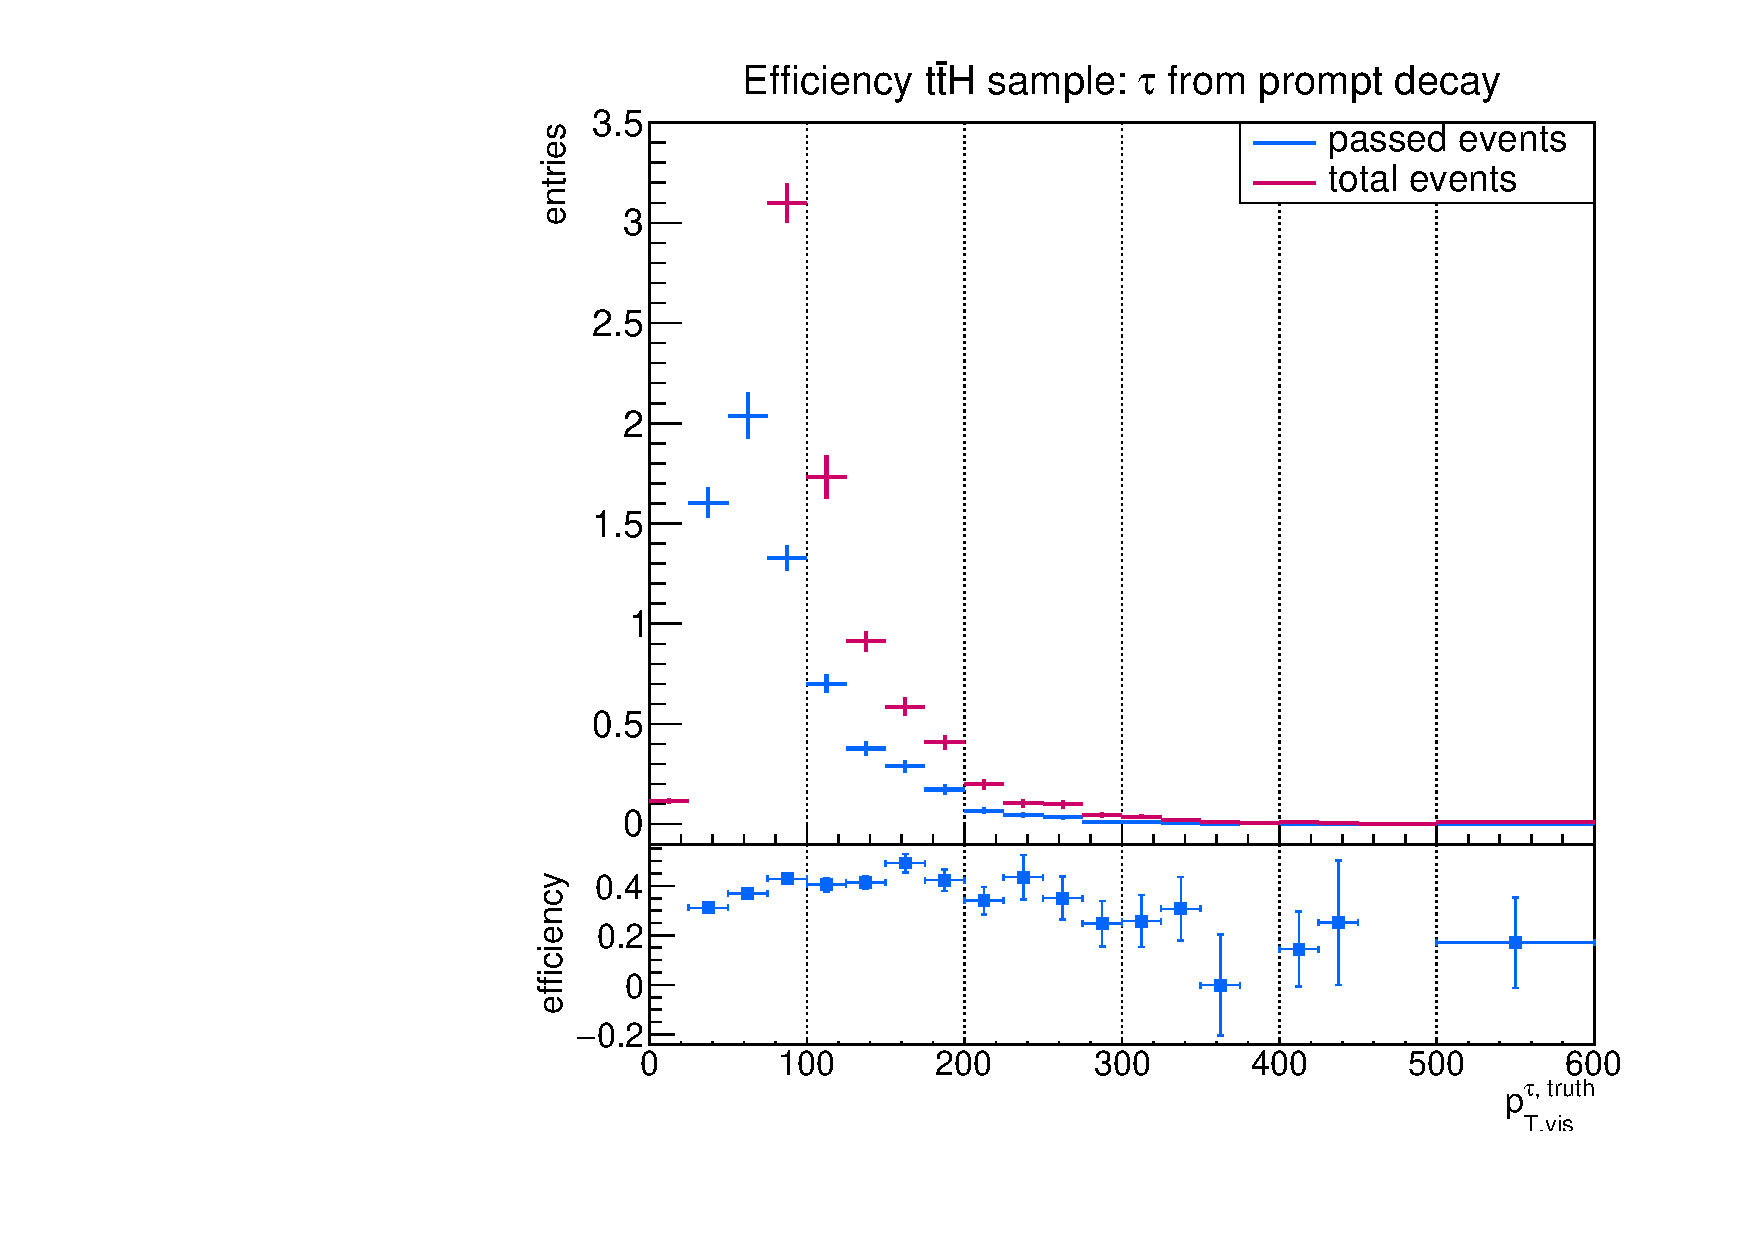
\includegraphics[width=\textwidth]{figures/plots/ttH/Divided_prompt.pdf}
                \subcaption{Efficiency of taus originating from bosons of the weak interaction ($W^\pm$, $Z^0$) of $\SI{36.76\pm 0.51}{\percent}$ for the Higgs events.}
                \label{Dividedprompt:bg:all}
                \end{subfigure}
                %
                \begin{subfigure}[t]{0.49\textwidth}
                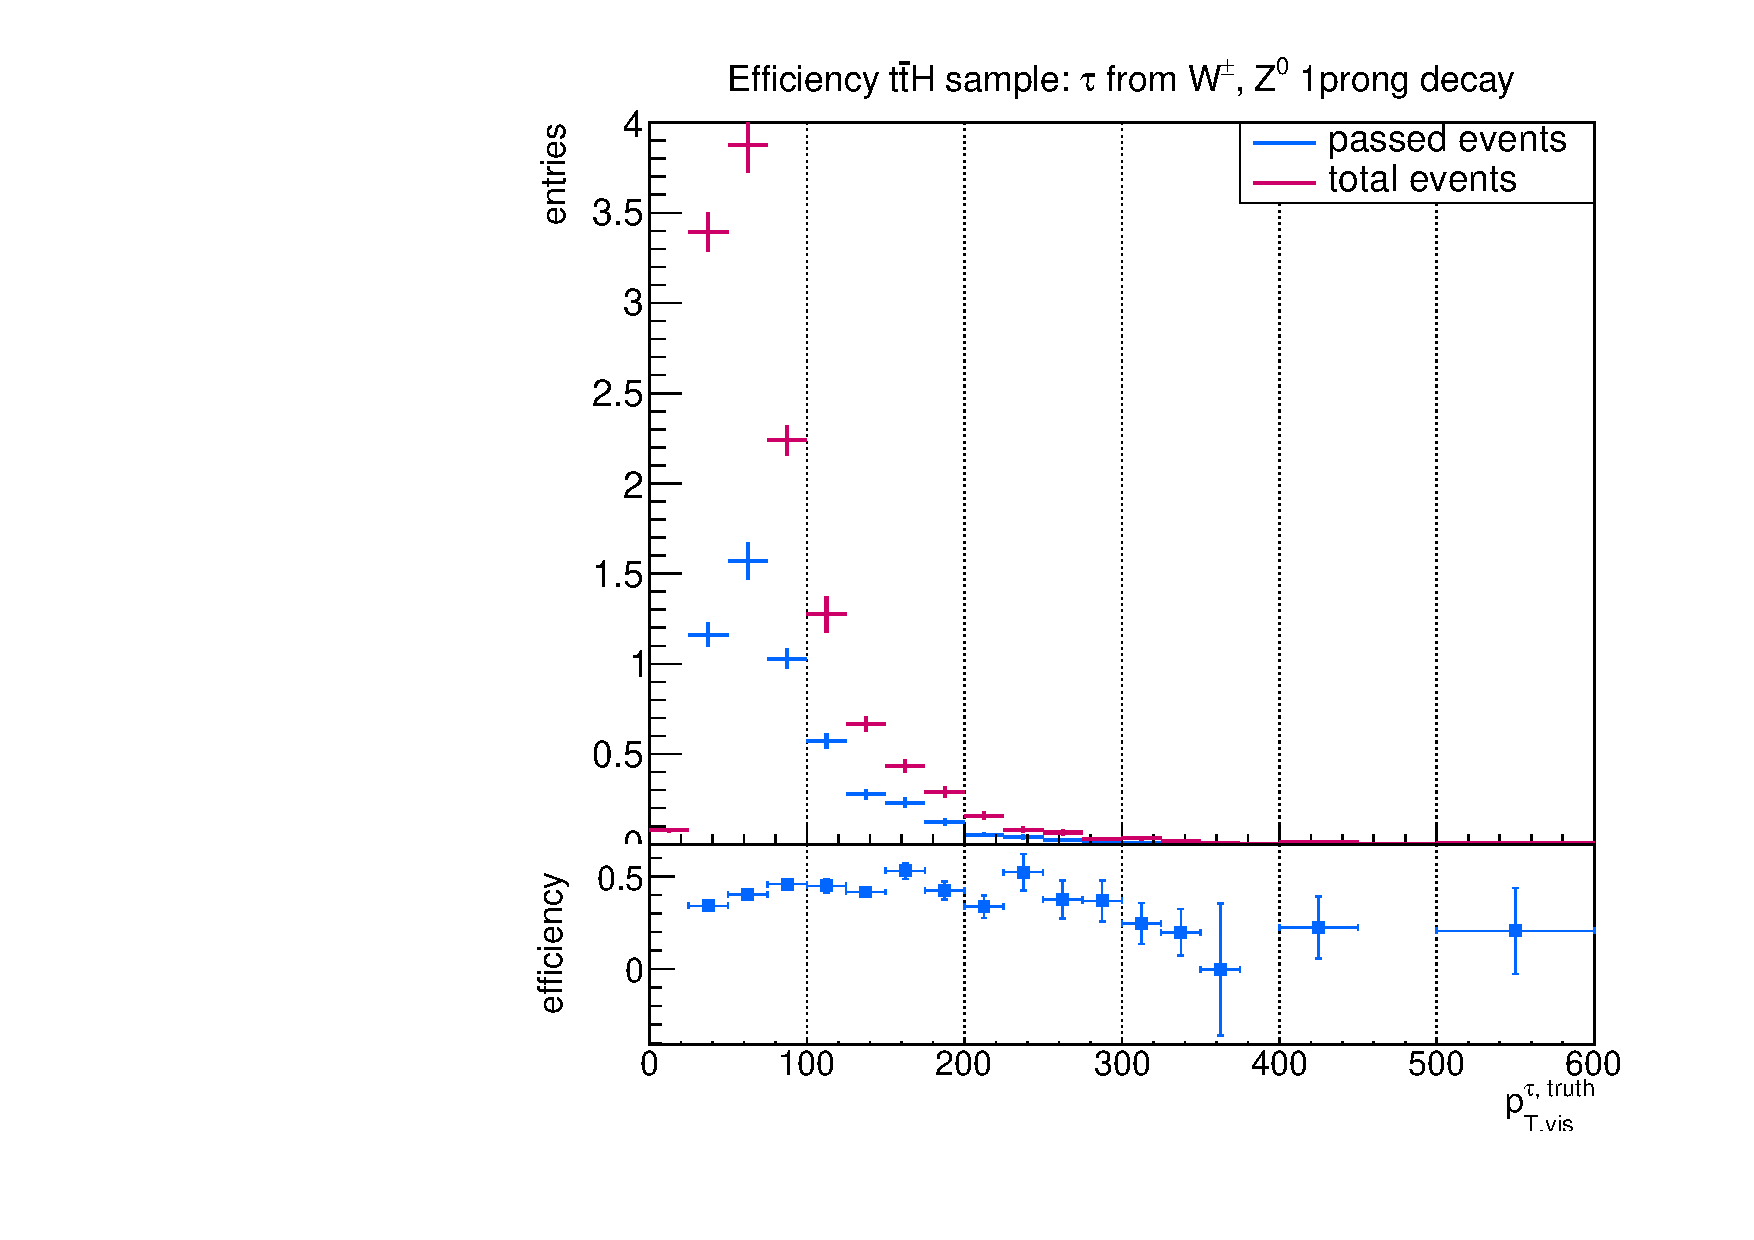
\includegraphics[width=\textwidth]{figures/plots/ttH/Divided_prompt1prong.pdf}
                \subcaption{Efficiency of taus originating from bosons of the weak interaction ($W^\pm$, $Z^0$) and decaying in the 1-prong mode. The efficiency is $\SI{40.16\pm 0.62}{\percent}$ for the Higgs events.}
                \label{Dividedprompt:bg:1prong}
                \end{subfigure}
                %
                \begin{subfigure}[t]{0.49\textwidth}
                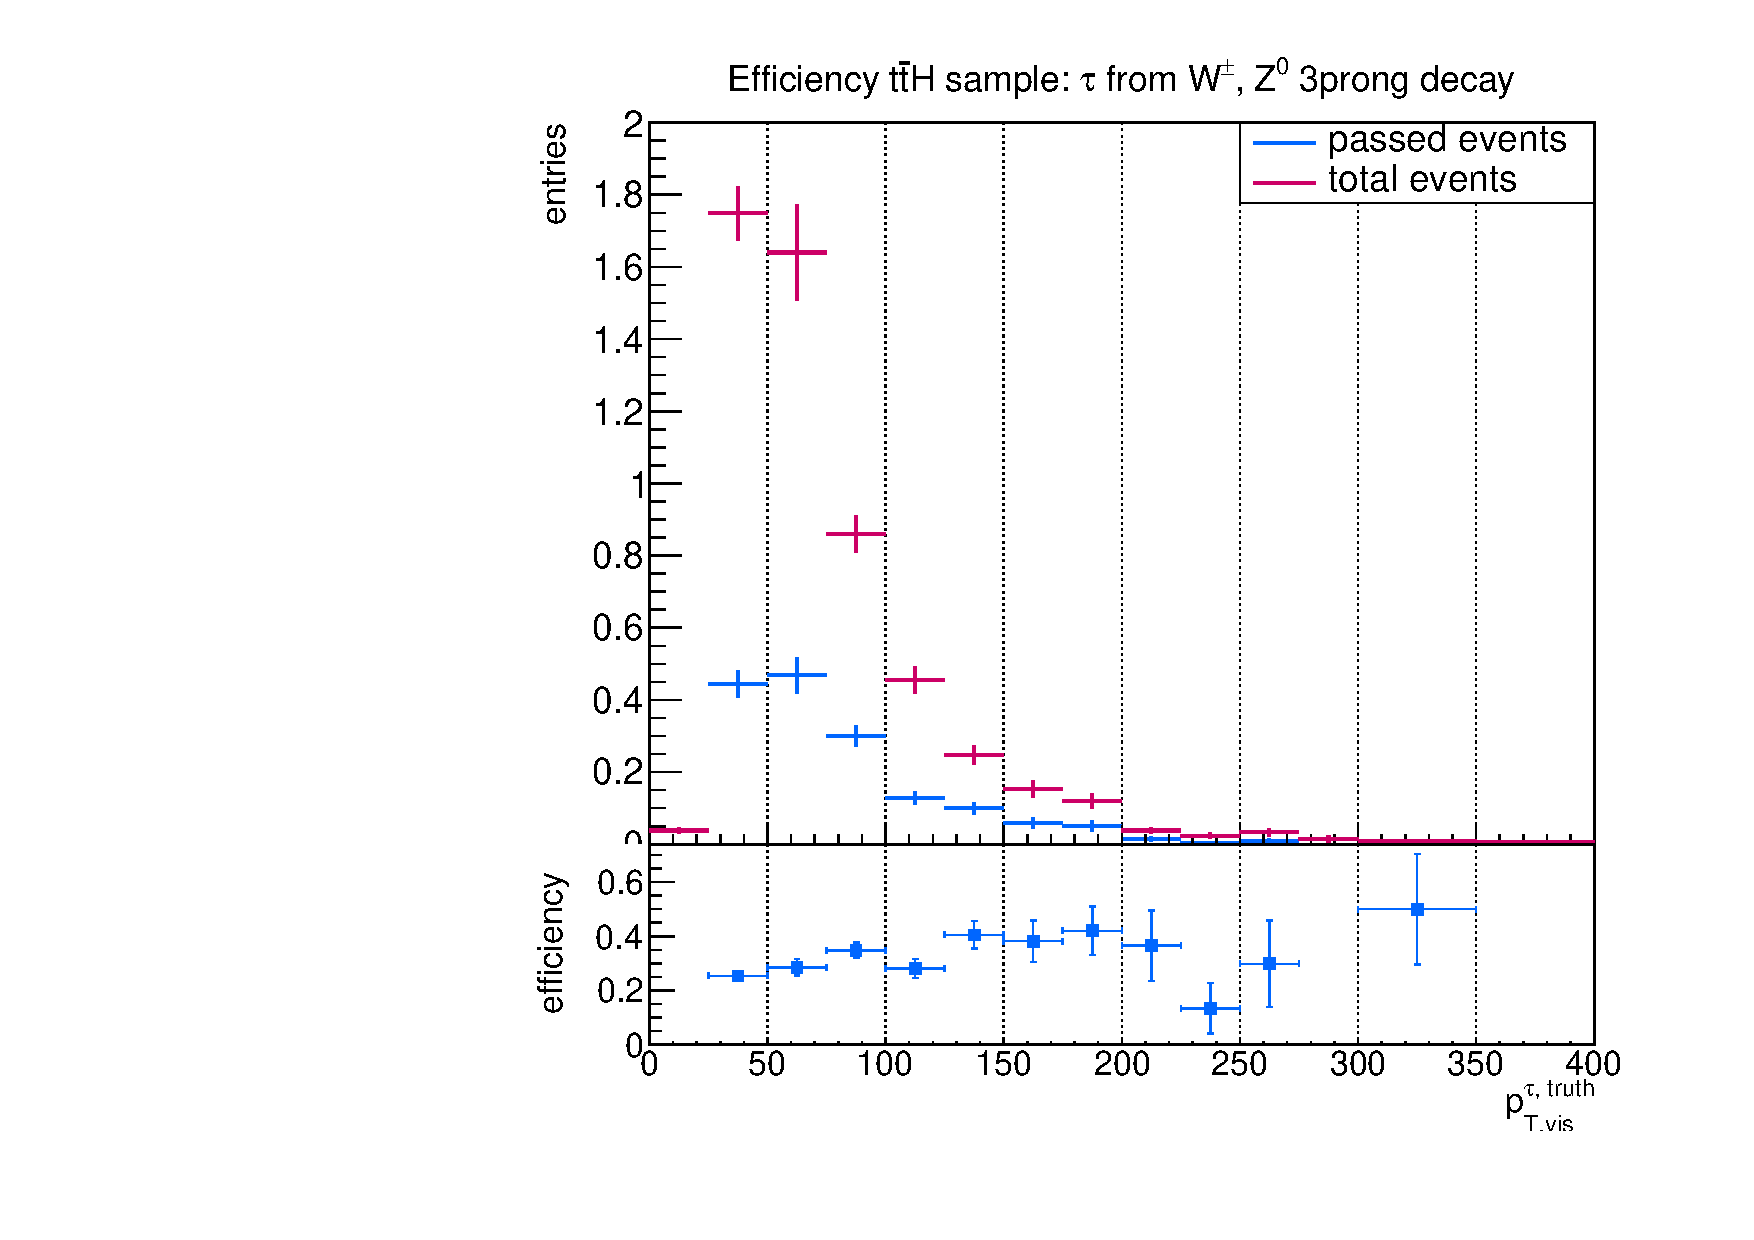
\includegraphics[width=\textwidth]{figures/plots/ttH/Divided_prompt3prong.pdf}
                \subcaption{Efficiency of taus originating from bosons of the weak interaction ($W^\pm$, $Z^0$) and decaying in the 3-prong mode. The efficiency is $\SI{29.01\pm 0.88}{\percent}$ for the Higgs events.}
                \label{Dividedprompt:bg:3prong}
                \end{subfigure}
   %             
\caption[Efficiency of taus originating from bosons of the weak interaction ($W^\pm$, $Z^0$) for the Higgs background events.]{Efficiency of taus originating from bosons of the weak interaction ($W^\pm$, $Z^0$) for the Higgs background events. The efficiency is defined as the number of taus passing the basic selection and matched to a hadronic truth tau as well as the origin is from a $W^\pm$ or $Z^0$ boson over the total number of taus passing the basic selection and originating from a $W^\pm$ or $Z^0$ boson.}
\label{Dividedprompt:bg:ttH}
\end{figure}
%
%
\begin{figure}
  \centering
                \begin{subfigure}[t]{0.49\textwidth}
                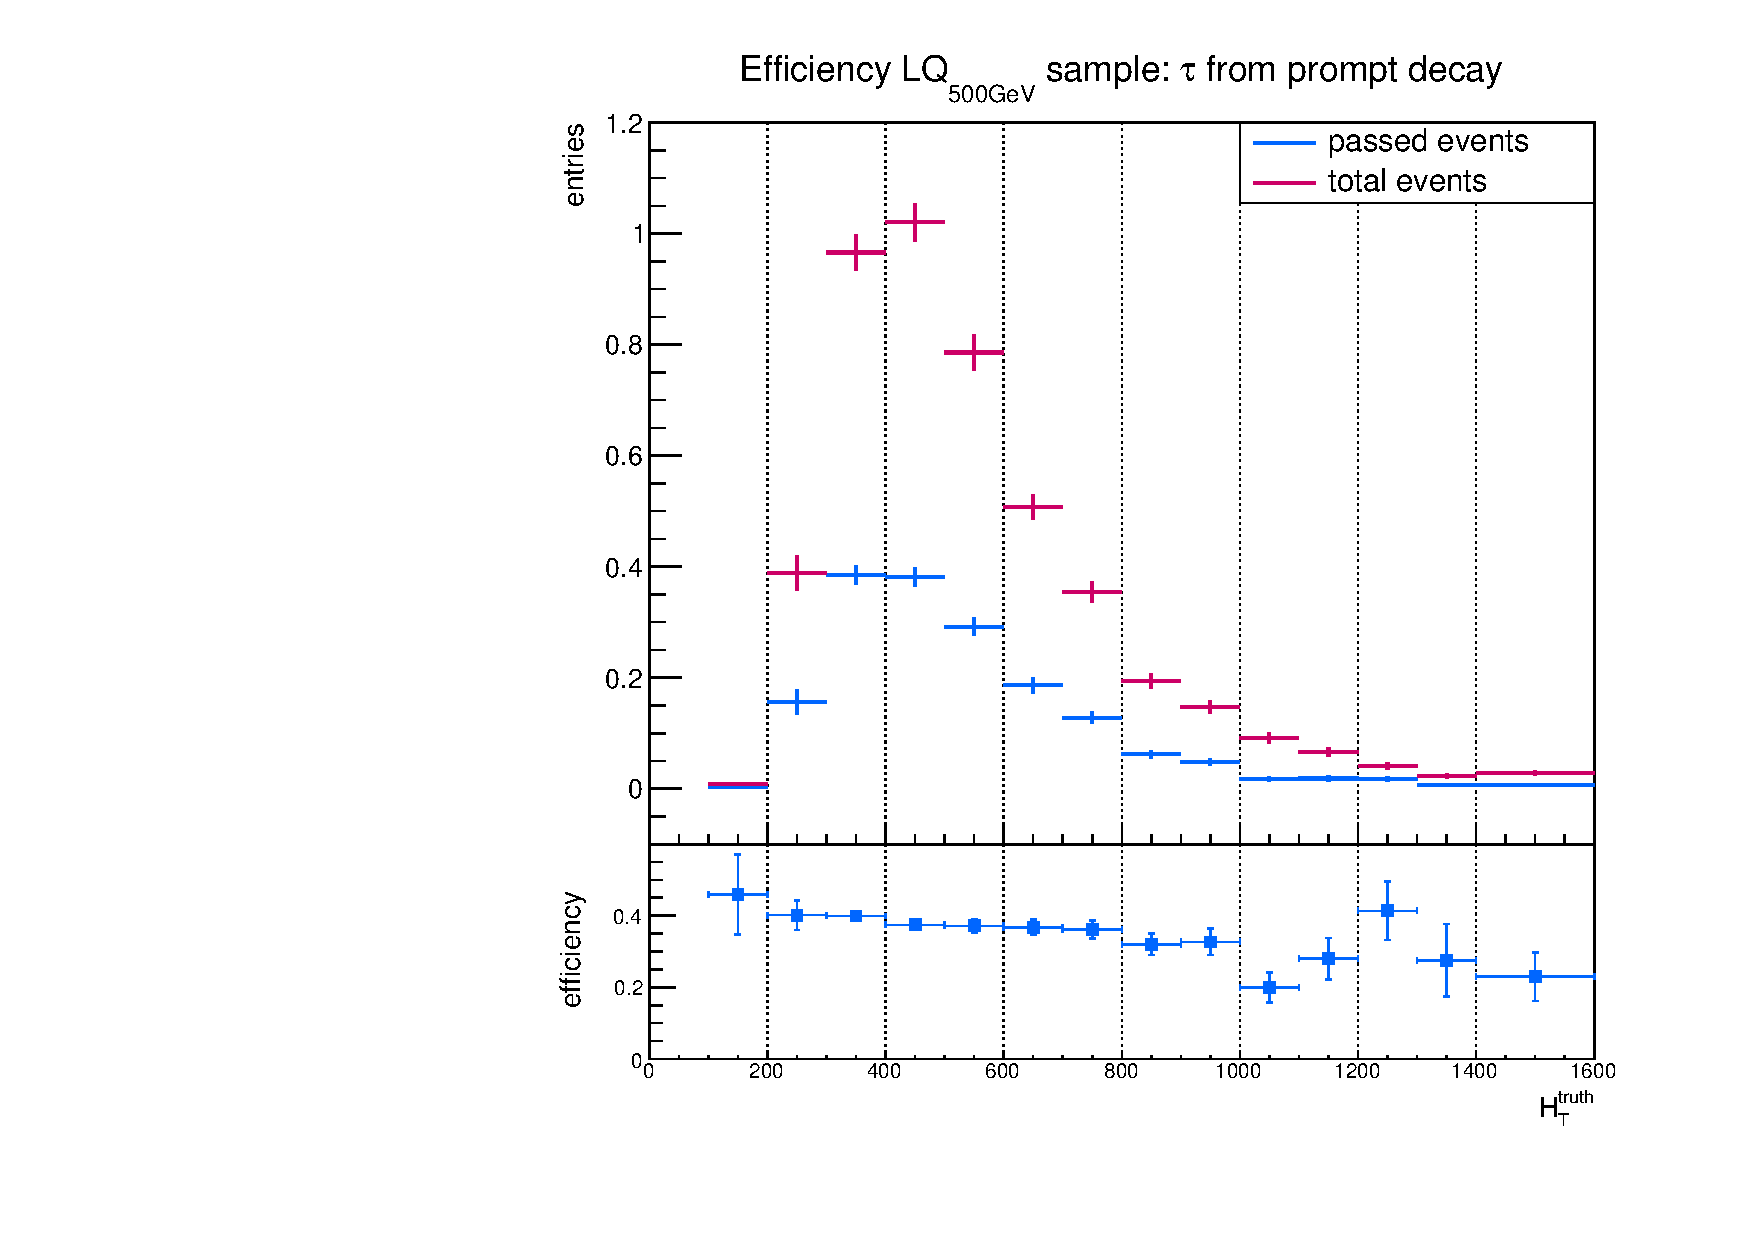
\includegraphics[width=\textwidth]{figures/plots/ttH/Divided_promptHT.pdf}
                \subcaption{Efficiency of taus originating from $W^\pm$, and $Z^0$ bosons of depending on $H_{T}$ for the Higgs events.}
                \label{Divided:prompt:HT}
                \end{subfigure}
                %
                \begin{subfigure}[t]{0.49\textwidth}
                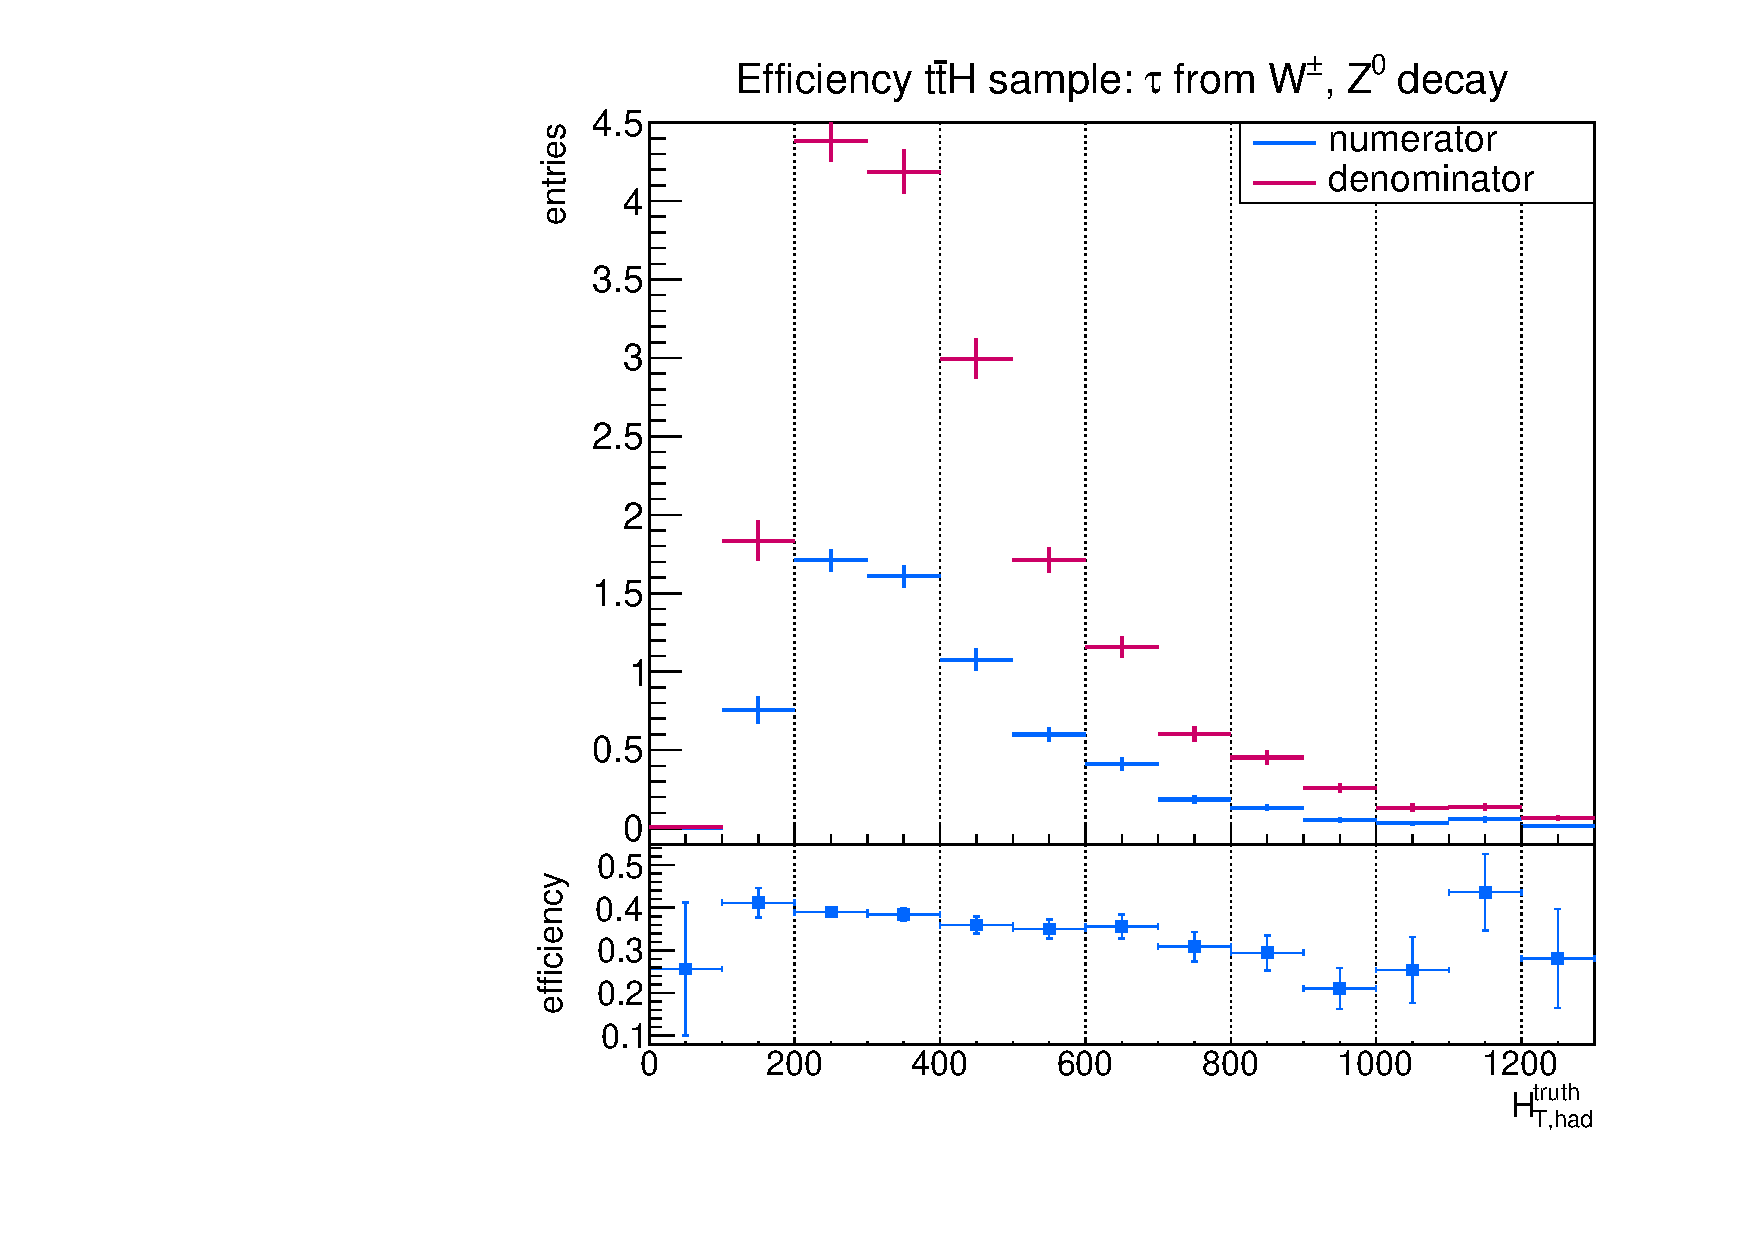
\includegraphics[width=\textwidth]{figures/plots/ttH/Divided_promptHThad.pdf}
                \subcaption{Efficiency of taus originating from $W^\pm$, and $Z^0$ bosons of depending on $H_{T,\text{had}}$ for the Higgs events.}
                \label{Divided:prompt:HThad}
                \end{subfigure}
\caption[Efficiency of taus originating from $W^\pm$, and $Z^0$ bosons for the Higgs background events.]{Efficiency of taus originating from $W^\pm$, and $Z^0$ bosons depending on $H_{T}$ (a) and $H_{T,\text{had}}$ (b)for the Higgs background events.}
\label{Divided:prompt:HTgedöns}
\end{figure}
%
%
\begin{figure}
  \centering
                \begin{subfigure}[t]{0.49\textwidth}
                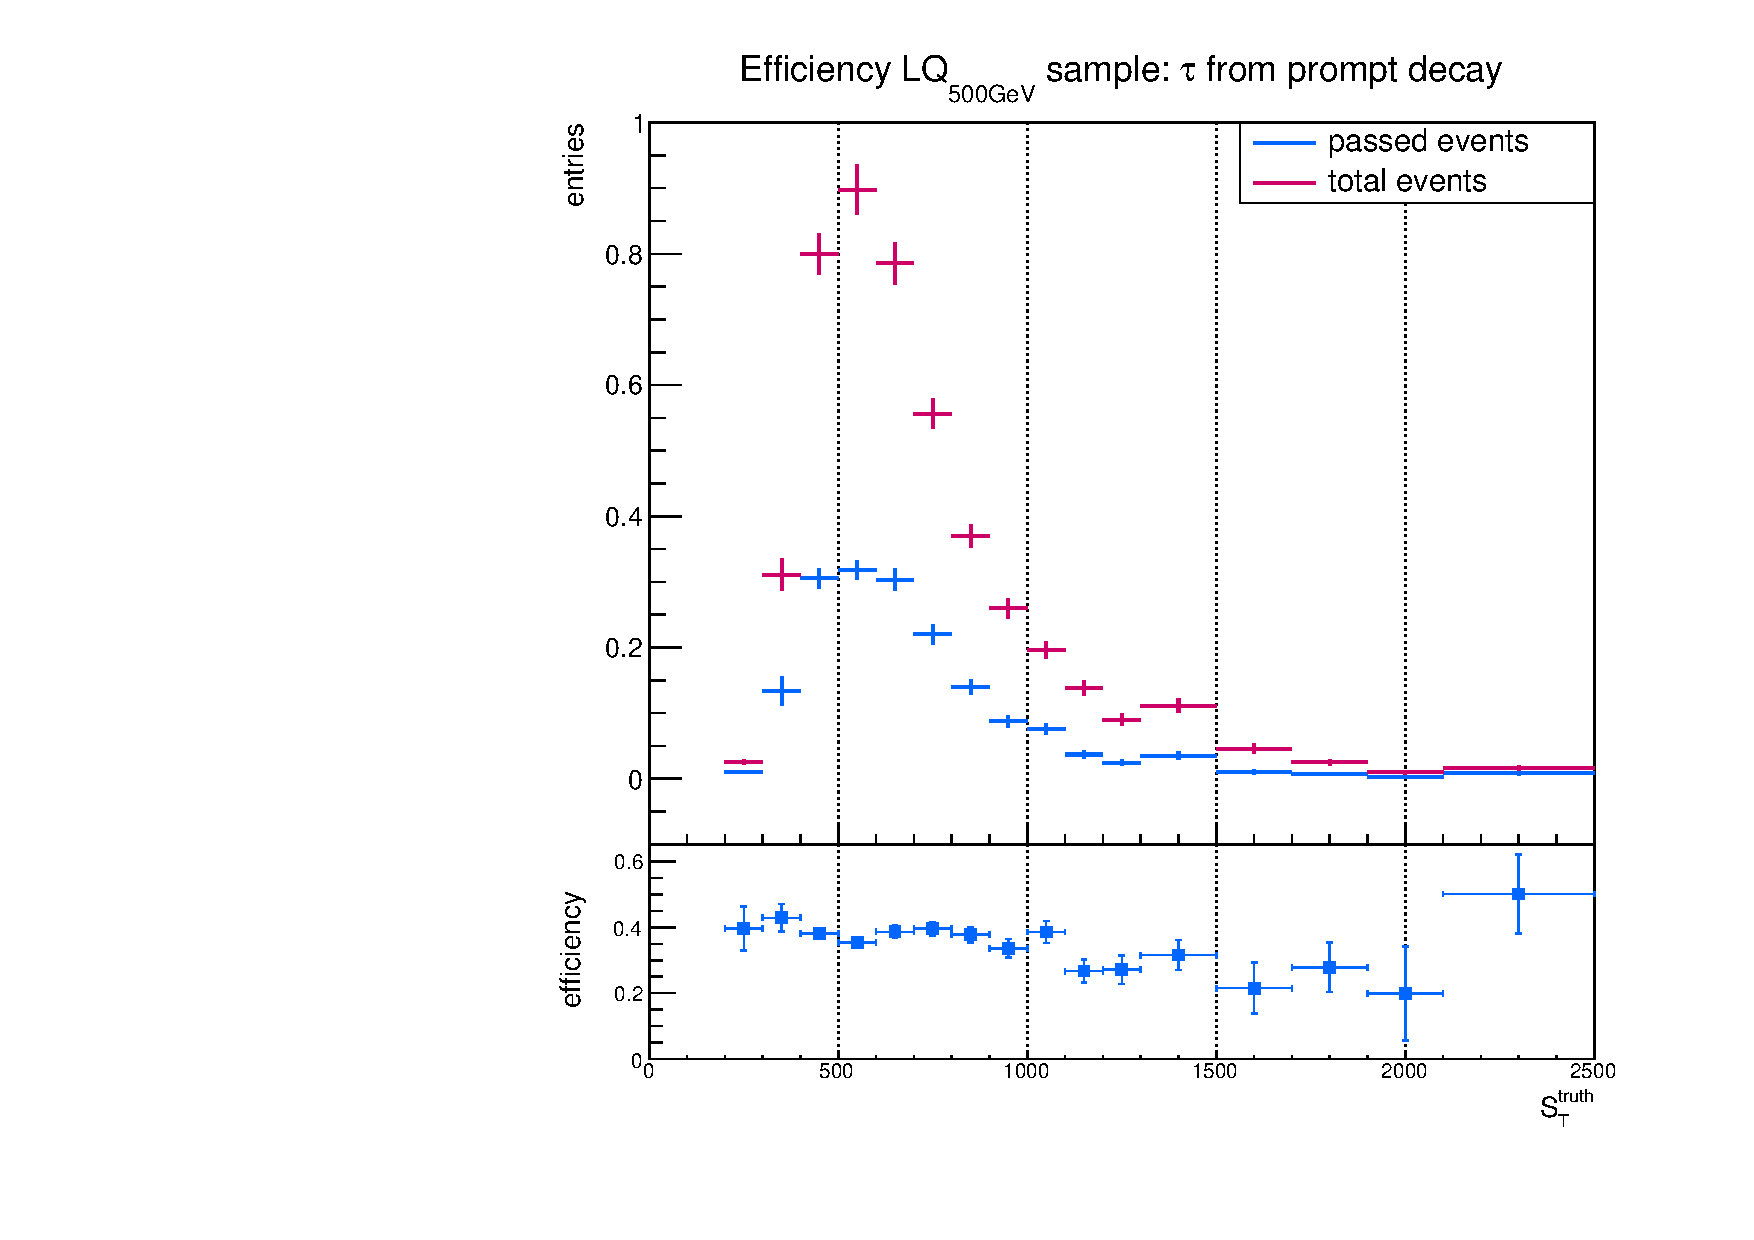
\includegraphics[width=\textwidth]{figures/plots/ttH/Divided_promptST.pdf}
                \subcaption{Efficiency of taus originating from $W^\pm$, and $Z^0$ bosons of depending on $S_{T}$ for the Higgs events.}
                \label{Divided:prompt:ST}
                \end{subfigure}
                %
                \begin{subfigure}[t]{0.49\textwidth}
                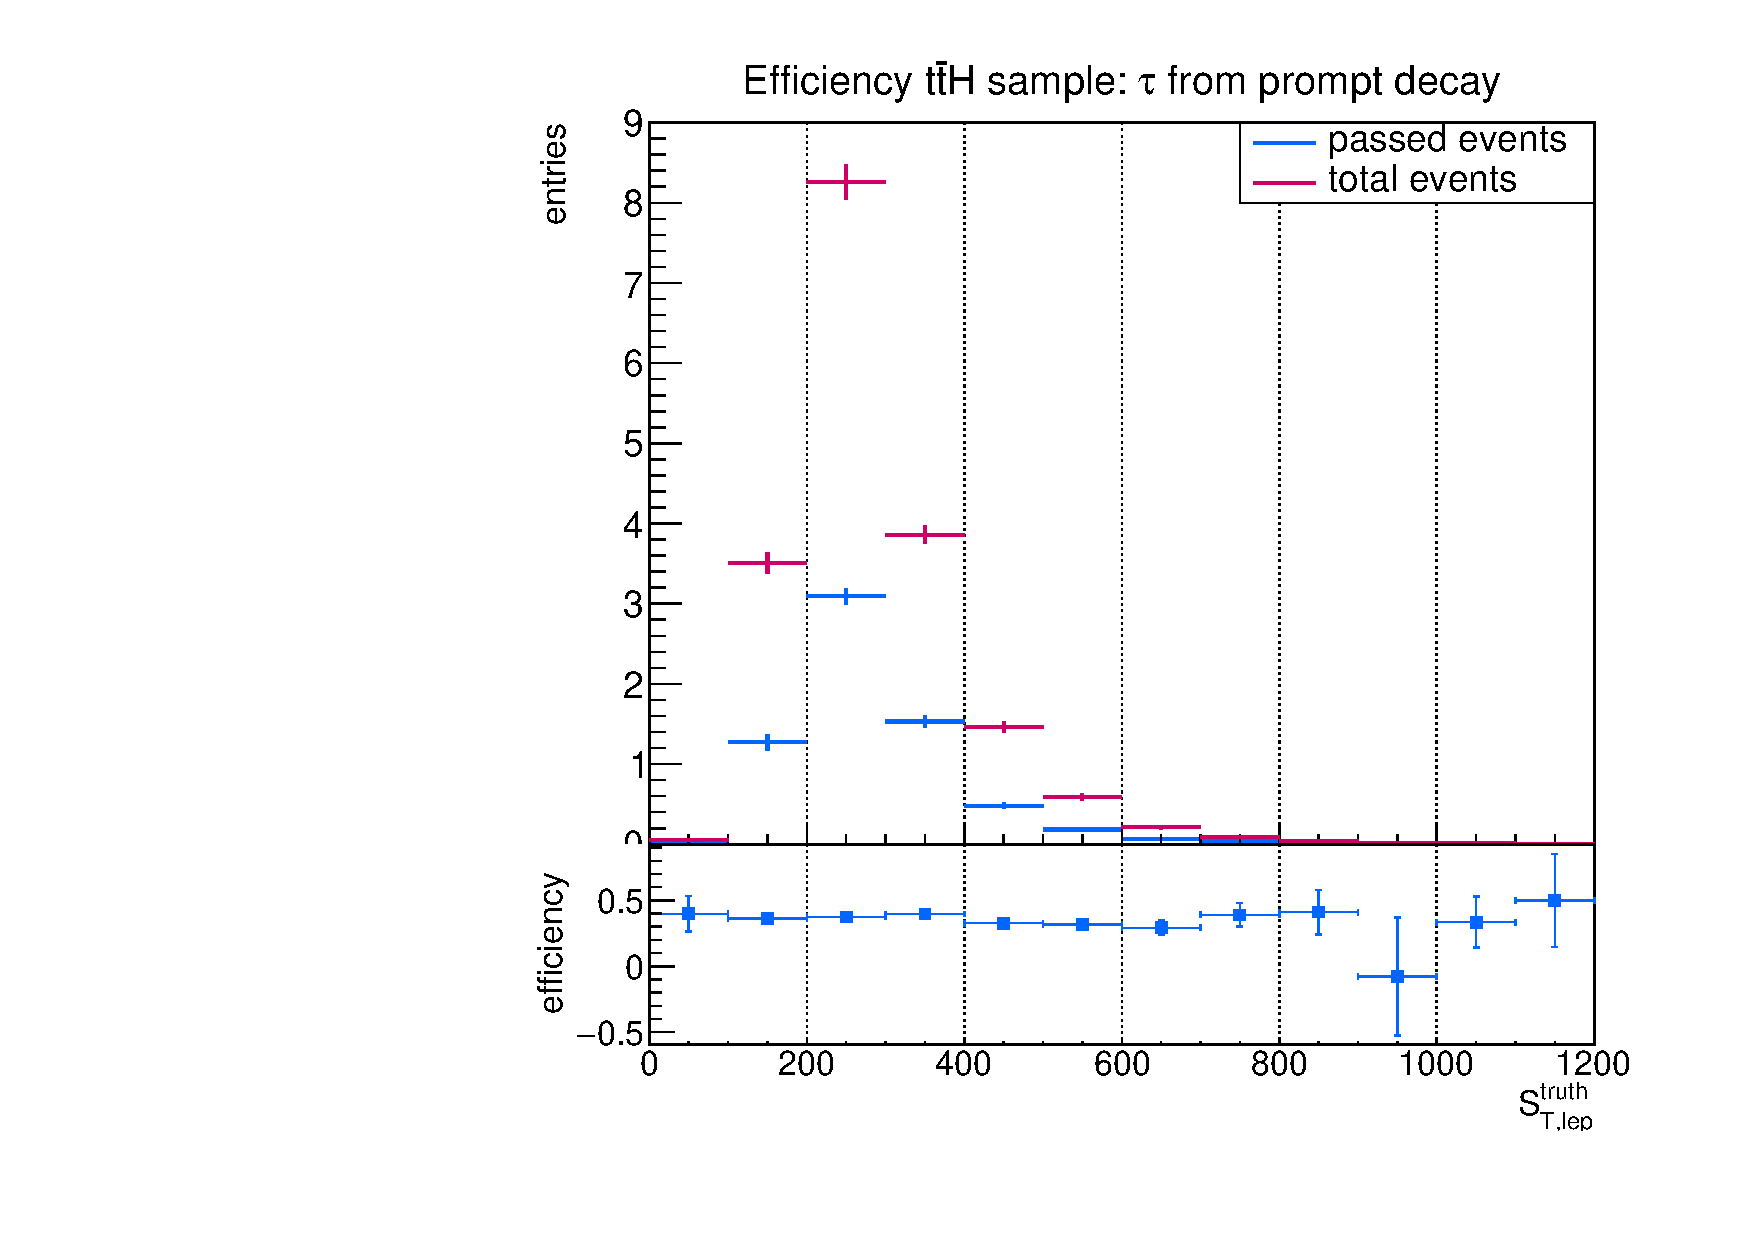
\includegraphics[width=\textwidth]{figures/plots/ttH/Divided_promptSTlep.pdf}
                \subcaption{Efficiency of taus originating from $W^\pm$, and $Z^0$ bosons of depending on $S_{T,\text{lep}}$ for the Higgs events.}
                \label{Divided:prompt:STlep}
\end{subfigure}
\caption[Efficiency of taus originating from $W^\pm$, and $Z^0$ bosons for the Higgs background events.]{Efficiency of taus originating from $W^\pm$, and $Z^0$ bosons depending on $S_{T}$ (a) and $S_{T,\text{lep}}$ (b) for the Higgs background events.}
\label{Divided:prompt:STgedöns}
\end{figure}
%
%
\begin{figure}
                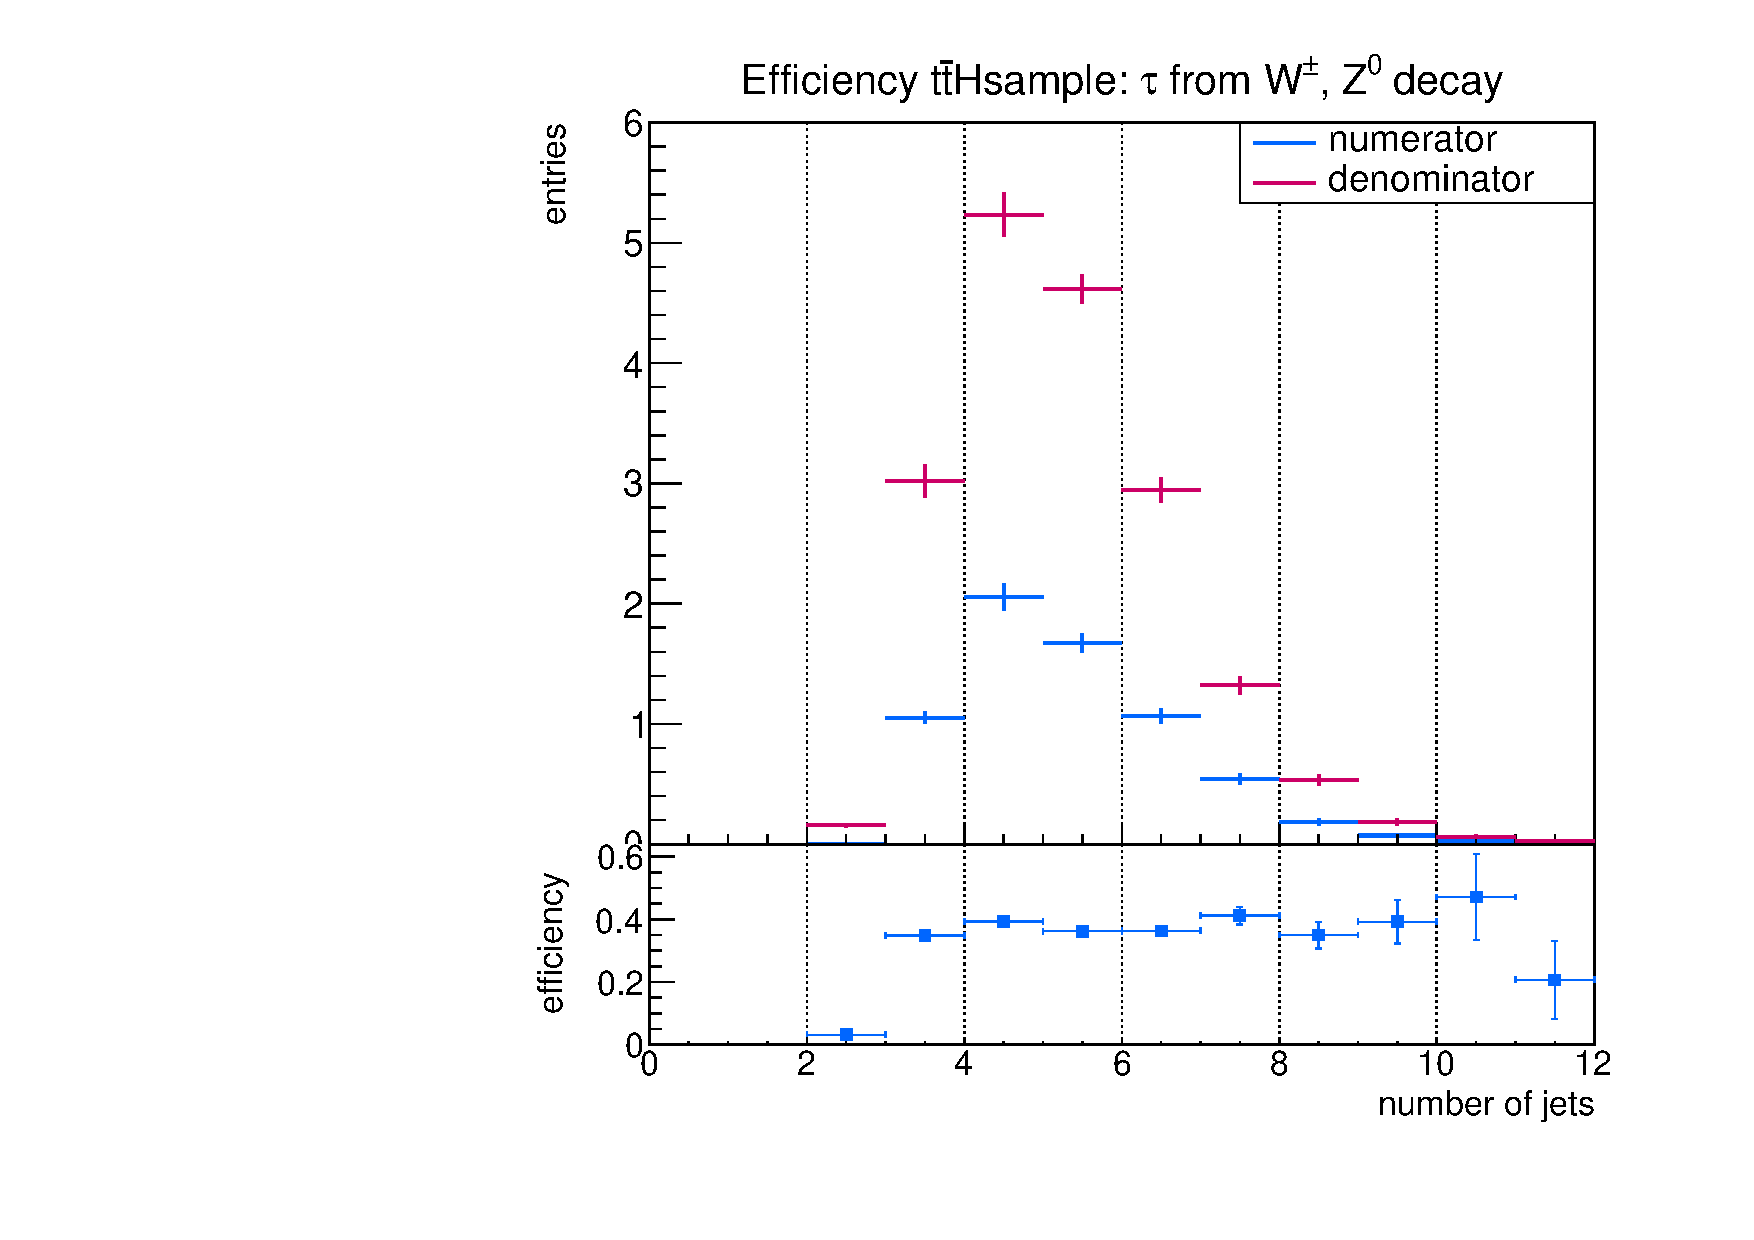
\includegraphics[width=\textwidth]{figures/plots/ttH/Divided_promptnjets.pdf}
                \caption{Efficiency of taus originating from $W^\pm$ and $Z^0$ bosons depending on the number of jets for the Higgs events.}
         \label{Divided:prompt:njets}
\end{figure}
%
%
%
\begin{figure}
  \centering
                \begin{subfigure}[t]{0.49\textwidth}
                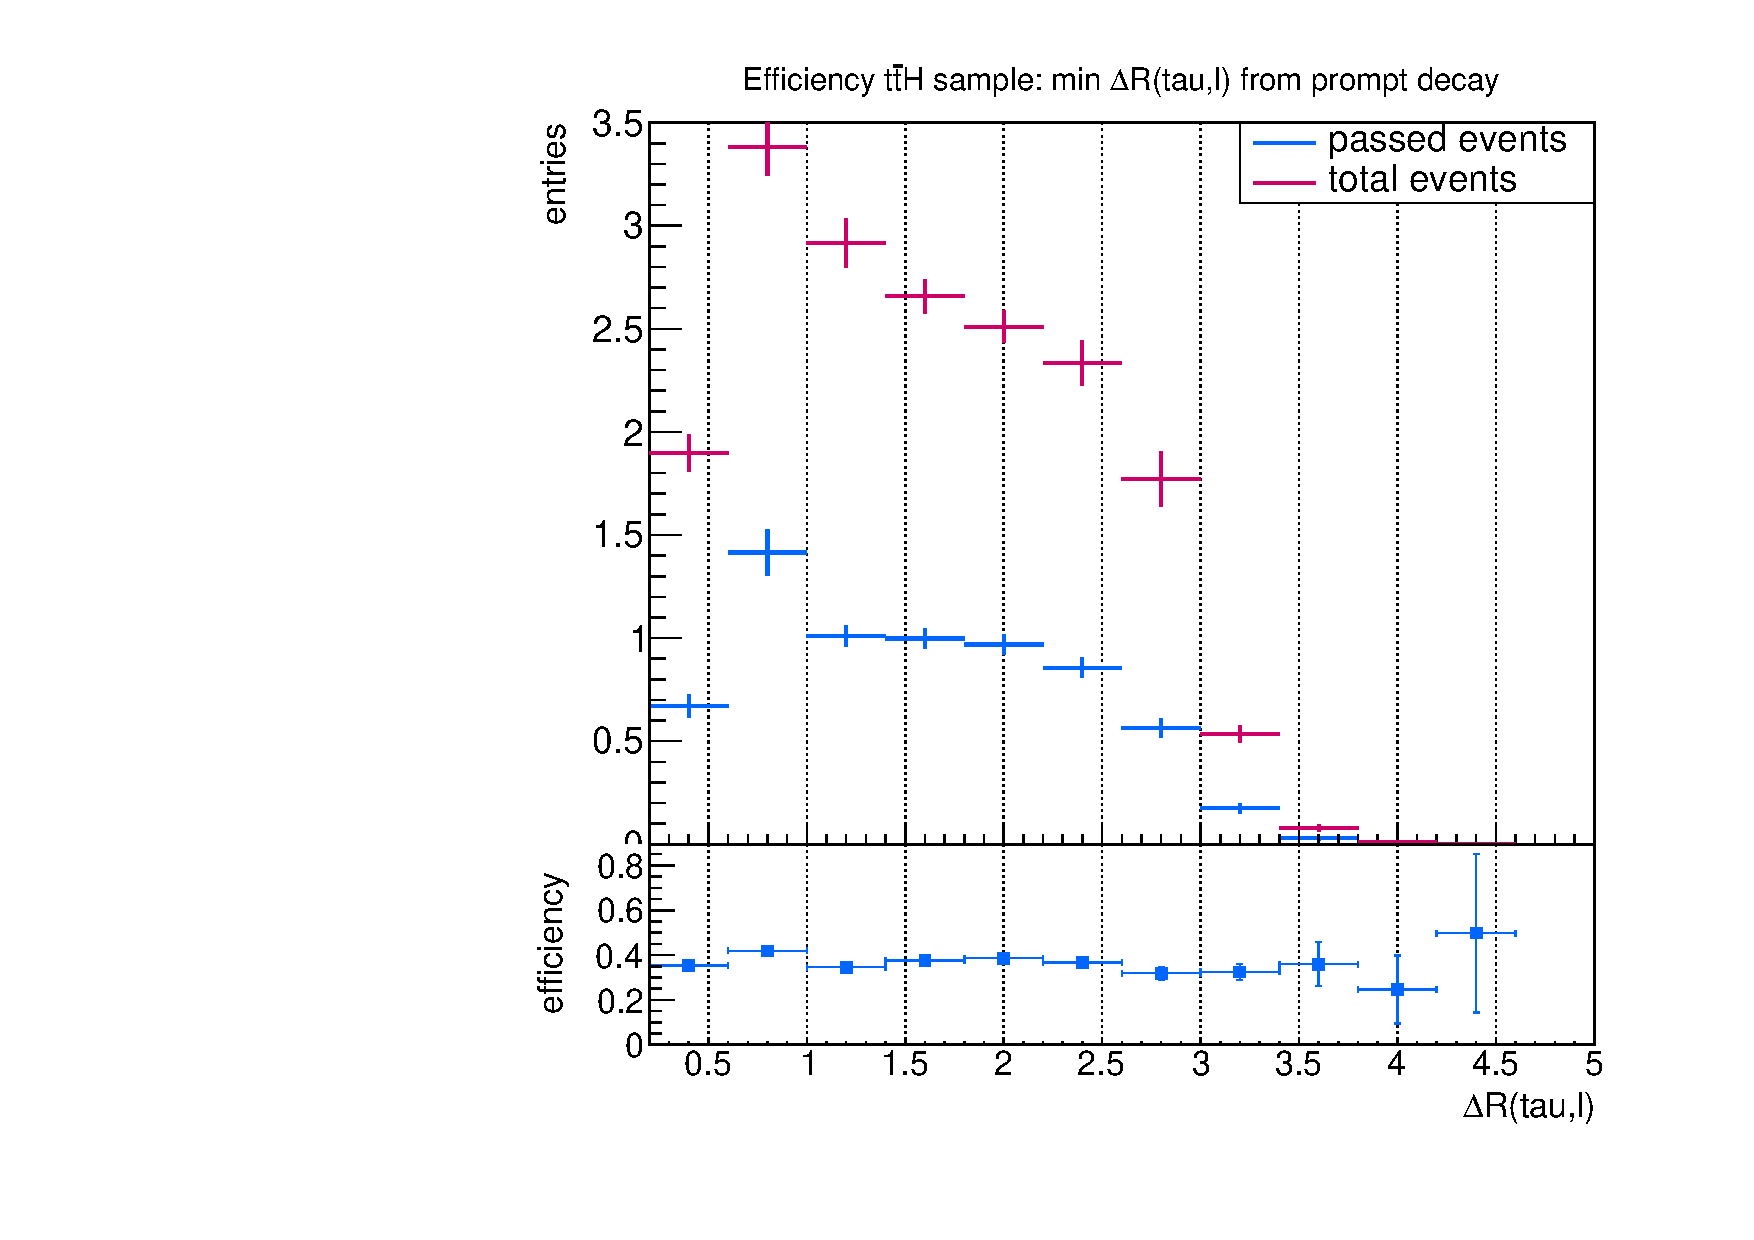
\includegraphics[width=\textwidth]{figures/plots/ttH/Divided_pr_mindR_taulepton.pdf}
                \subcaption{Minimum separation between taus originating from $W^\pm$, $Z^0$ events and leptons.}
                \label{dR:prompt:taulepton:min}
                \end{subfigure}
                %
                \begin{subfigure}[t]{0.49\textwidth}
                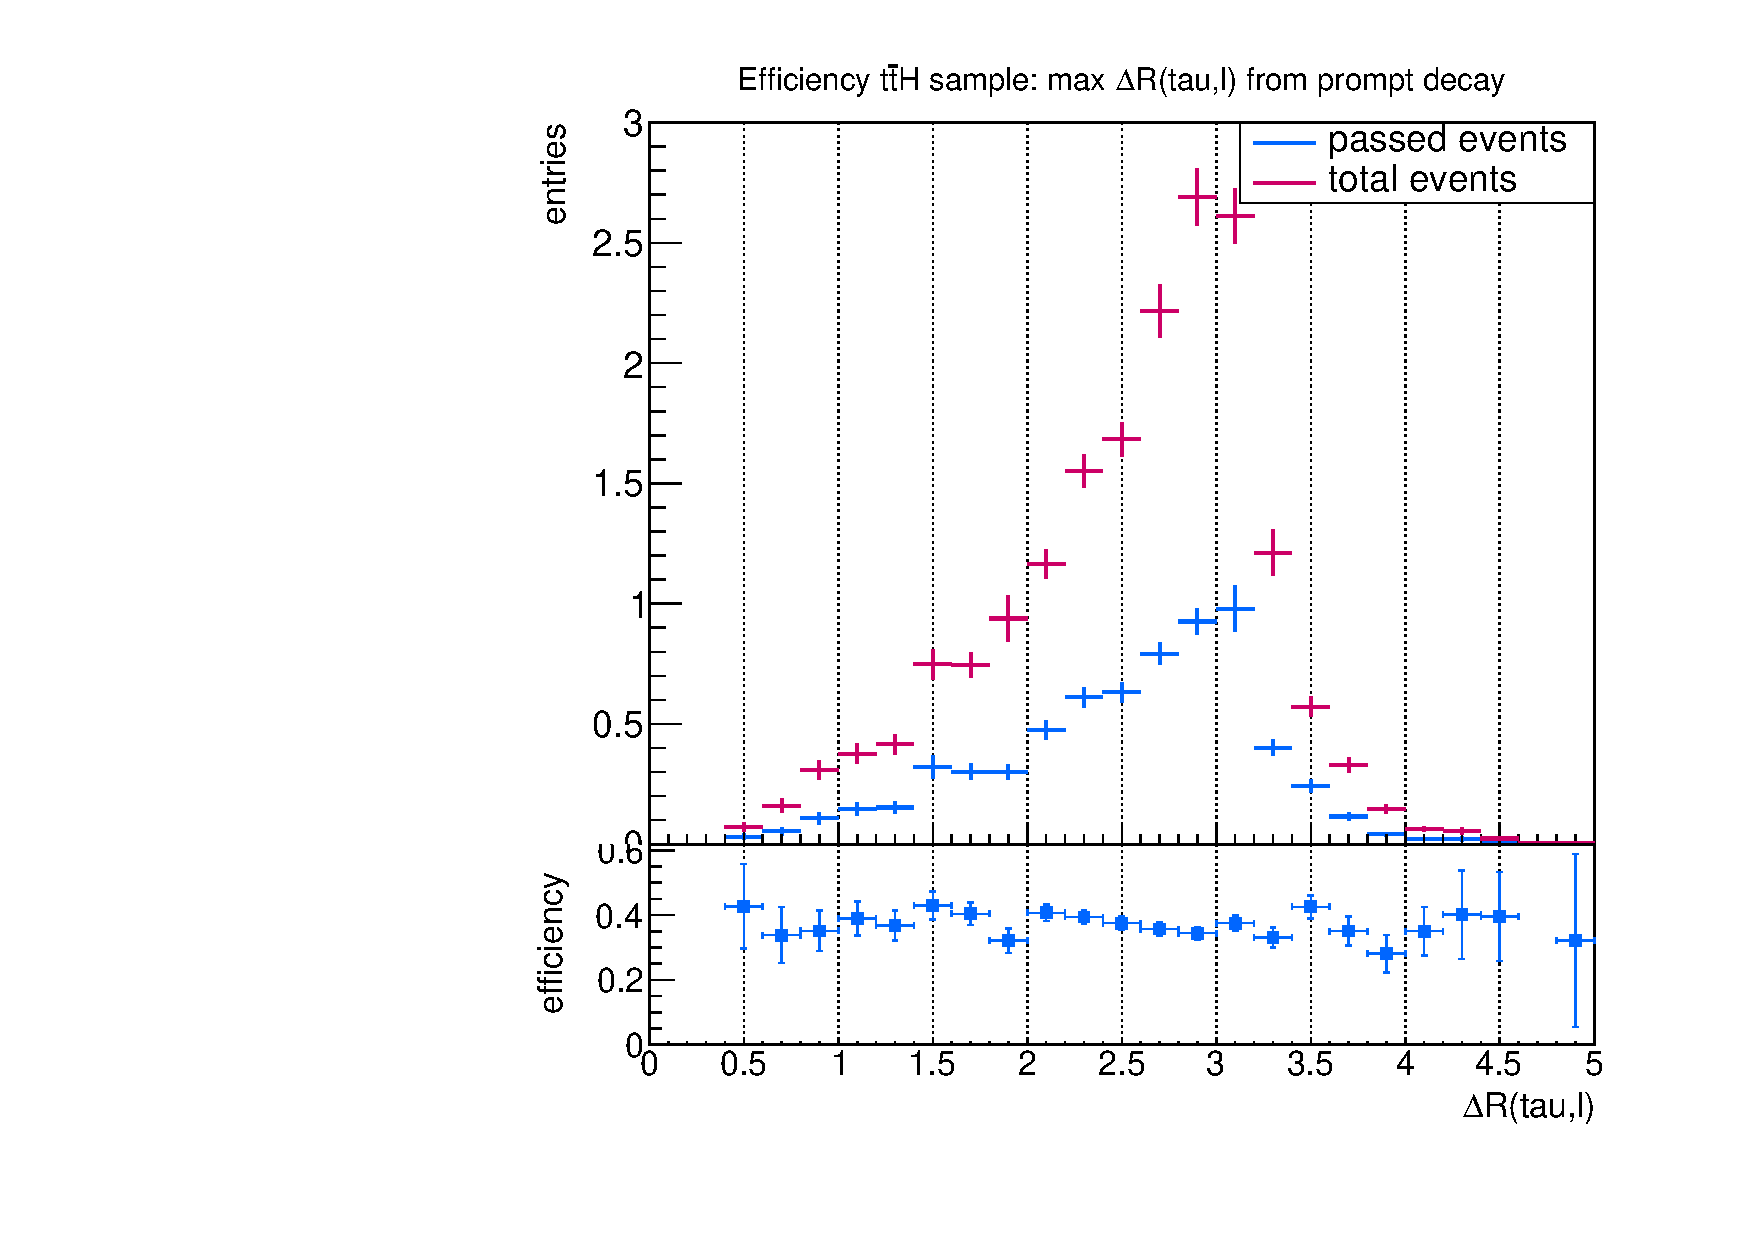
\includegraphics[width=\textwidth]{figures/plots/ttH/Divided_maxdR_pr_taulepton.pdf}
                \subcaption{Maximum separation between taus originating from $W^\pm$, $Z^0$ events and leptons.}
                \label{dR:prompt:taulepton:max}
                \end{subfigure}
\caption[Efficiency of taus originating from $W^\pm$, $Z^0$ for the separation between taus and leptons.]{Efficiency of taus originating from $W^\pm$, $Z^0$ for the minimum and maximum separation between taus and leptons (electrons and muons).}
\label{dR:prompt:taulepton}
\end{figure}
%
%
\begin{figure}
  \centering
                \begin{subfigure}[t]{0.49\textwidth}
                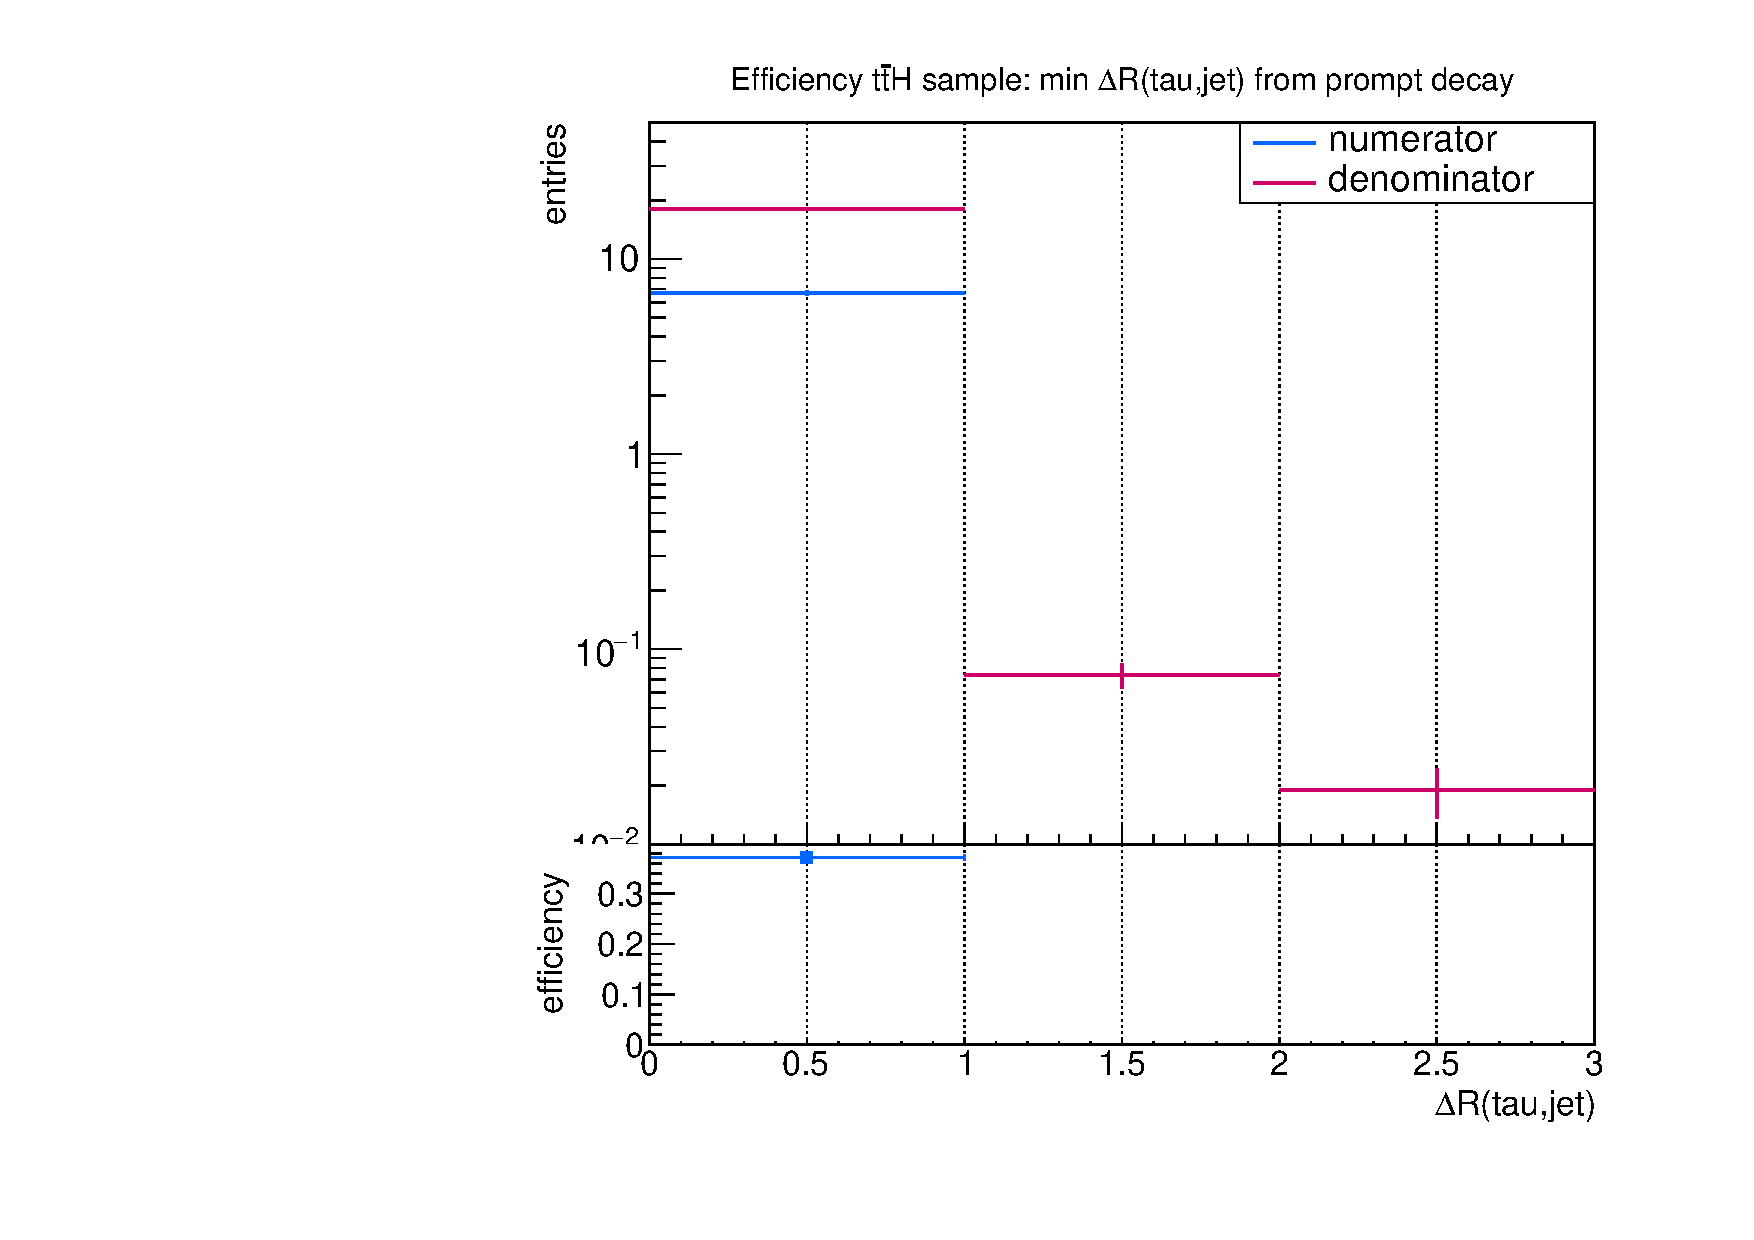
\includegraphics[width=\textwidth]{figures/plots/ttH/Divided_pr_mindR_taujet.pdf}
                \subcaption{Minimum separation between taus originating from $W^\pm$, $Z^0$ events and jets.}
                \label{dR:prompt:taujets:min}
                \end{subfigure}
                %
                \begin{subfigure}[t]{0.49\textwidth}
                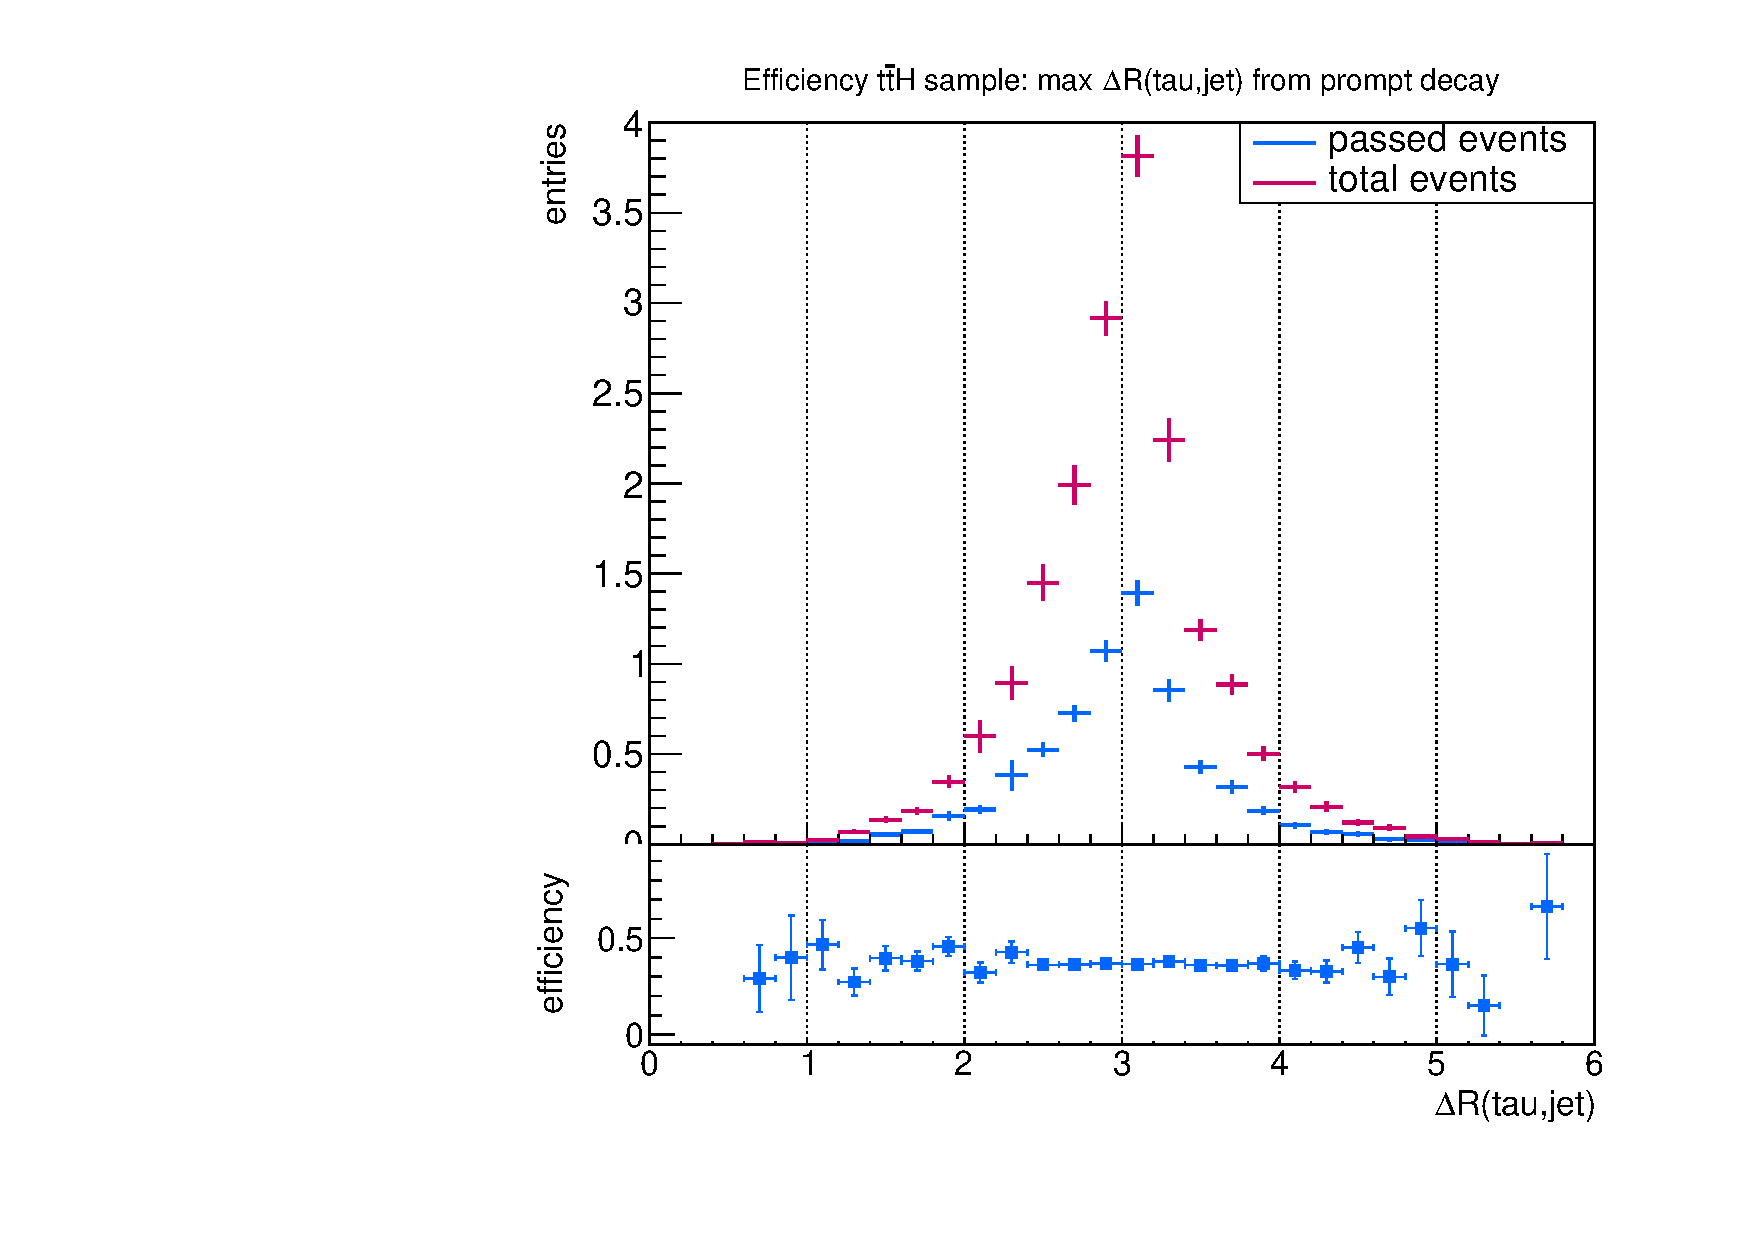
\includegraphics[width=\textwidth]{figures/plots/ttH/Divided_maxdR_pr_taujet.pdf}
                \subcaption{Maximum separation between taus originating from $W^\pm$, $Z^0$ events and jets.}
                \label{dR:prompt:taujets:max}
                \end{subfigure}
\caption[Efficiency of taus originating from $W^\pm$, $Z^0$ for the separation between taus and jets.]{Efficiency of taus originating from $W^\pm$, $Z^0$ for the minimum and maximum separation between taus and jets.}
\label{dR:prompt:taujets}
\end{figure}
%
%
\begin{figure}
  \centering
                \begin{subfigure}[t]{0.49\textwidth}
                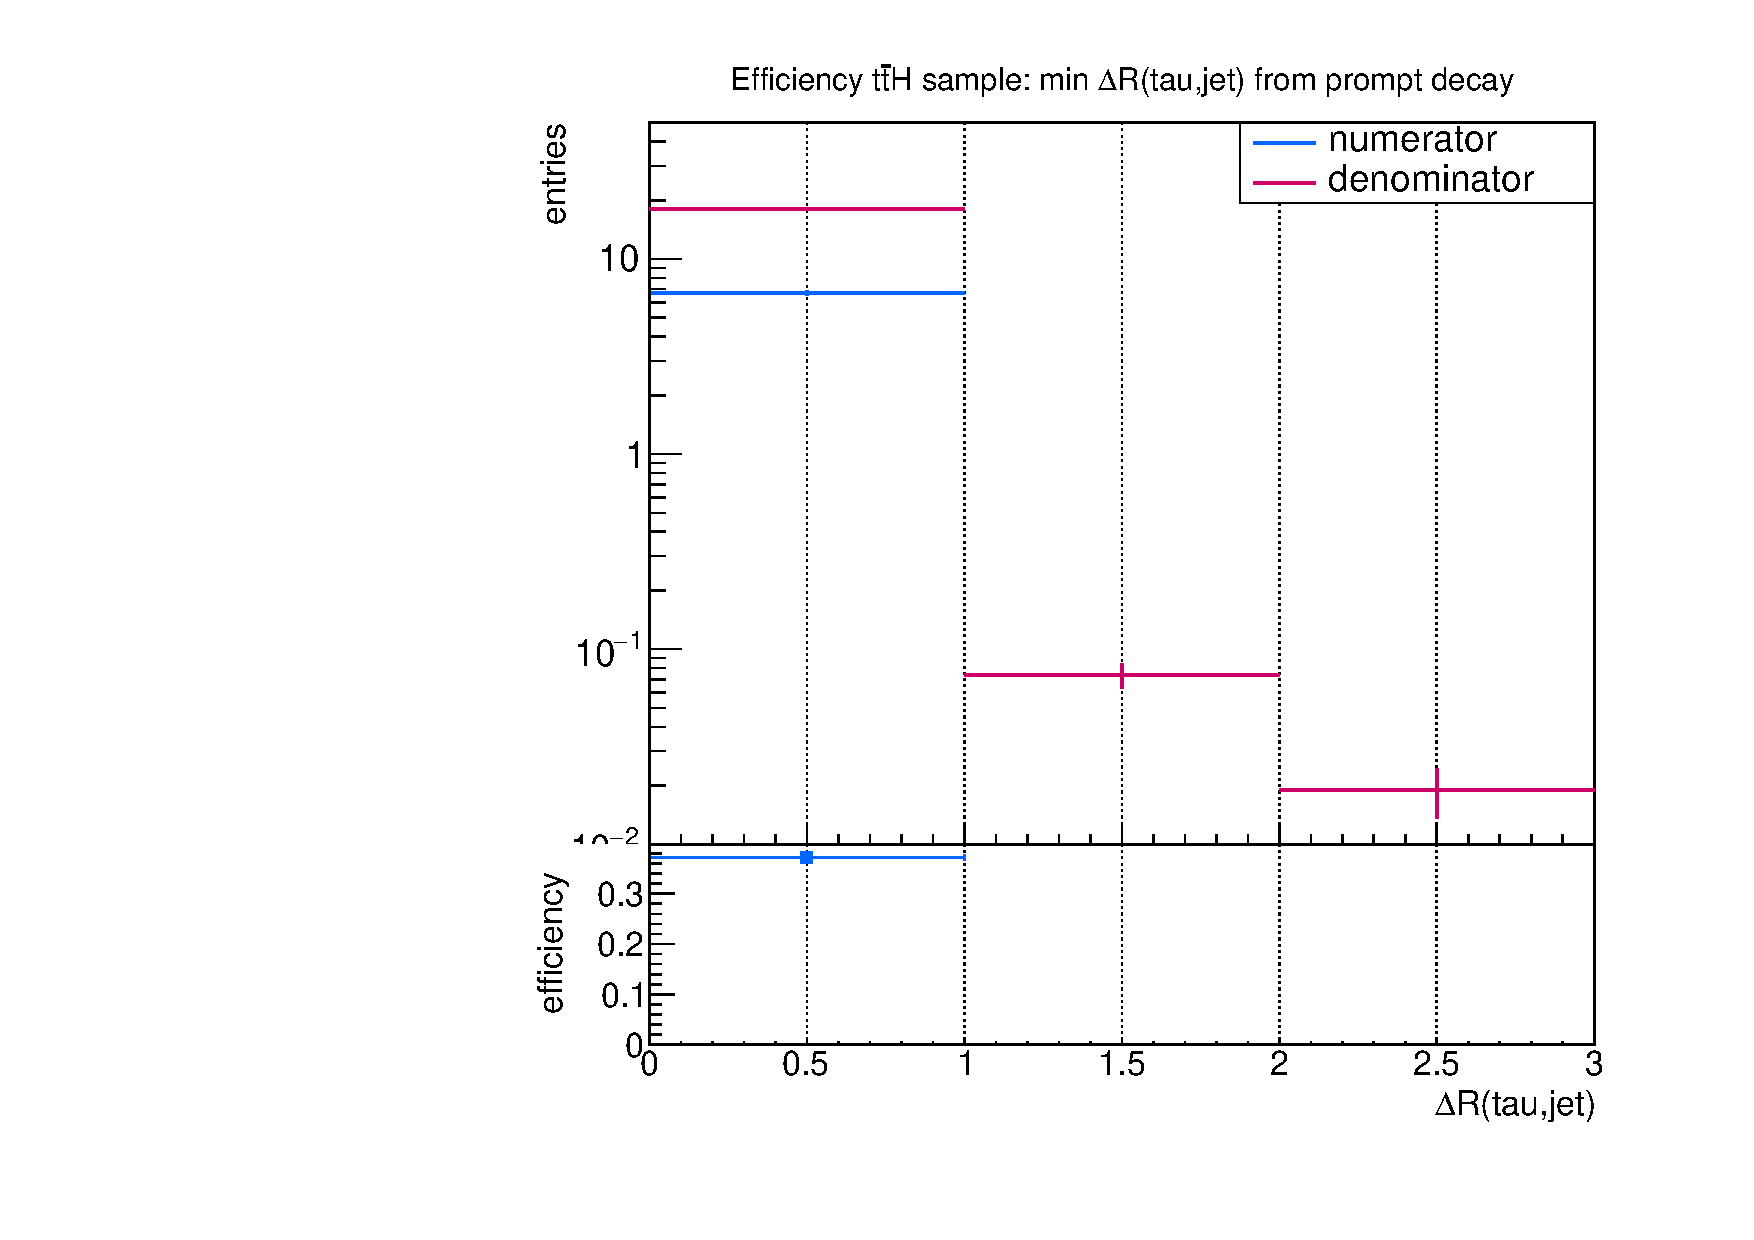
\includegraphics[width=\textwidth]{figures/plots/ttH/Divided_pr_mindR_taujet.pdf}
                \subcaption{Minimum separation between taus originating from $W^\pm$, $Z^0$ events and b-jets.}
                \label{dR:prompt:taubjets:min}
                \end{subfigure}
                %
                \begin{subfigure}[t]{0.49\textwidth}
                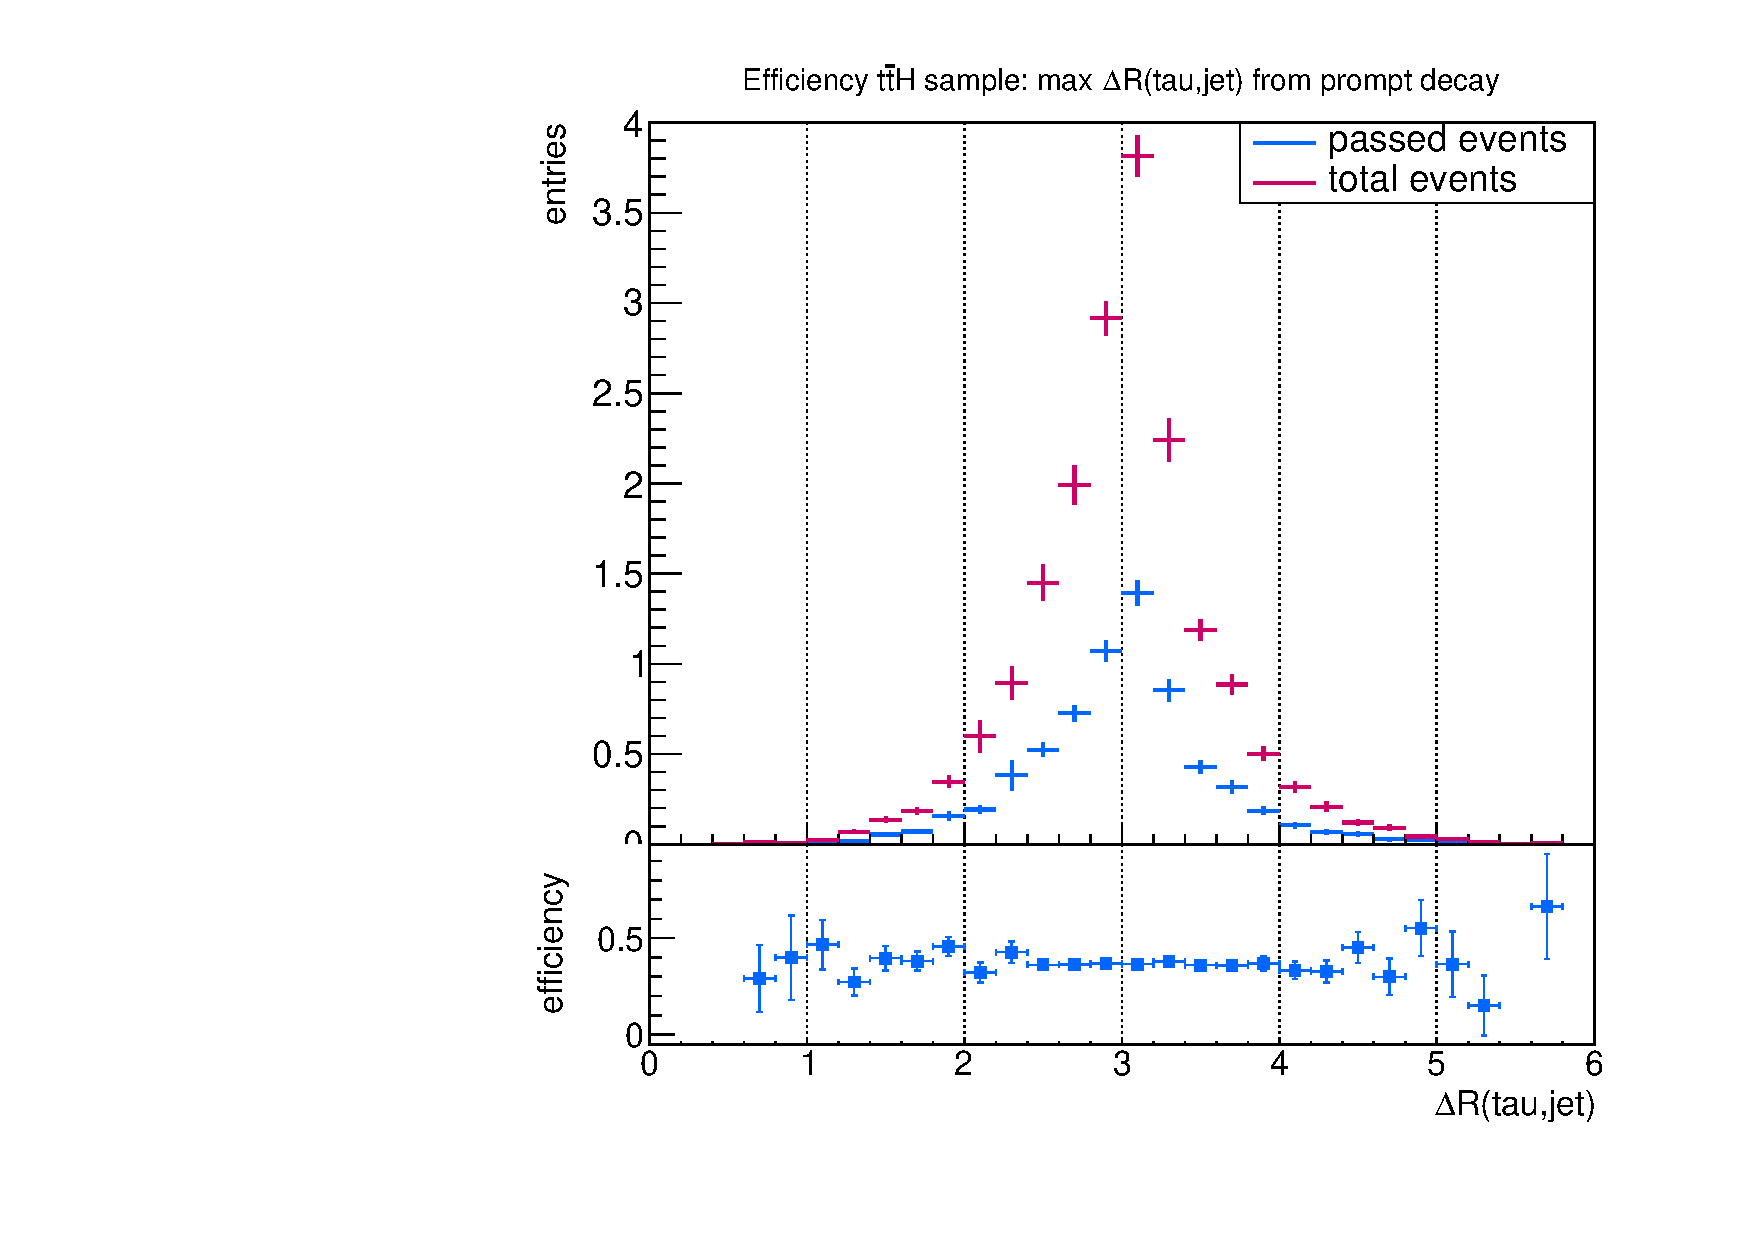
\includegraphics[width=\textwidth]{figures/plots/ttH/Divided_maxdR_pr_taujet.pdf}
                \subcaption{Maximum separation between taus originating from $W^\pm$, $Z^0$ events and b-jets.}
                \label{dR:prompt:taubjets:max}
                \end{subfigure}
\caption[Efficiency of taus originating from $W^\pm$, $Z^0$ for the separation between taus and b-jets.]{Efficiency of taus originating from $W^\pm$, $Z^0$ for the minimum and maximum separation between taus and b-jets.}
\label{dR:prompt:taubjets}
\end{figure}
%
%
\begin{figure}
  \centering
                \begin{subfigure}[t]{0.49\textwidth}
                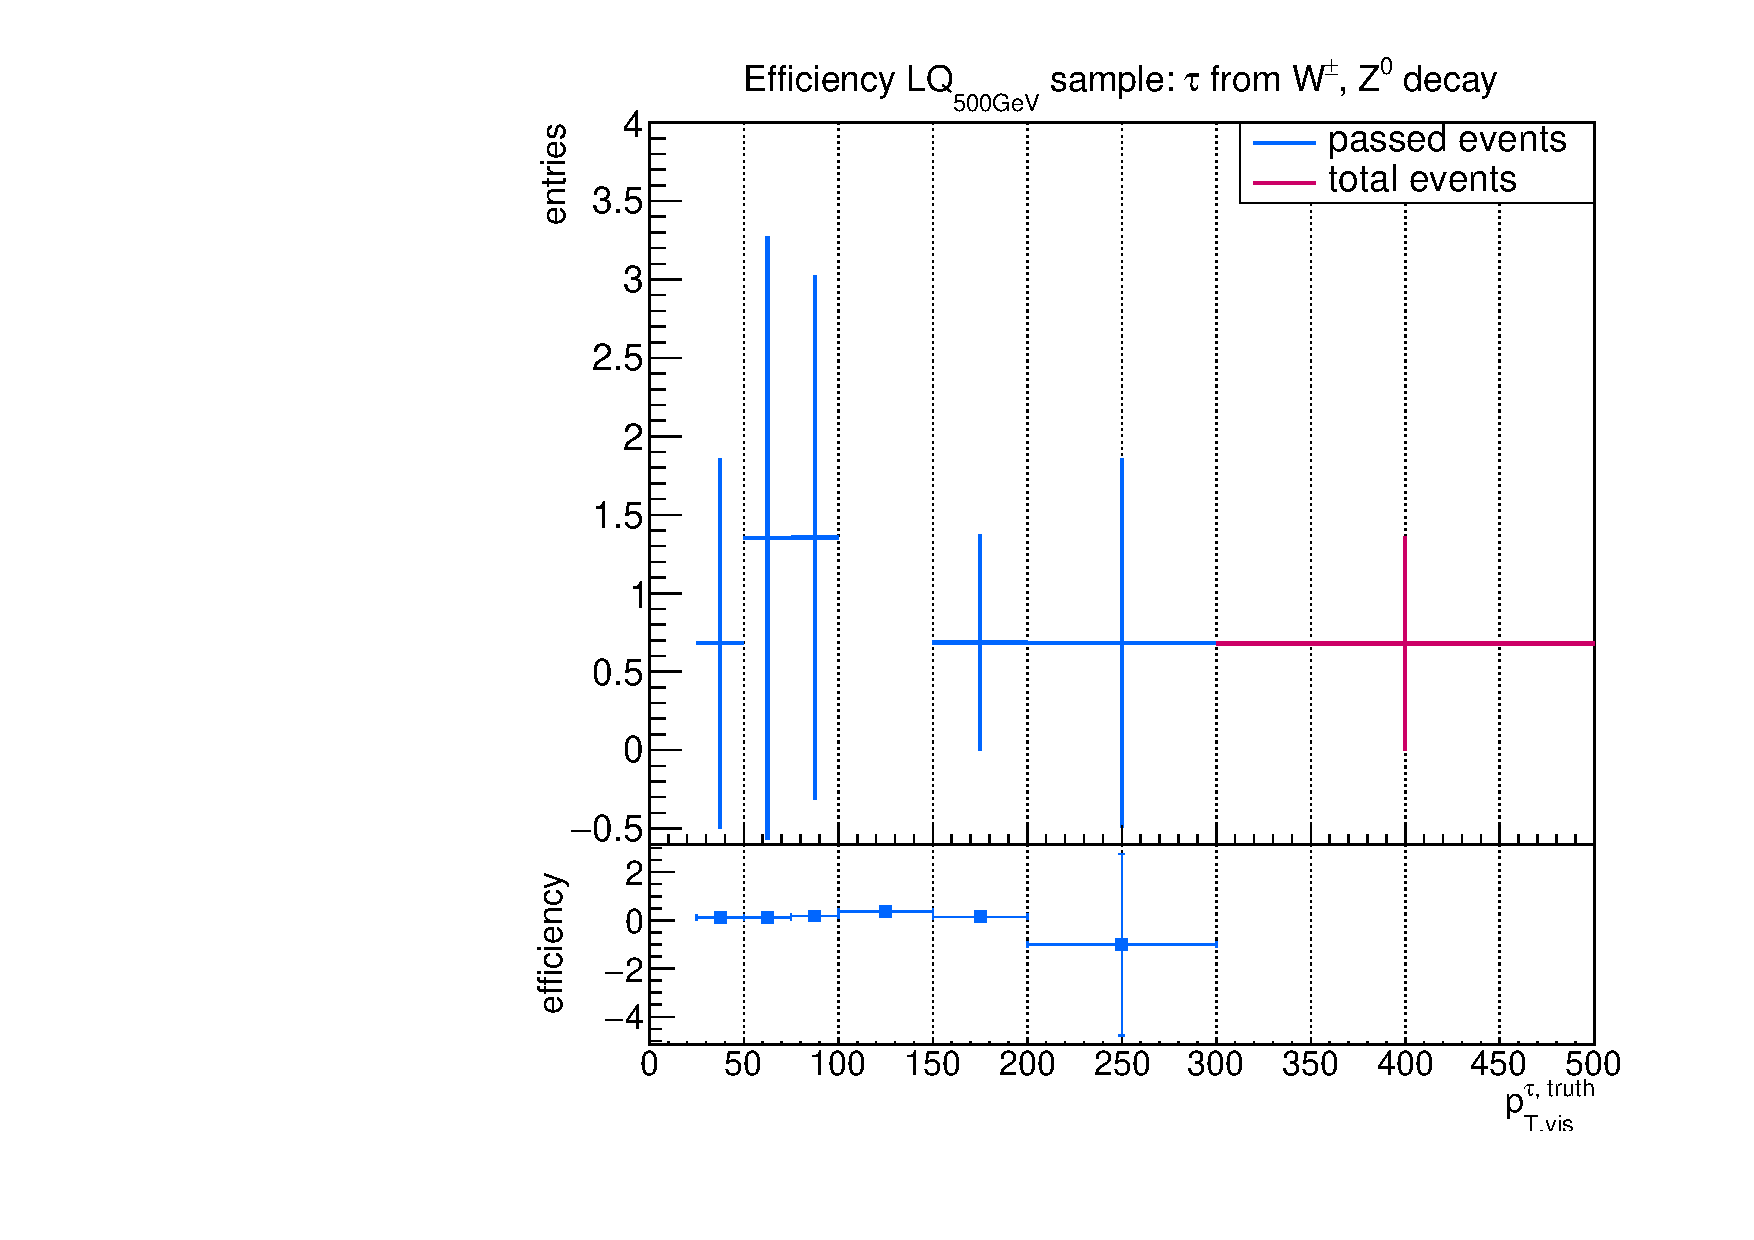
\includegraphics[width=\textwidth]{figures/plots/LQ75/Divided_prompt.pdf}
                \subcaption{Efficiency of taus originating from bosons of the weak interaction ($W^\pm$, $Z^0$) of $\SI{32.4\pm 4.4}{\percent}$ for the low mass LQ events.}
                \label{Dividedprompt:signal:allLQ75}
                \end{subfigure}
                %
                \begin{subfigure}[t]{0.49\textwidth}
                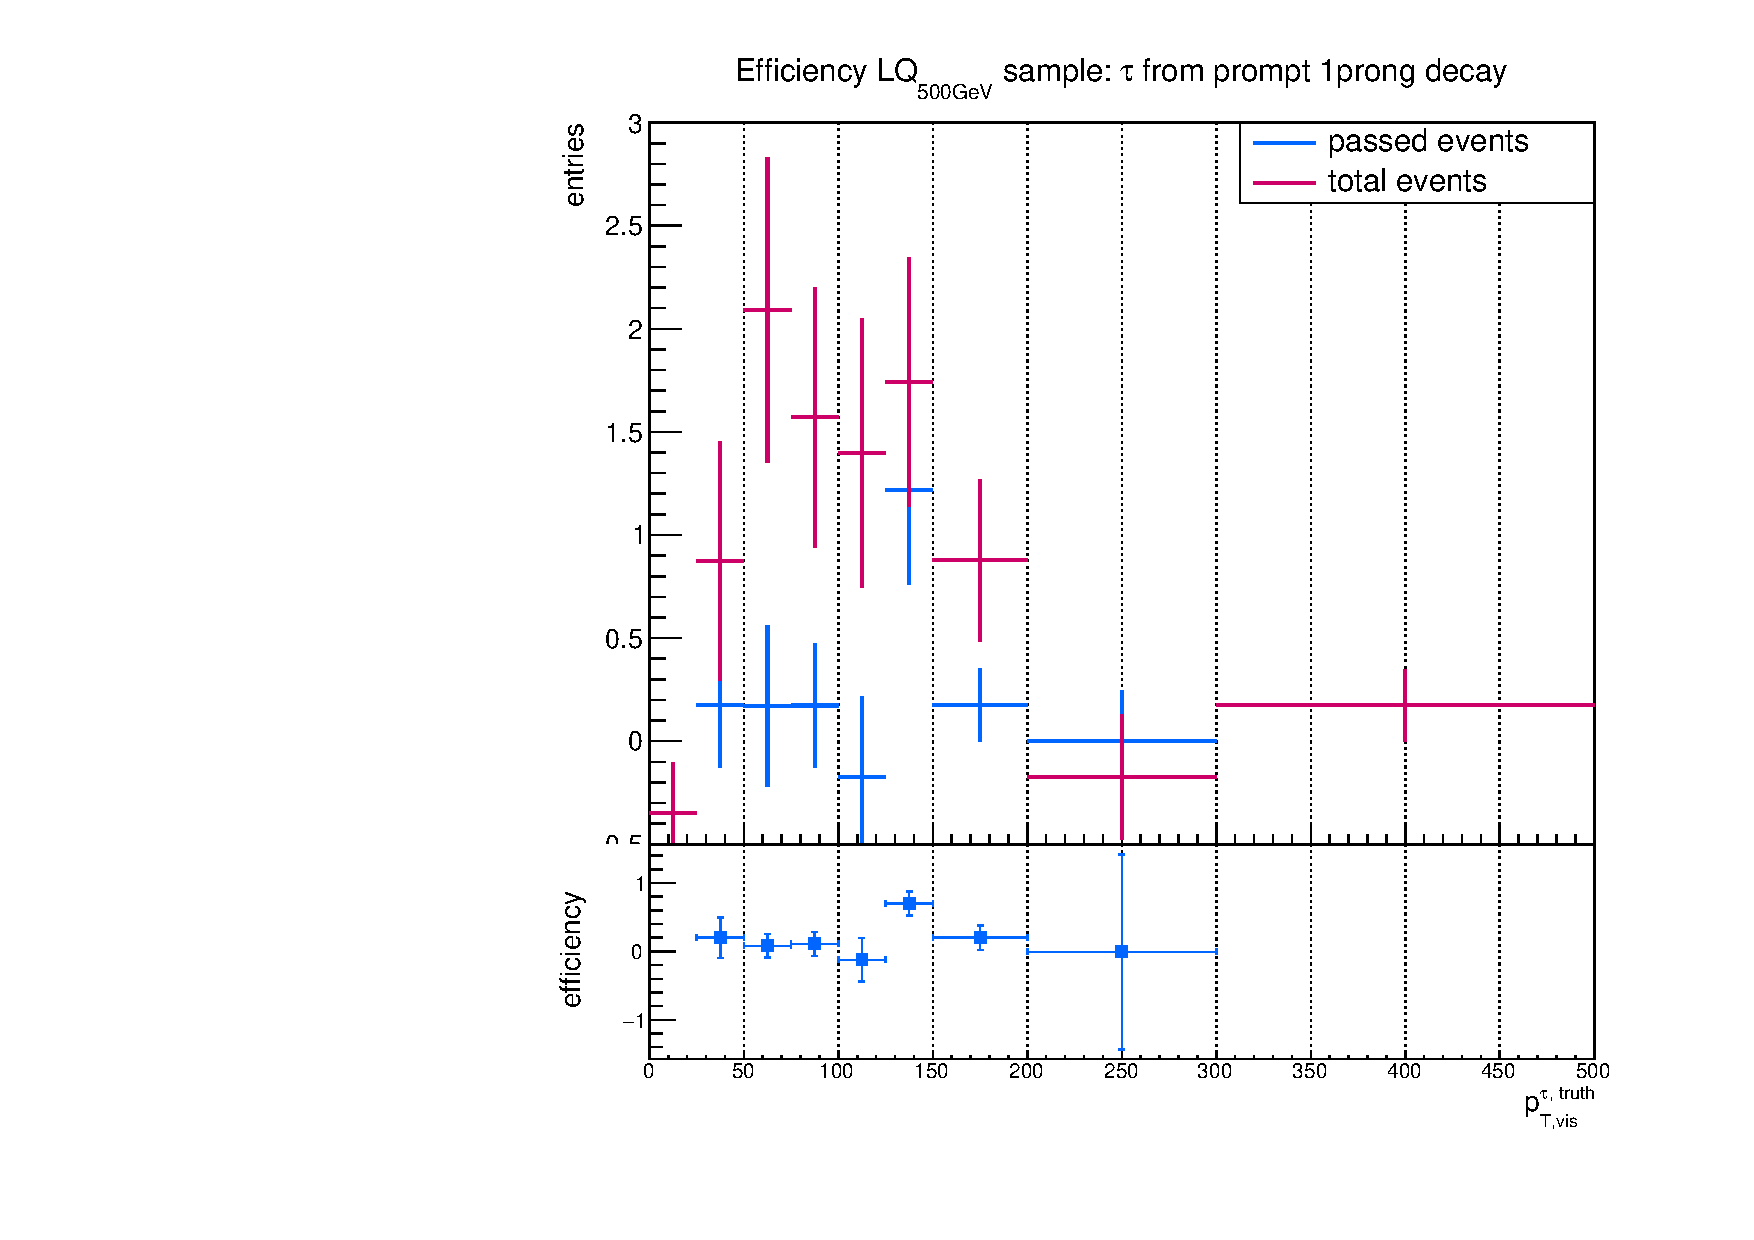
\includegraphics[width=\textwidth]{figures/plots/LQ75/Divided_prompt1prong.pdf}
                \subcaption{Efficiency of taus originating from bosons of the weak interaction ($W^\pm$, $Z^0$) and decaying in the 1-prong mode. The efficiency is $\SI{32.9\pm 5.3}{\percent}$ for the low mass LQ events.}
                \label{Dividedprompt:signal:1prongLQ75}
                \end{subfigure}
                %
                \begin{subfigure}[t]{0.49\textwidth}
                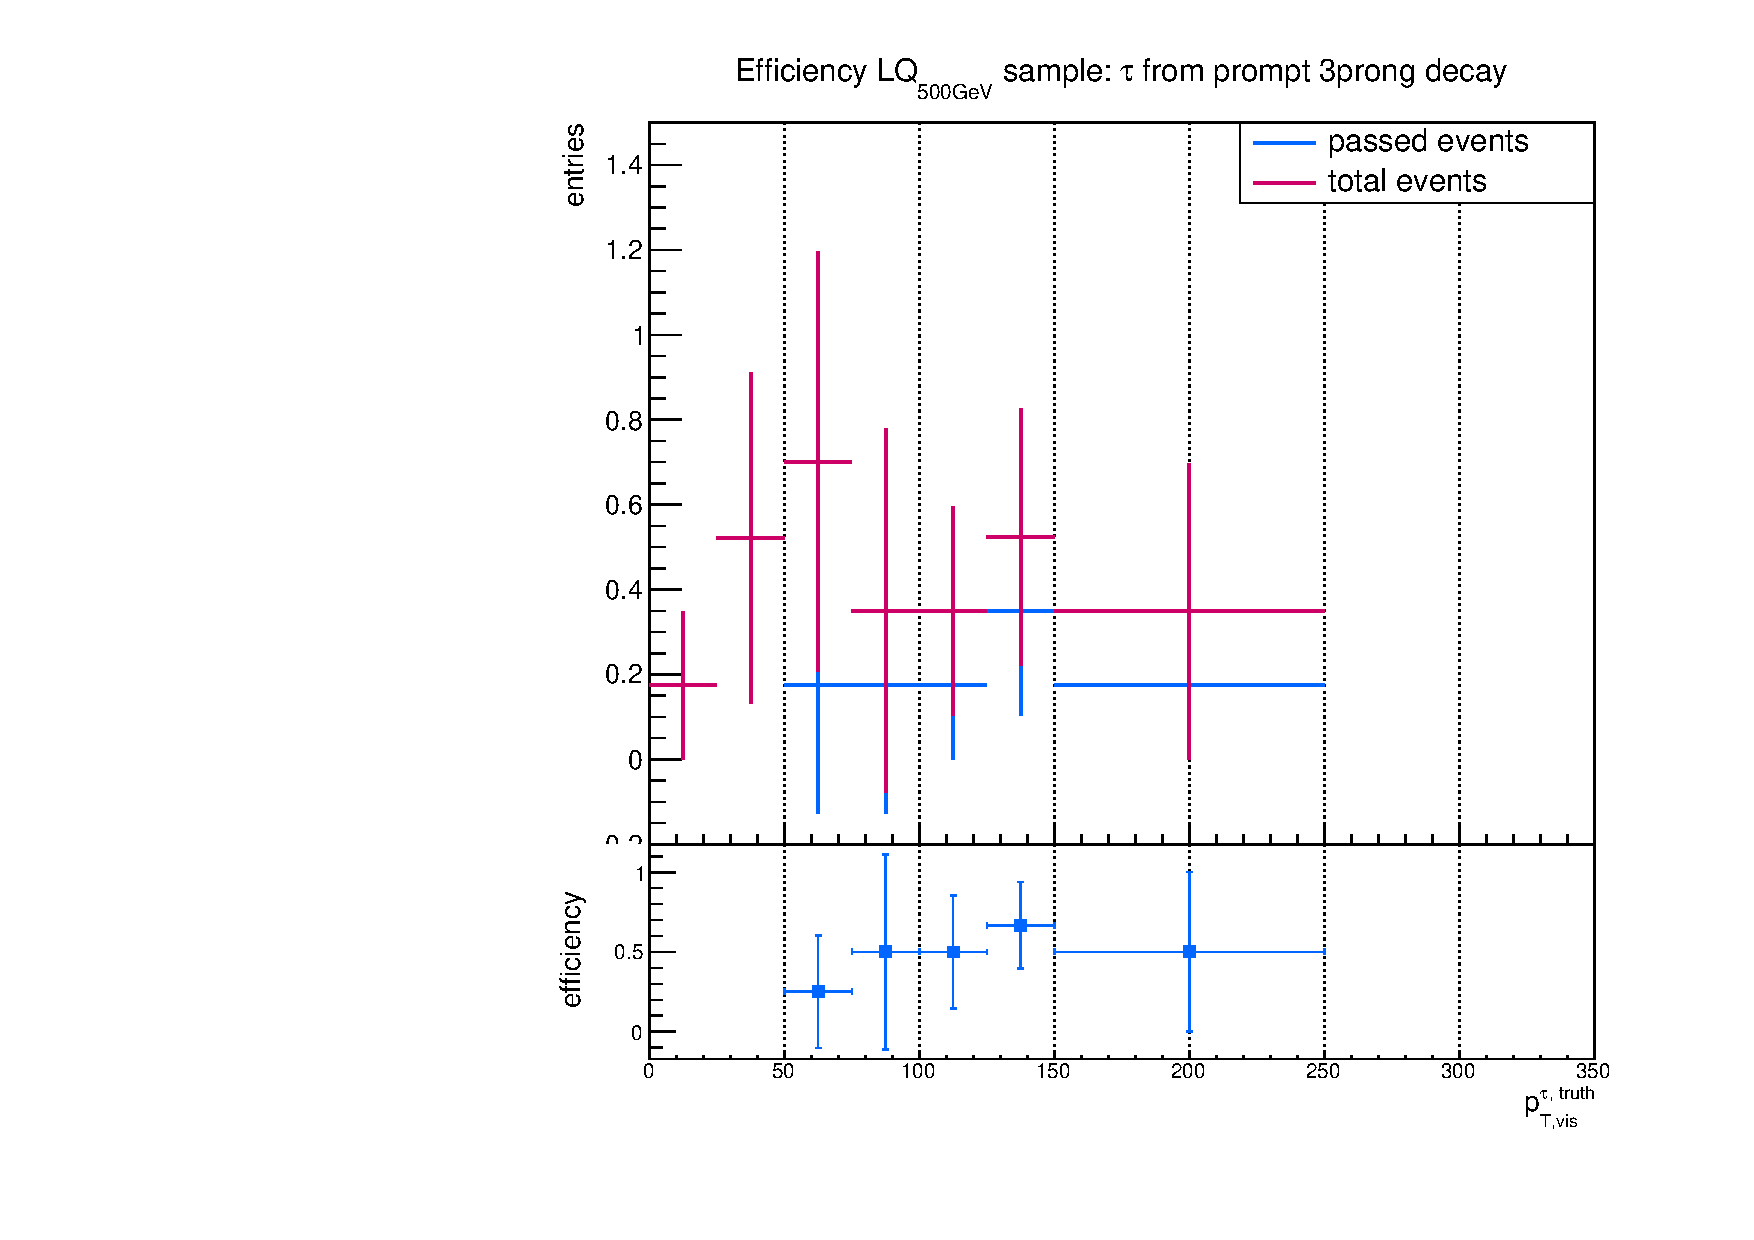
\includegraphics[width=\textwidth]{figures/plots/LQ75/Divided_prompt3prong.pdf}
                \subcaption{Efficiency of taus originating from bosons of the weak interaction ($W^\pm$, $Z^0$) and decaying in the 3-prong mode. The efficiency is $\SI{34.5\pm 8.8}{\percent}$ for the low mass LQ events.}
                \label{Dividedprompt:signal:3prongLQ75}
                \end{subfigure}
\caption[Efficiency of taus originating from bosons of the weak interaction ($W^\pm$, $Z^0$) for the low mass LQ signal events.]{Efficiency of taus originating from bosons of the weak interaction ($W^\pm$, $Z^0$) for the low mass LQ signal events. The efficiency is defined as the number of taus passing the basic selection and matched to a hadronic truth tau as well as the origin is from a $W^\pm$ or $Z^0$ boson over the total number of taus passing the basic selection and originating from a $W^\pm$ or $Z^0$ boson.}
\label{Dividedprompt:signal:LQ75}
\end{figure}


\begin{figure}
  \centering
                \begin{subfigure}[t]{0.49\textwidth}
                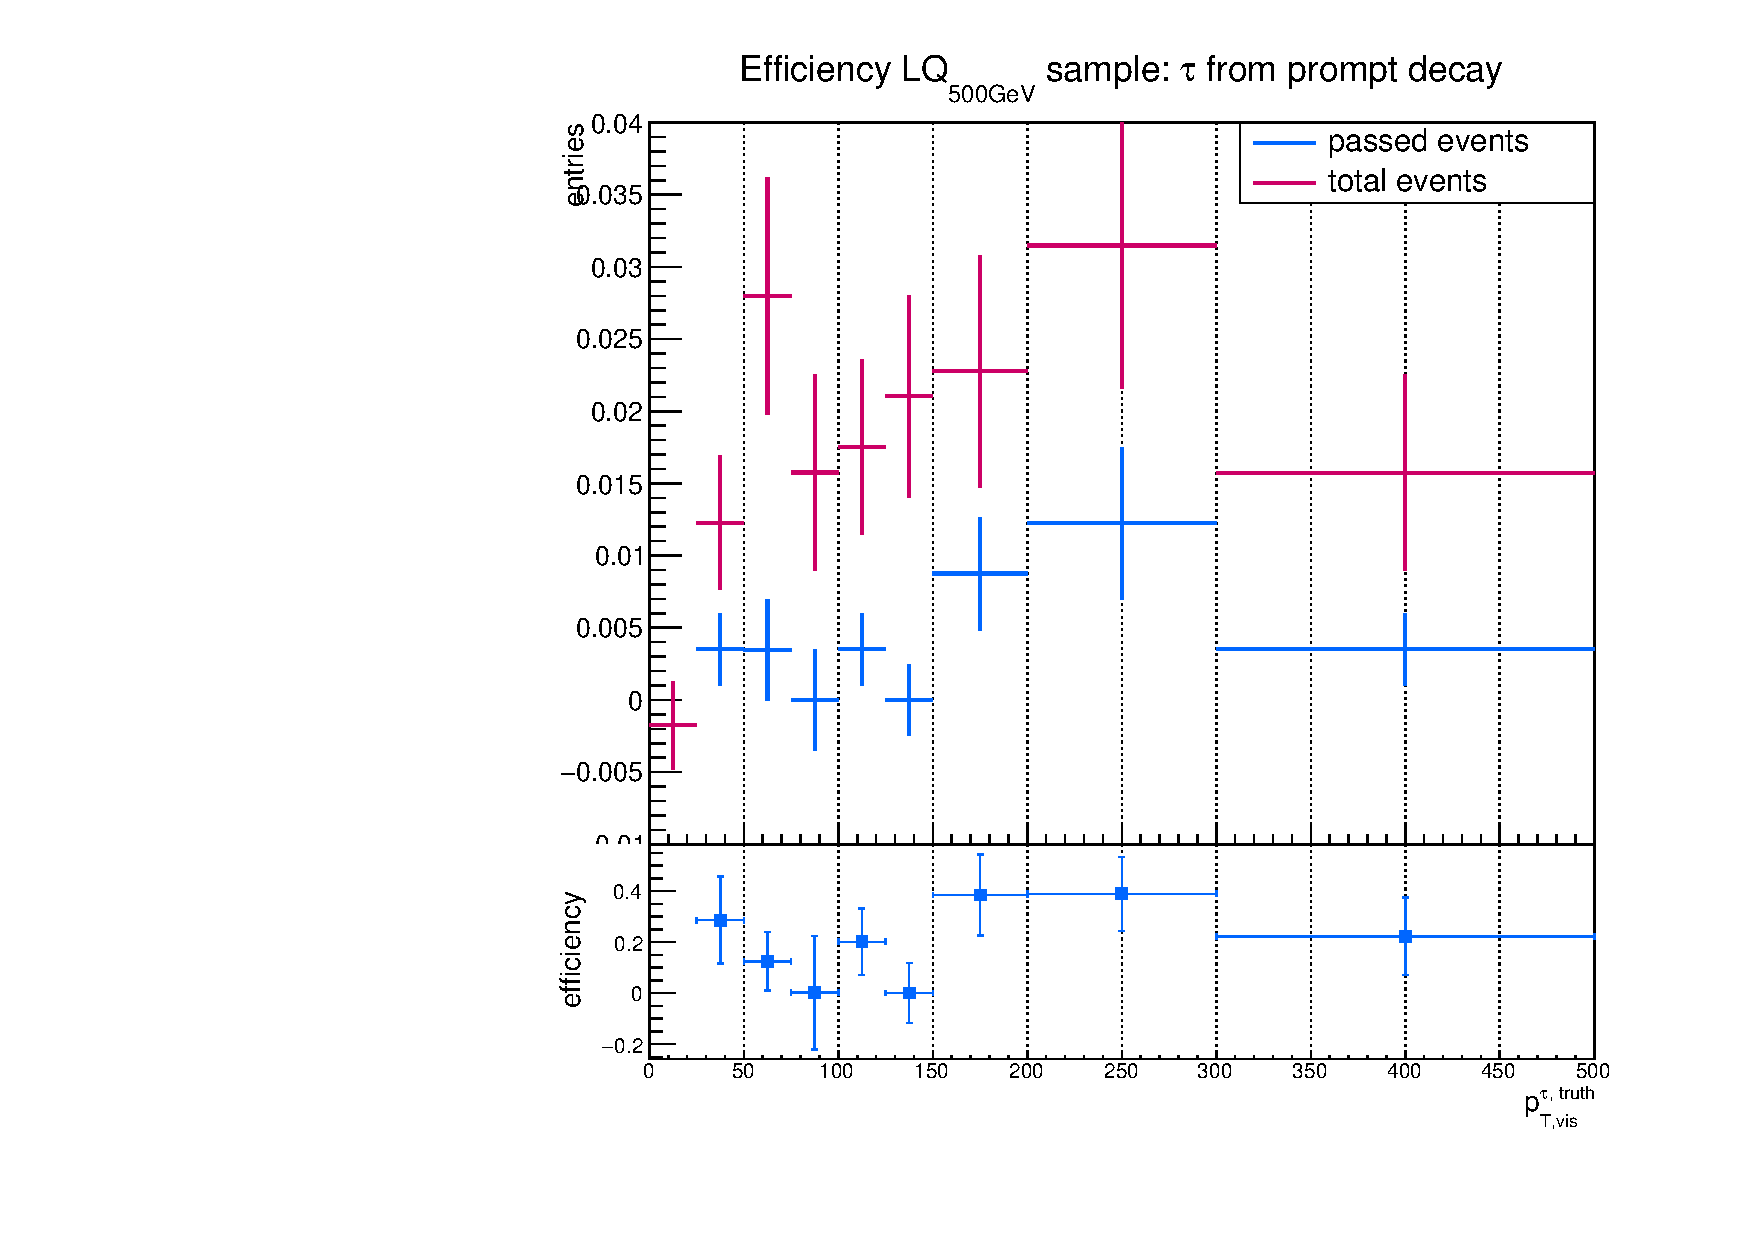
\includegraphics[width=\textwidth]{figures/plots/LQ76/Divided_prompt.pdf}
                \subcaption{Efficiency of taus originating from bosons of the weak interaction ($W^\pm$, $Z^0$) of $\SI{20.8\pm 3.3}{\percent}$ for the high mass LQ events.}
                \label{Dividedprompt:signal:allLQ76}
                \end{subfigure}
                %
                \begin{subfigure}[t]{0.49\textwidth}
                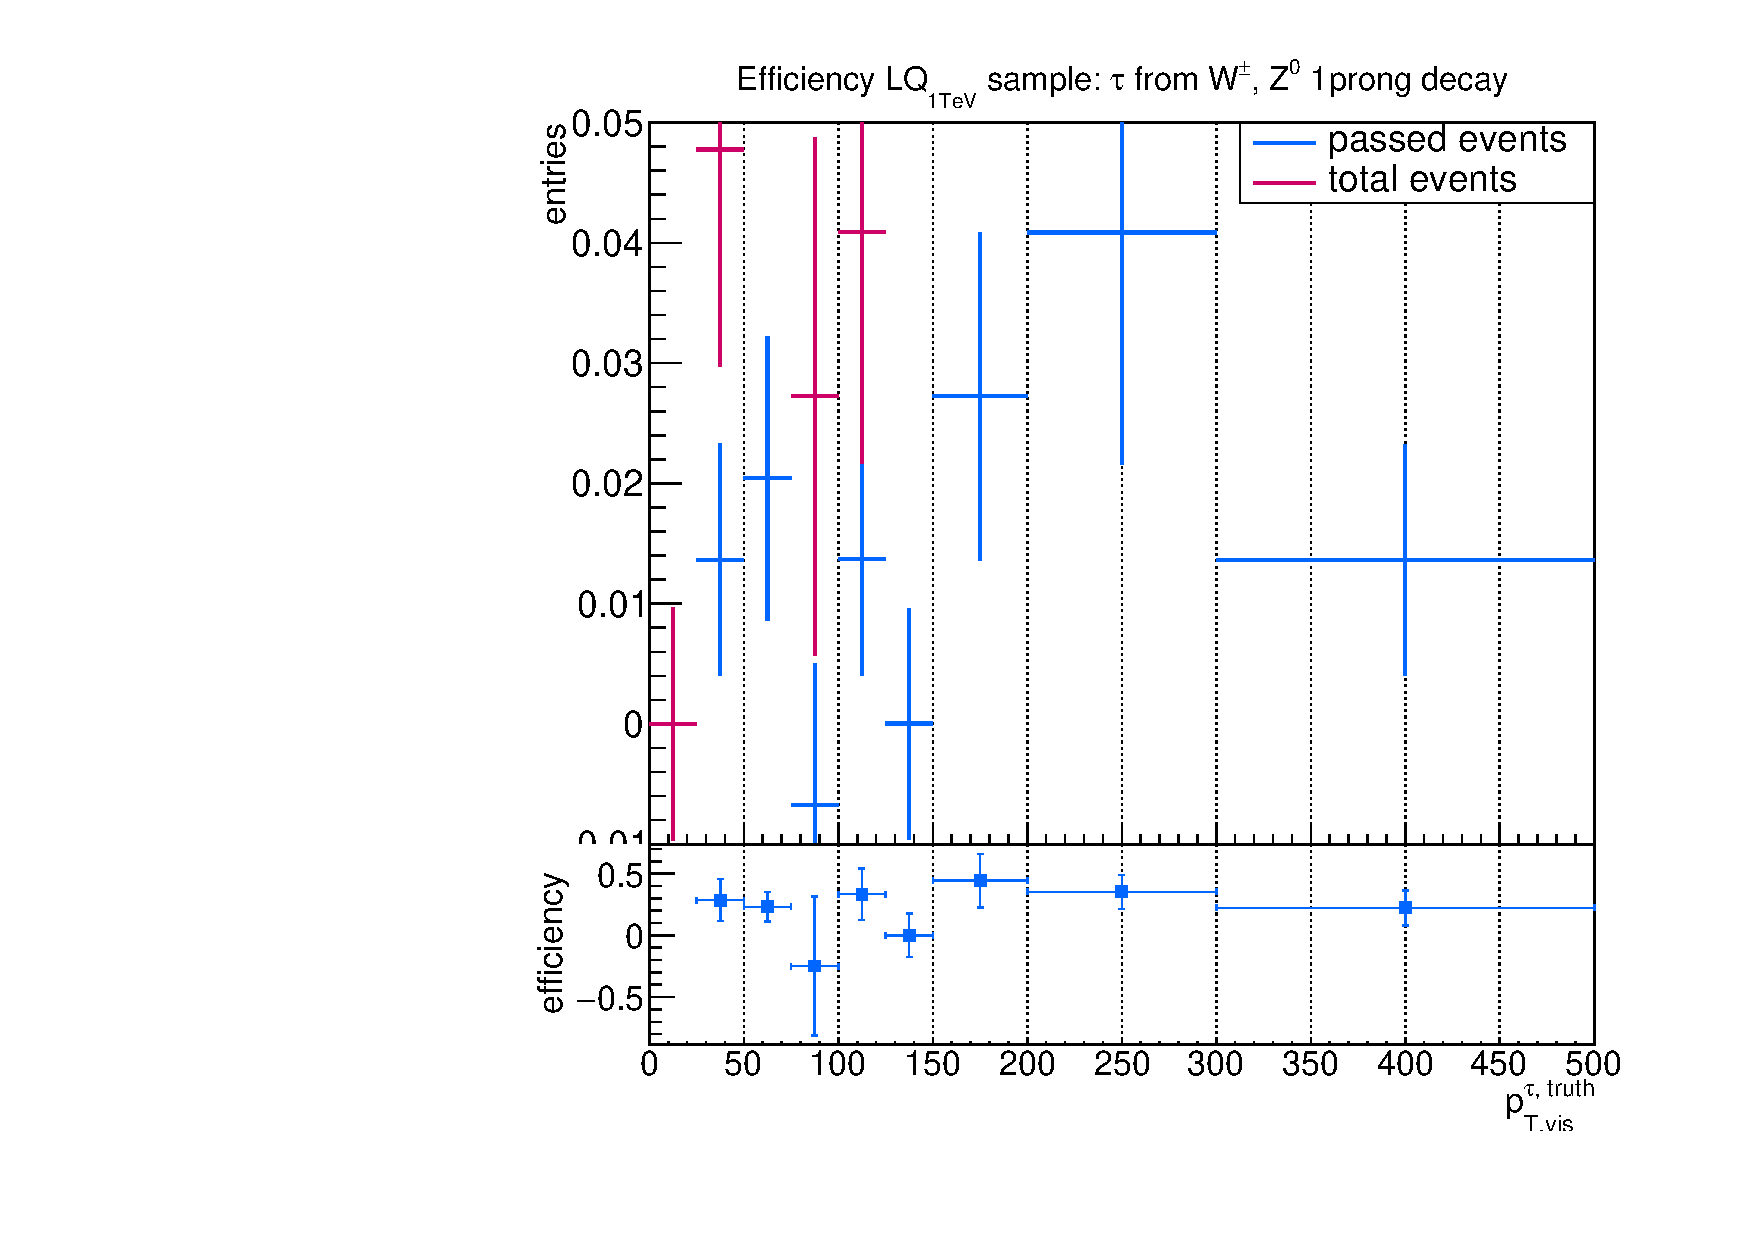
\includegraphics[width=\textwidth]{figures/plots/LQ76/Divided_prompt1prong.pdf}
                \subcaption{Efficiency of taus originating from bosons of the weak interaction ($W^\pm$, $Z^0$) and decaying in the 1-prong mode. The efficiency is $\SI{23.6\pm 4.1}{\percent}$ for the high mass LQ events.}
                \label{Dividedprompt:signal:1prongLQ76}
                \end{subfigure}
                %
                \begin{subfigure}[t]{0.49\textwidth}
                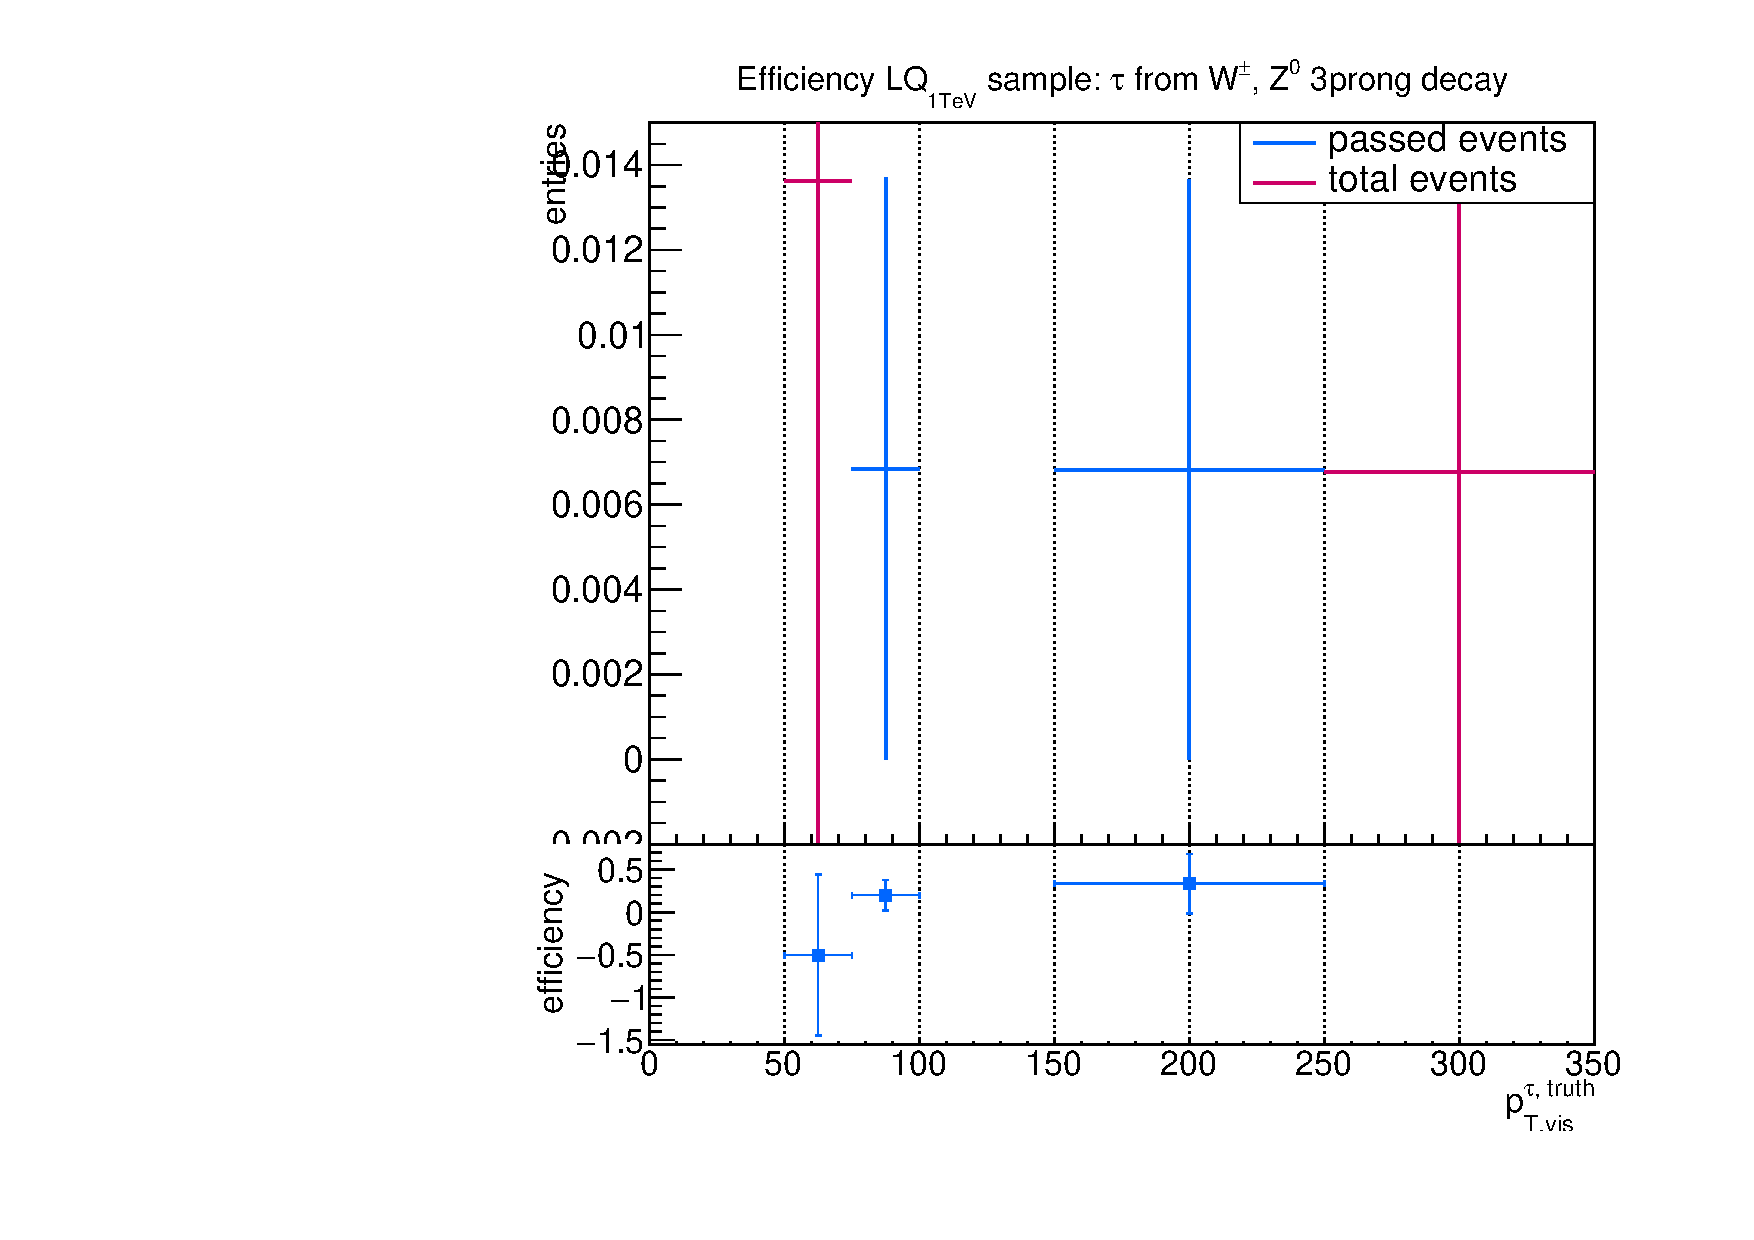
\includegraphics[width=\textwidth]{figures/plots/LQ76/Divided_prompt3prong.pdf}
                \subcaption{Efficiency of taus originating from bosons of the weak interaction ($W^\pm$, $Z^0$) and decaying in the 3-prong mode. The efficiency is $\SI{12.5\pm 5.8}{\percent}$ for the high mass LQ events.}
                \label{Dividedprompt:signal:3prongLQ76}
                \end{subfigure}            
\caption[Efficiency of taus originating from bosons of the weak interaction ($W^\pm$, $Z^0$) for the high mass LQ signal events.]{Efficiency of taus originating from bosons of the weak interaction ($W^\pm$, $Z^0$) for the high mass LQ signal events. The efficiency is defined as the number of taus passing the basic selection and matched to a hadronic truth tau as well as the origin is from a $W^\pm$ or $Z^0$ boson over the total number of taus passing the basic selection and originating from a $W^\pm$ or $Z^0$ boson.}
\label{Dividedprompt:signal:LQ76}
\end{figure}
%
%
\begin{figure}
  \centering    
                \begin{subfigure}[t]{0.49\textwidth}
                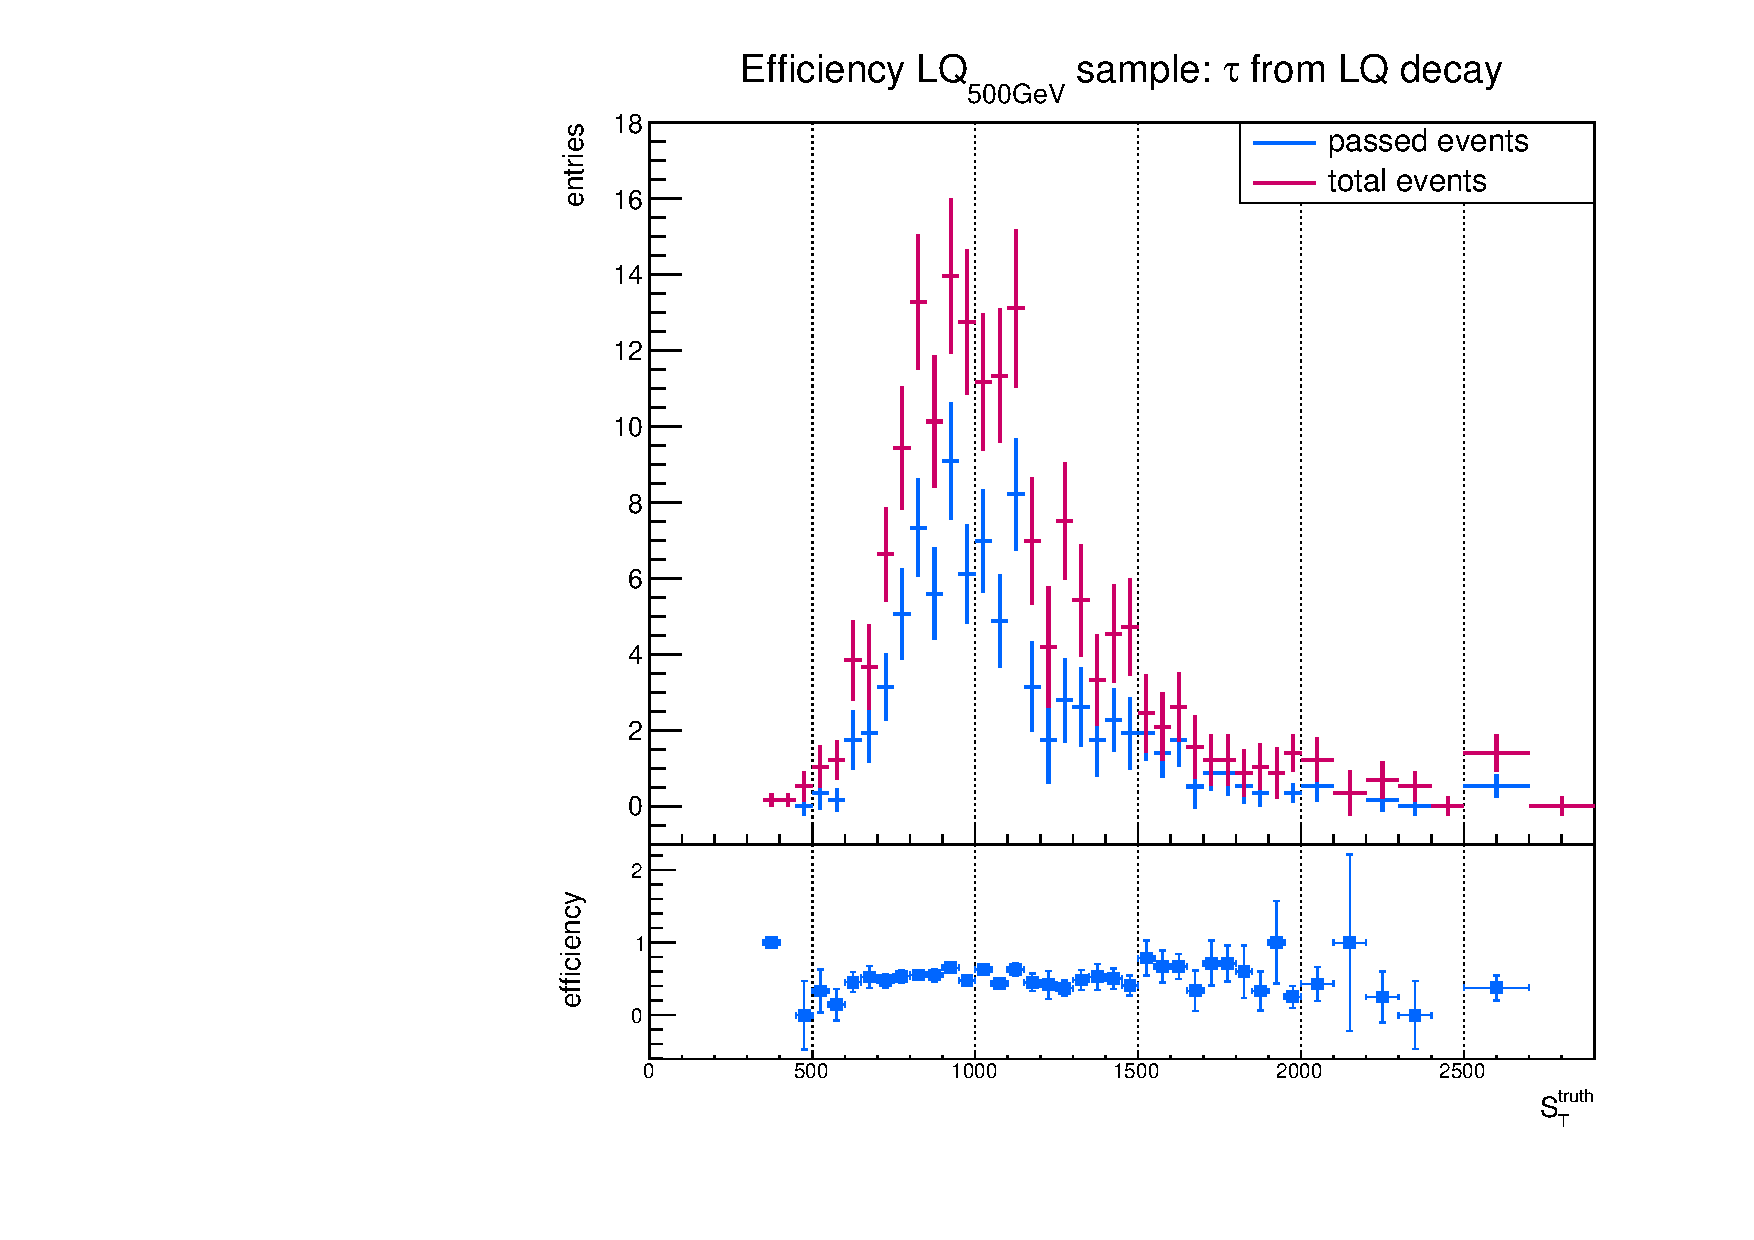
\includegraphics[width=\textwidth]{figures/plots/LQ75/Divided_fromLQST.pdf}
                \subcaption{Efficiency of taus originating from $W^\pm$ and $Z^0$ bosons of depending on $S_{T}$ low mass LQ sample.}
                \label{Dividedprompt:signal:STLQ75}
                \end{subfigure}
                %
                \begin{subfigure}[t]{0.49\textwidth}
                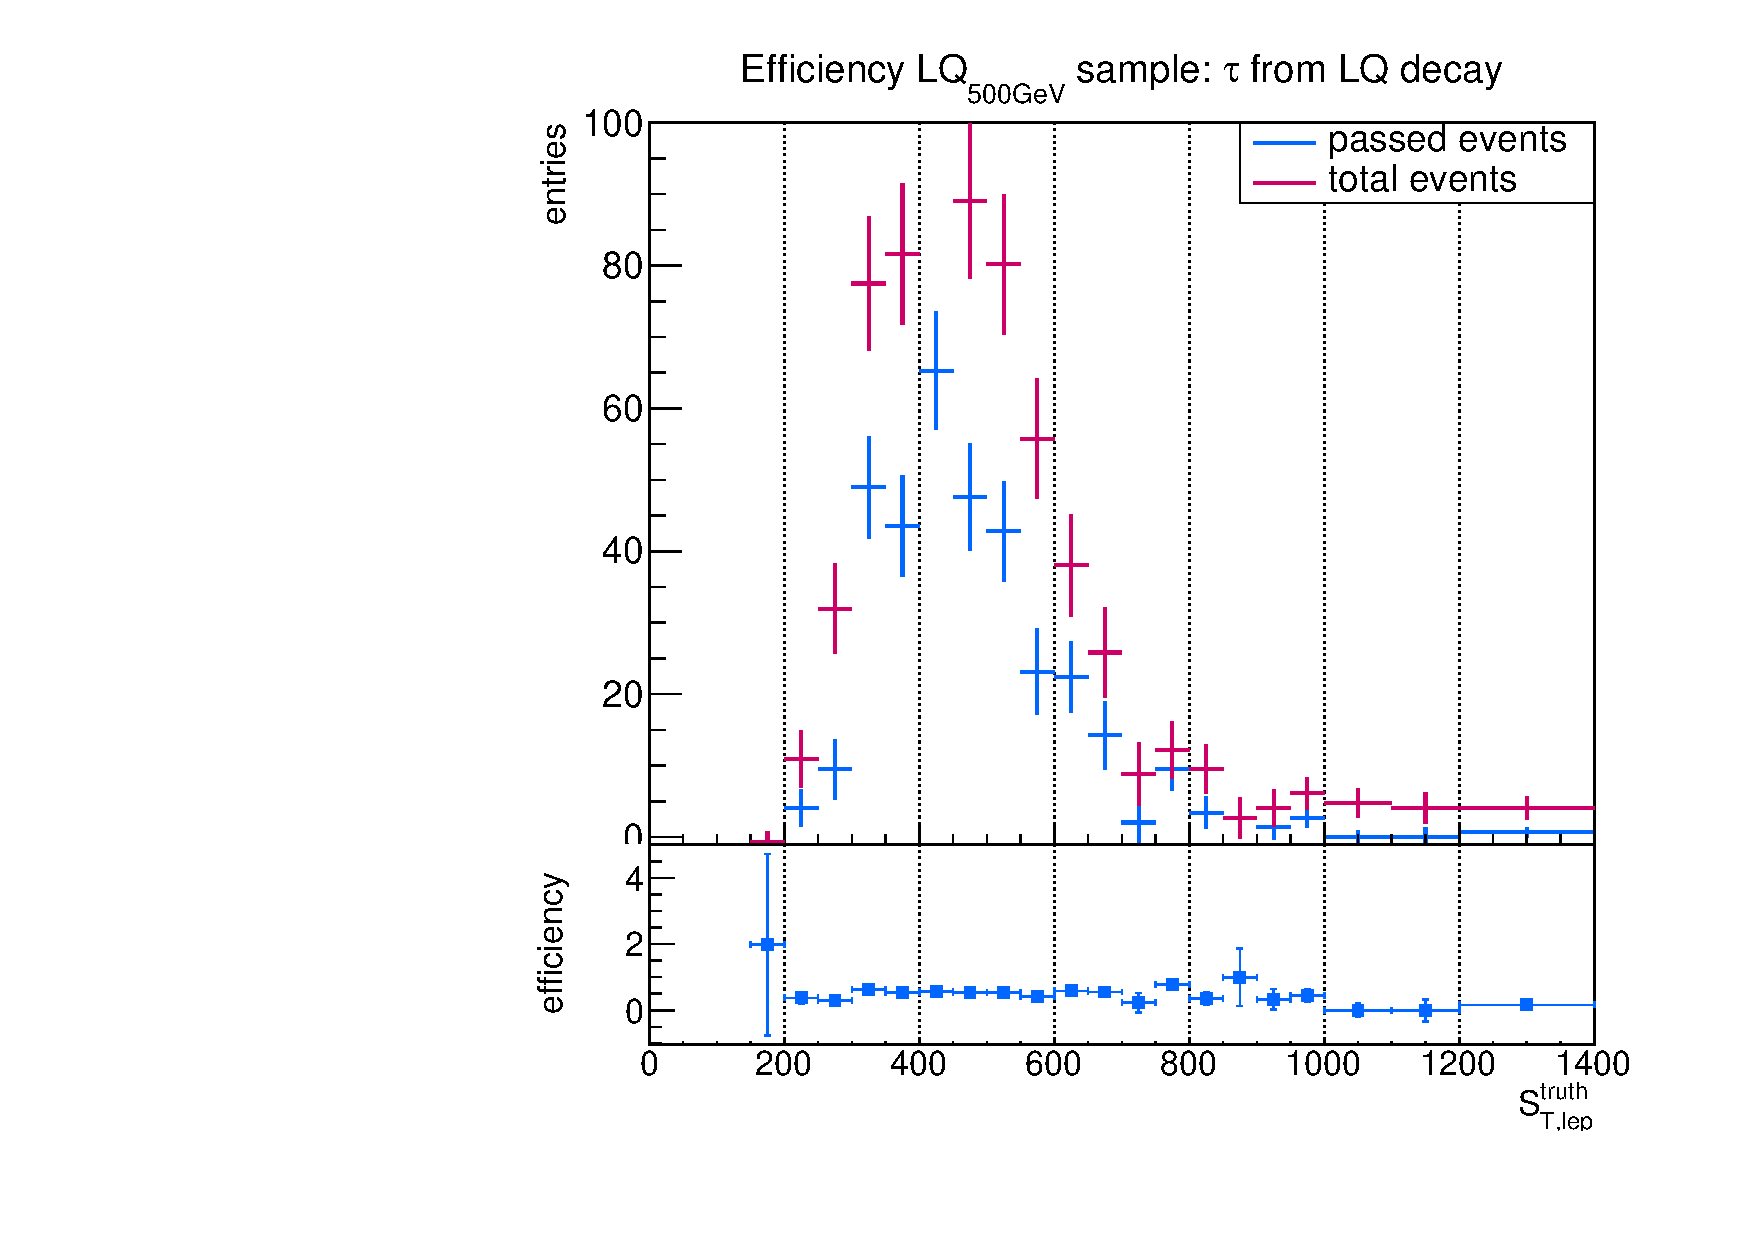
\includegraphics[width=\textwidth]{figures/plots/LQ75/Divided_fromLQSTlep.pdf}
                \subcaption{Efficiency of taus originating from $W^\pm$ and $Z^0$ bosons of depending on $S_{T,\text{lep}}$ low mass LQ sample.}
                \label{Dividedprompt:signal:STlepLQ75}
                \end{subfigure}
                %
                \begin{subfigure}[t]{0.49\textwidth}
                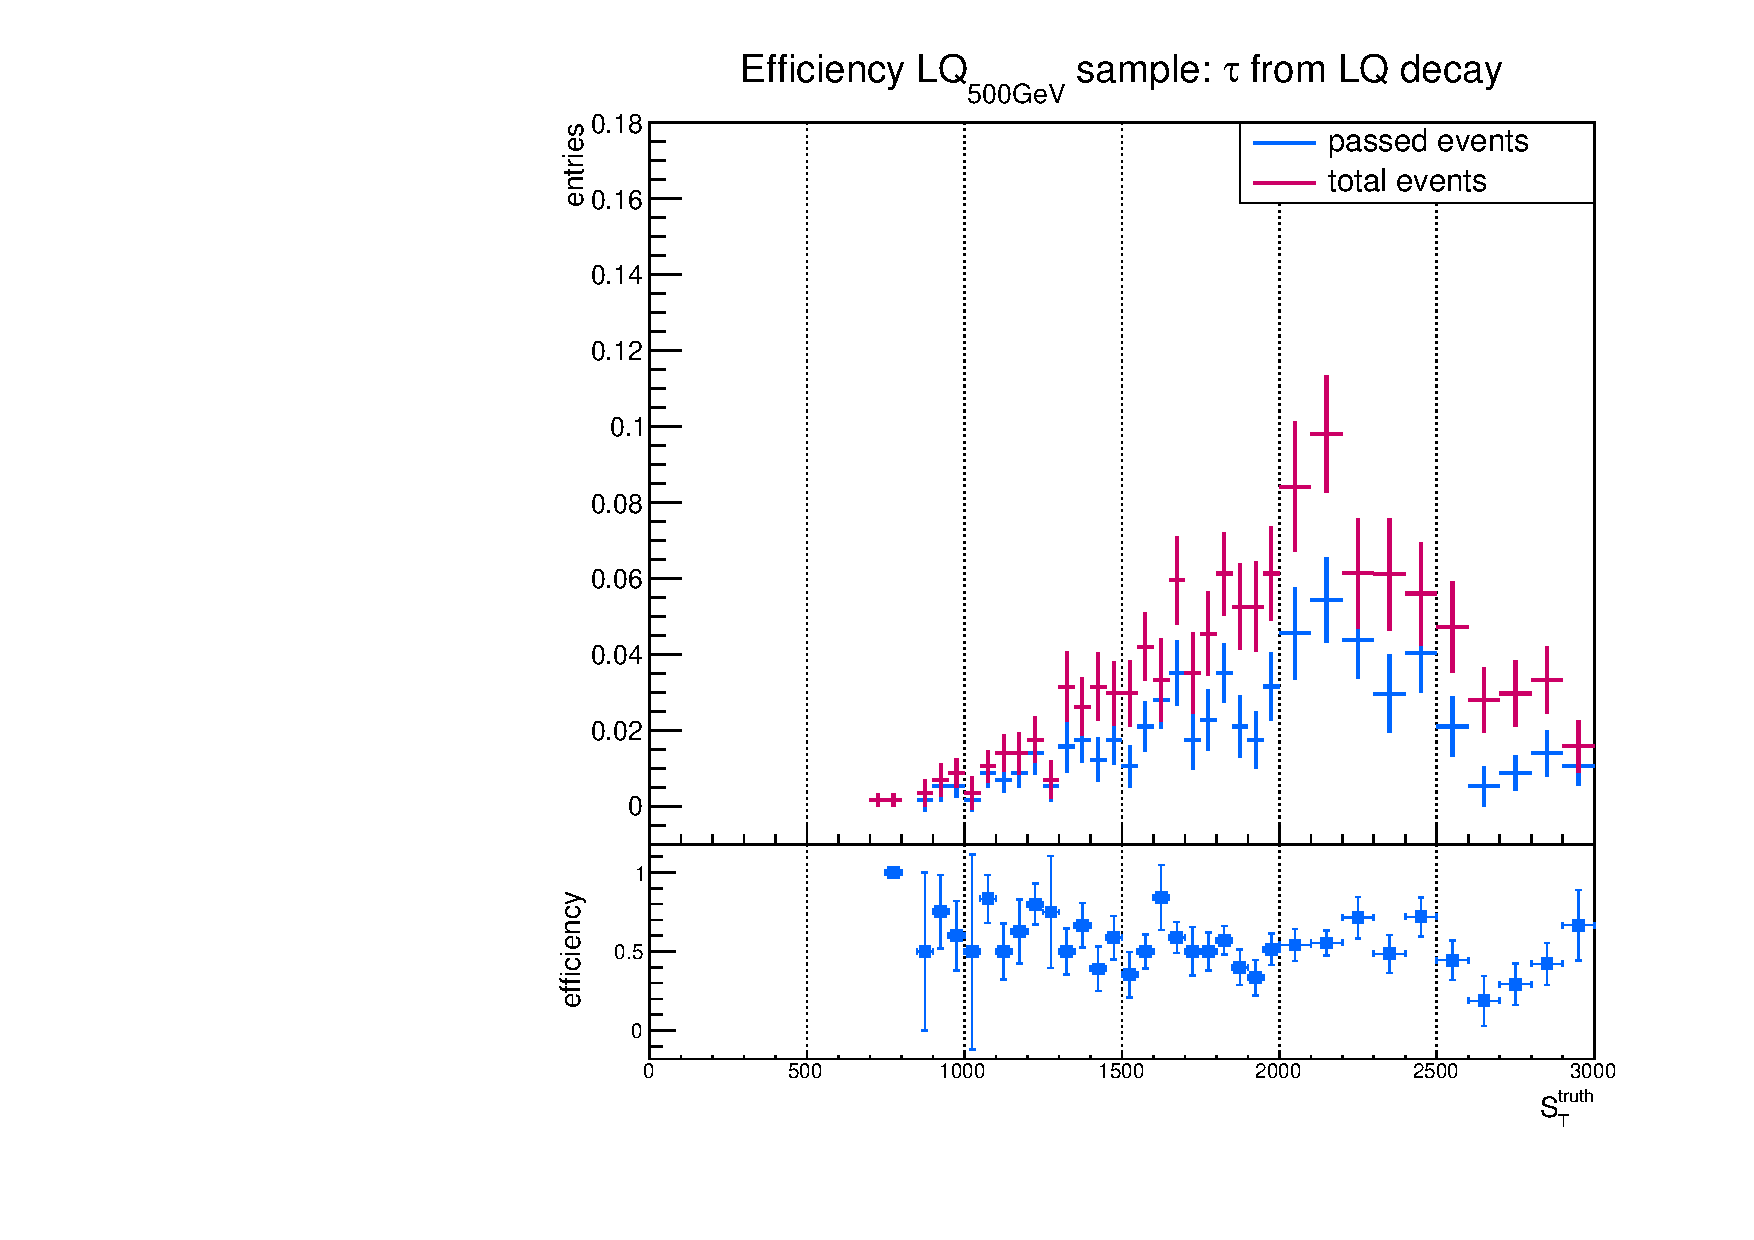
\includegraphics[width=\textwidth]{figures/plots/LQ76/Divided_fromLQST.pdf}
                \subcaption{Efficiency of taus originating from $W^\pm$ and $Z^0$ bosons of depending on $S_{T}$ high mass LQ sample.}
                \label{Dividedprompt:signal:STLQ76}
                \end{subfigure}
                %
                \begin{subfigure}[t]{0.49\textwidth}
                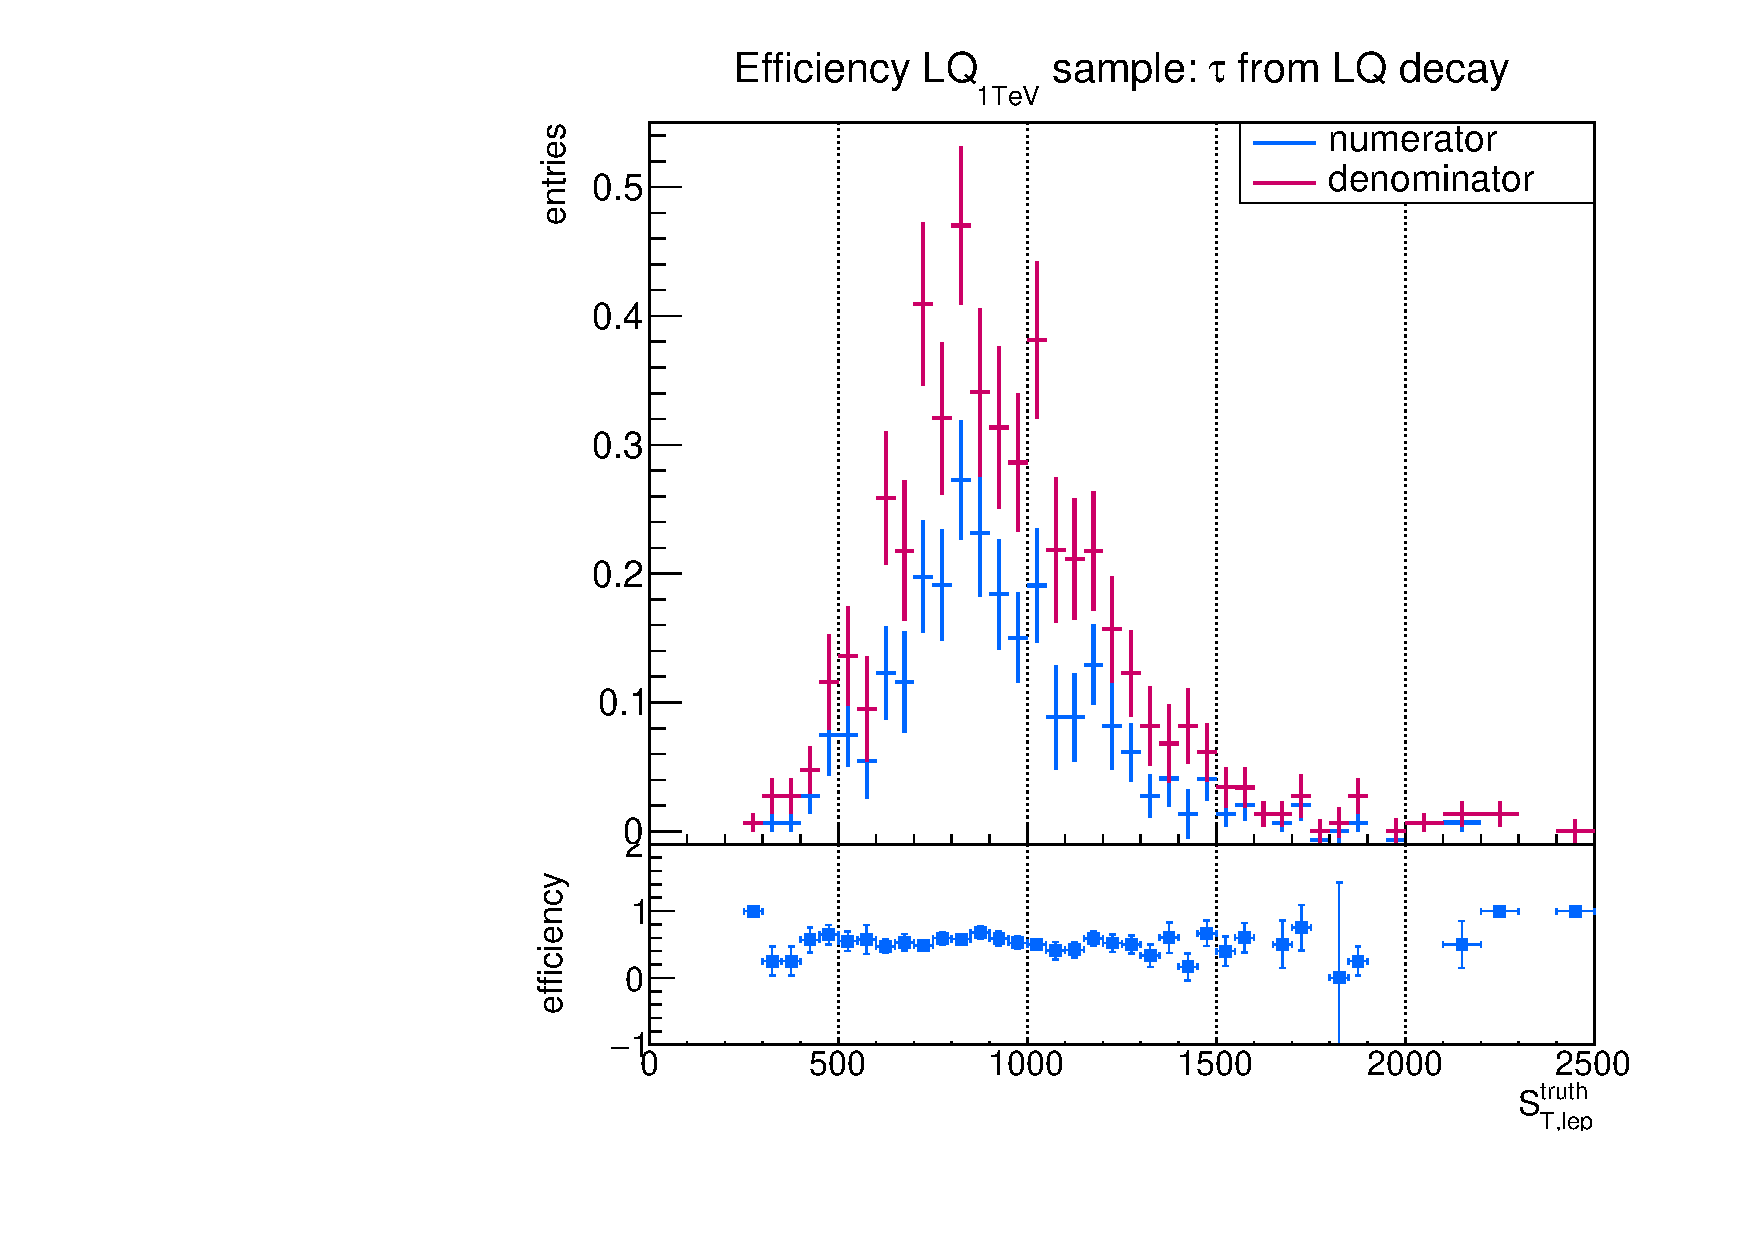
\includegraphics[width=\textwidth]{figures/plots/LQ76/Divided_fromLQSTlep.pdf}
                \subcaption{Efficiency of taus originating from $W^\pm$ and $Z^0$ bosons of depending on $S_{T,\text{lep}}$ high mass LQ sample.}
                \label{Dividedprompt:signal:STlepLQ76}
                \end{subfigure}
\caption[Efficiency of taus originating from $W^\pm$ and $Z^0$ bosons for the LQ signal events.]{Efficiency of taus originating from $W^\pm$ and $Z^0$ bosons depending on $S_{T}$ (a), (c) and $S_{T,\text{lep}}$ (b), (d) for the LQ signal events.}
\label{Dividedprompt:signal:STgedöns}
\end{figure}
%
%
\begin{figure}
  \centering
                \begin{subfigure}[t]{0.49\textwidth}
                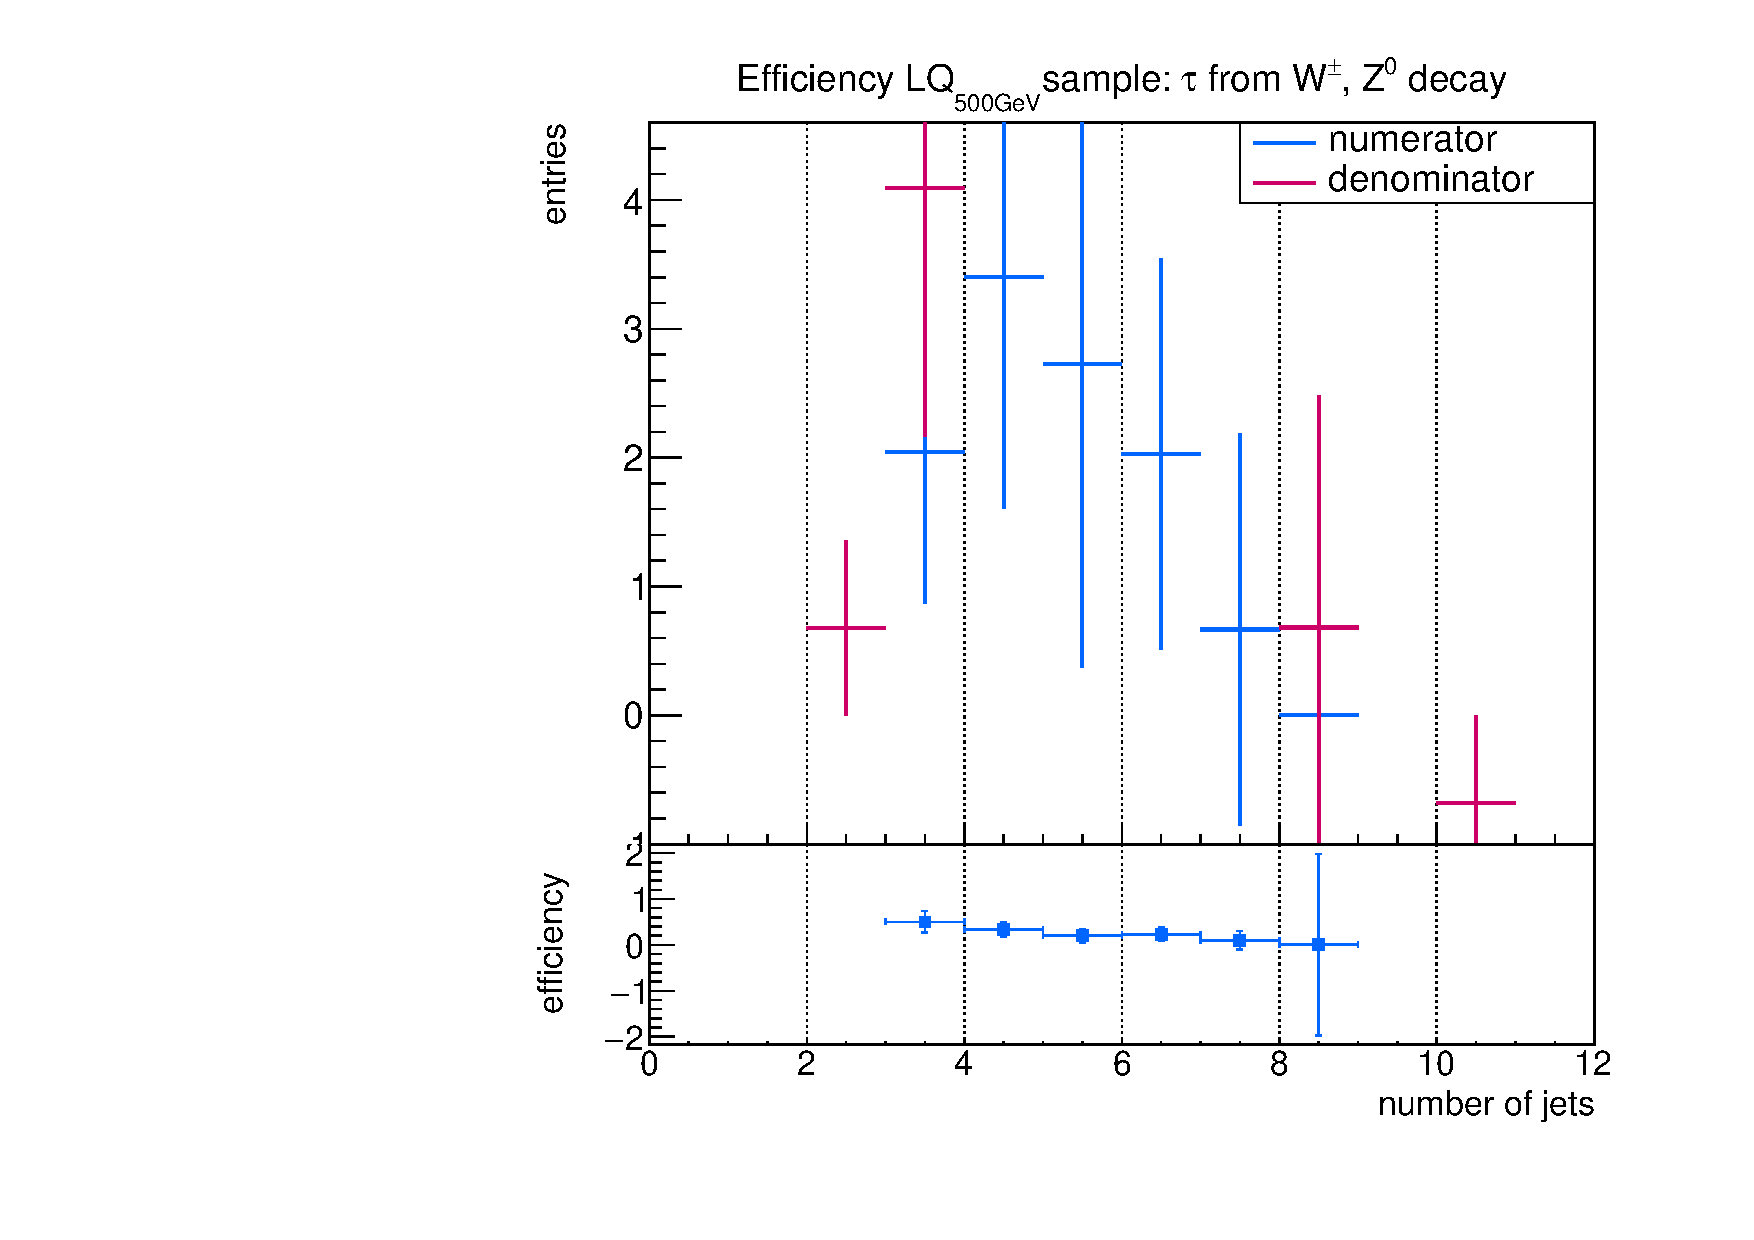
\includegraphics[width=\textwidth]{figures/plots/LQ75/Divided_promptnjets.pdf}
                \subcaption{Efficiency of taus originating from $W^\pm$, and $Z^0$ bosons depending on the number of jets for the LQ sample with low mass point.}
                \label{Dividedprompt:signal:njetsLQ75}
                \end{subfigure}
                %
                \begin{subfigure}[t]{0.49\textwidth}
                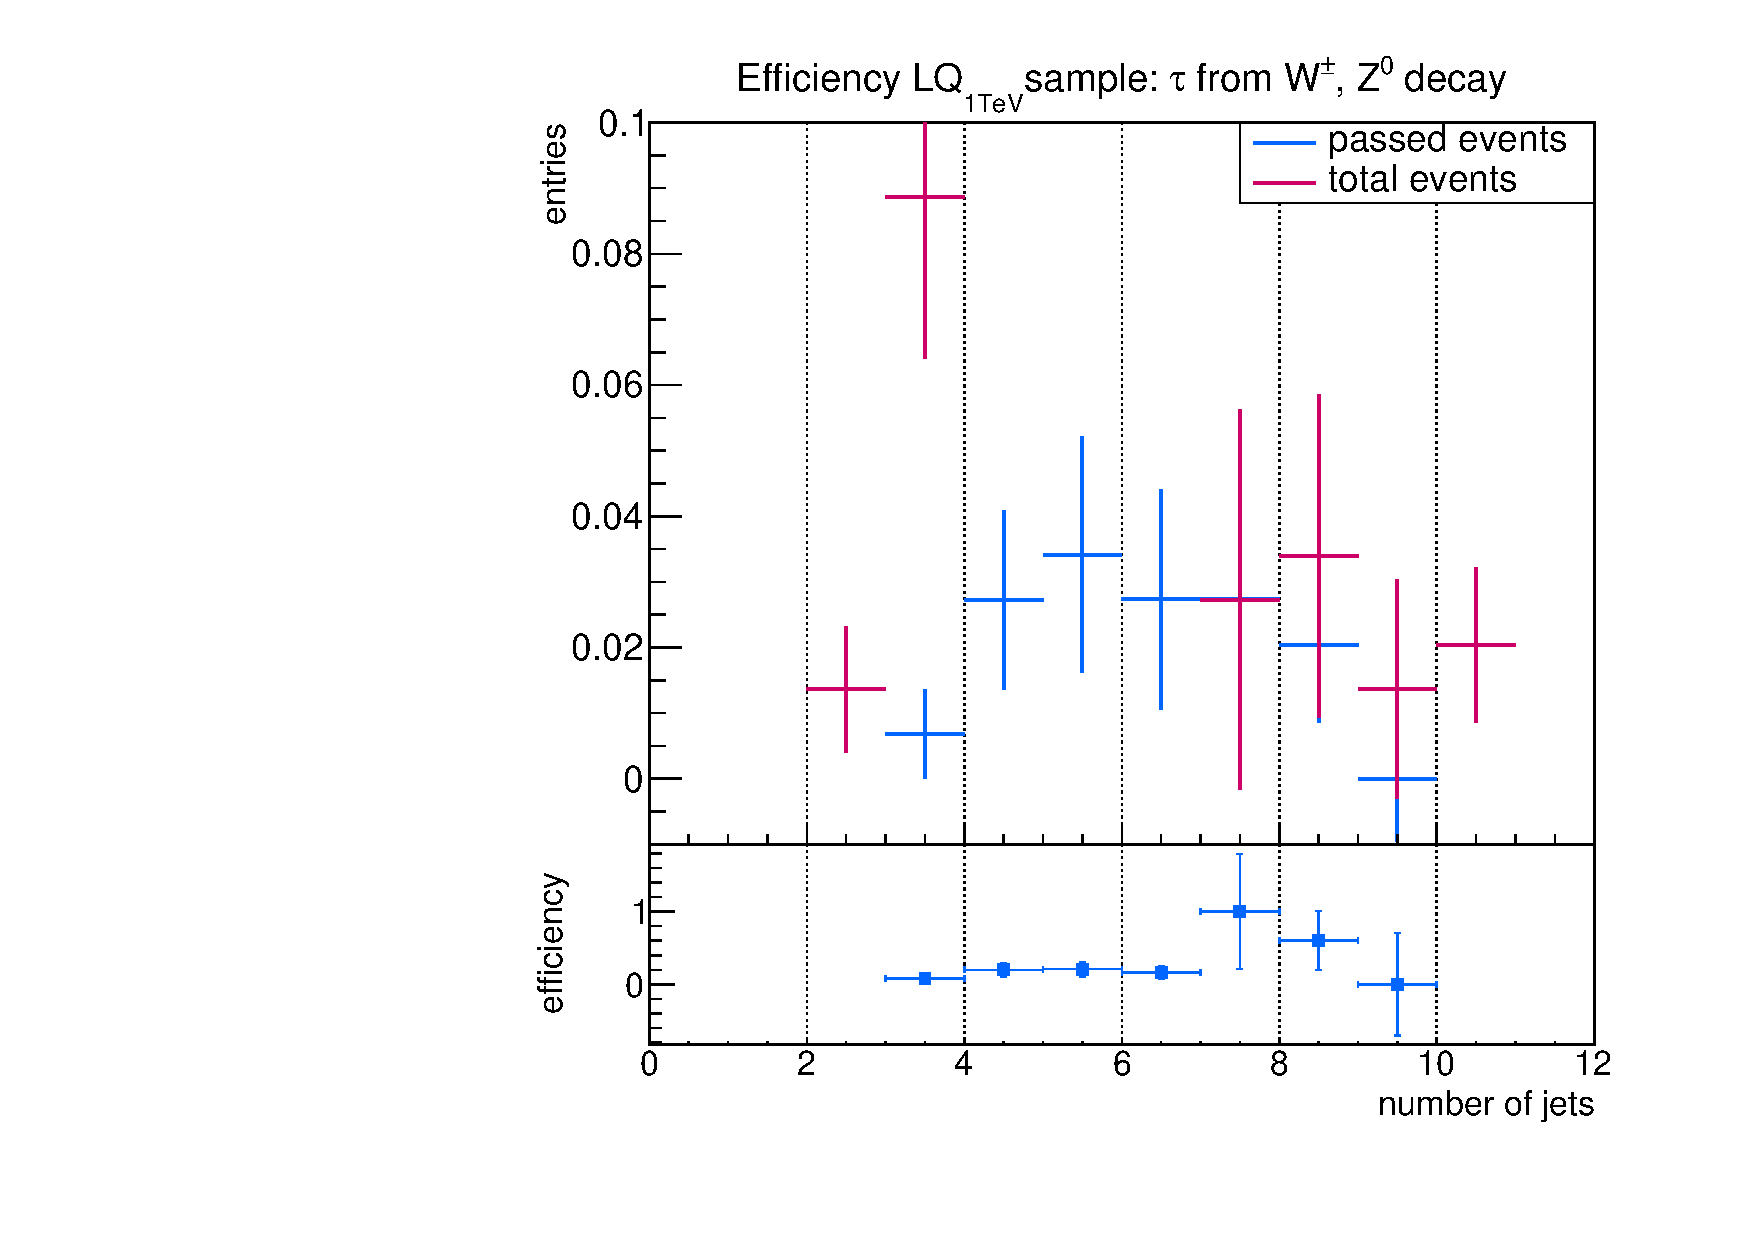
\includegraphics[width=\textwidth]{figures/plots/LQ76/Divided_promptnjets.pdf}
                \subcaption{Efficiency of taus originating from $W^\pm$, and $Z^0$ bosons depending on the number of jets for the LQ sample with high mass point.}
                \label{Dividedprompt:signal:njetsLQ76}
                \end{subfigure}
\caption[Efficiency of taus originating from LQs for the LQ signal events.]{Efficiency of taus originating LQs depending on the number of jets.}
\label{Divided:prompt:njets}
\end{figure}
%
%
\begin{figure}
  \centering
                \begin{subfigure}[t]{0.49\textwidth}
                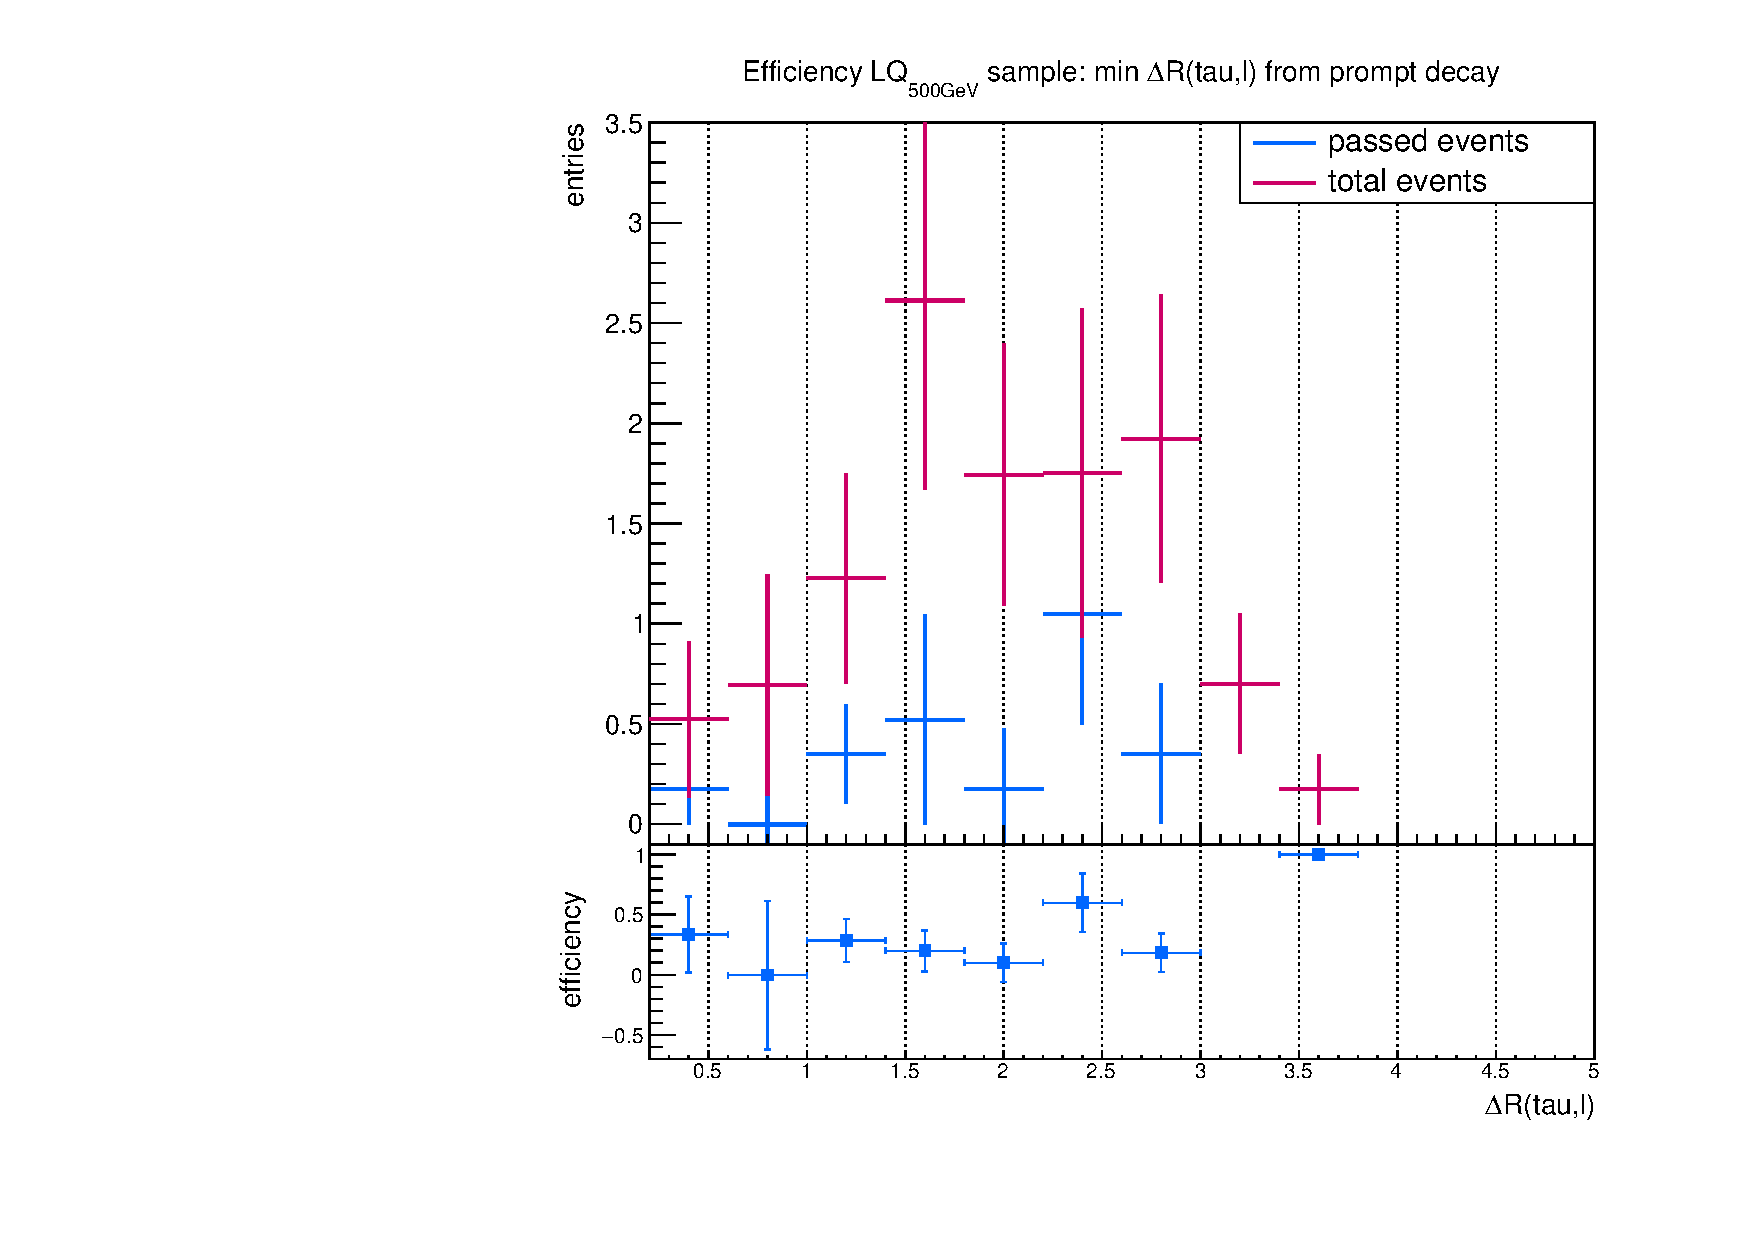
\includegraphics[width=\textwidth]{figures/plots/LQ75/Divided_pr_mindR_taulepton.pdf}
                \subcaption{Minimum separation between taus originating from $W^\pm$, $Z^0$ events and leptons for the low mass point LQ sample.}
                \label{dRprompt:signal:taulepton:minLQ75}
                \end{subfigure}
               %
                \begin{subfigure}[t]{0.49\textwidth}
                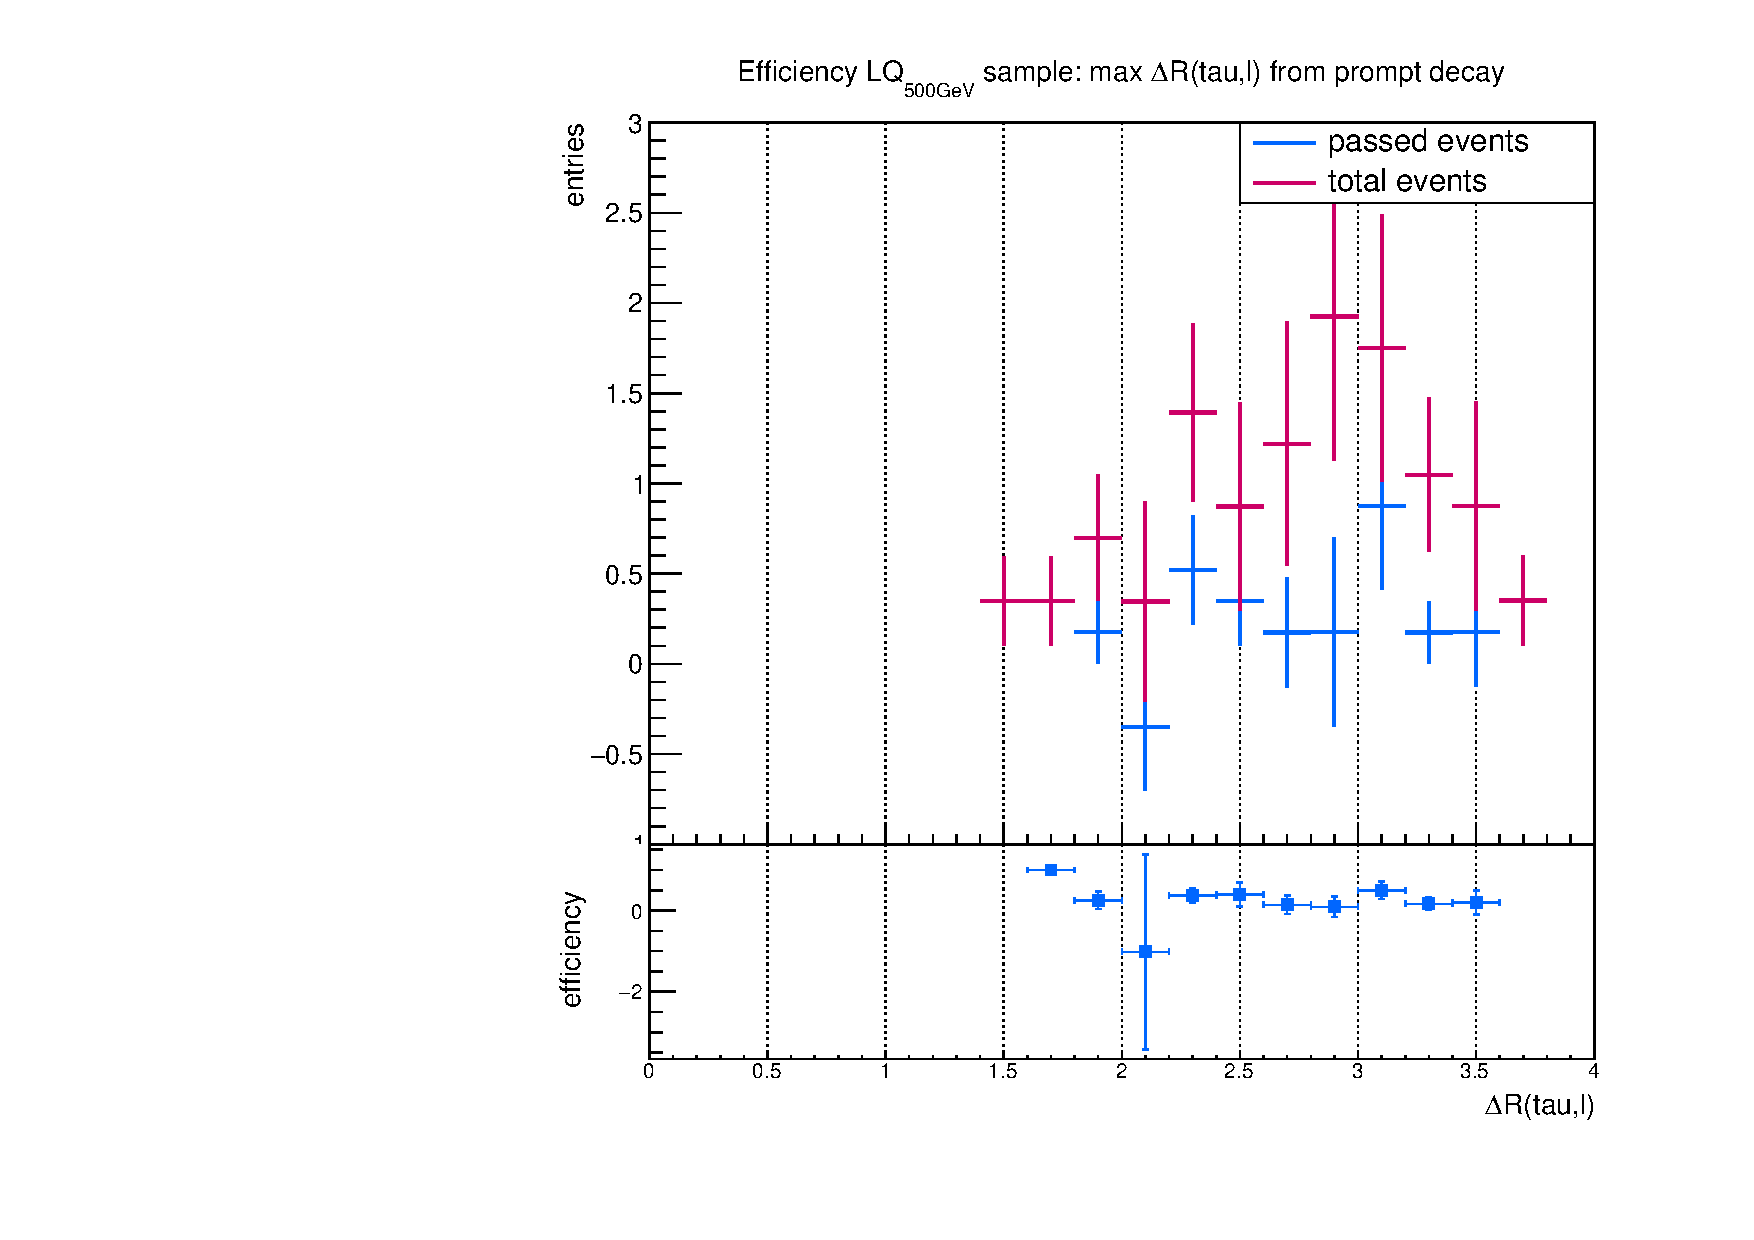
\includegraphics[width=\textwidth]{figures/plots/LQ75/Divided_maxdR_pr_taulepton.pdf}
                \subcaption{Maximum separation between taus originating from $W^\pm$, $Z^0$ events and leptons for the low mass point LQ sample.}
                \label{dRprompt:signal:taulepton:maxLQ75}
                \end{subfigure}
                 %
                \begin{subfigure}[t]{0.49\textwidth}
                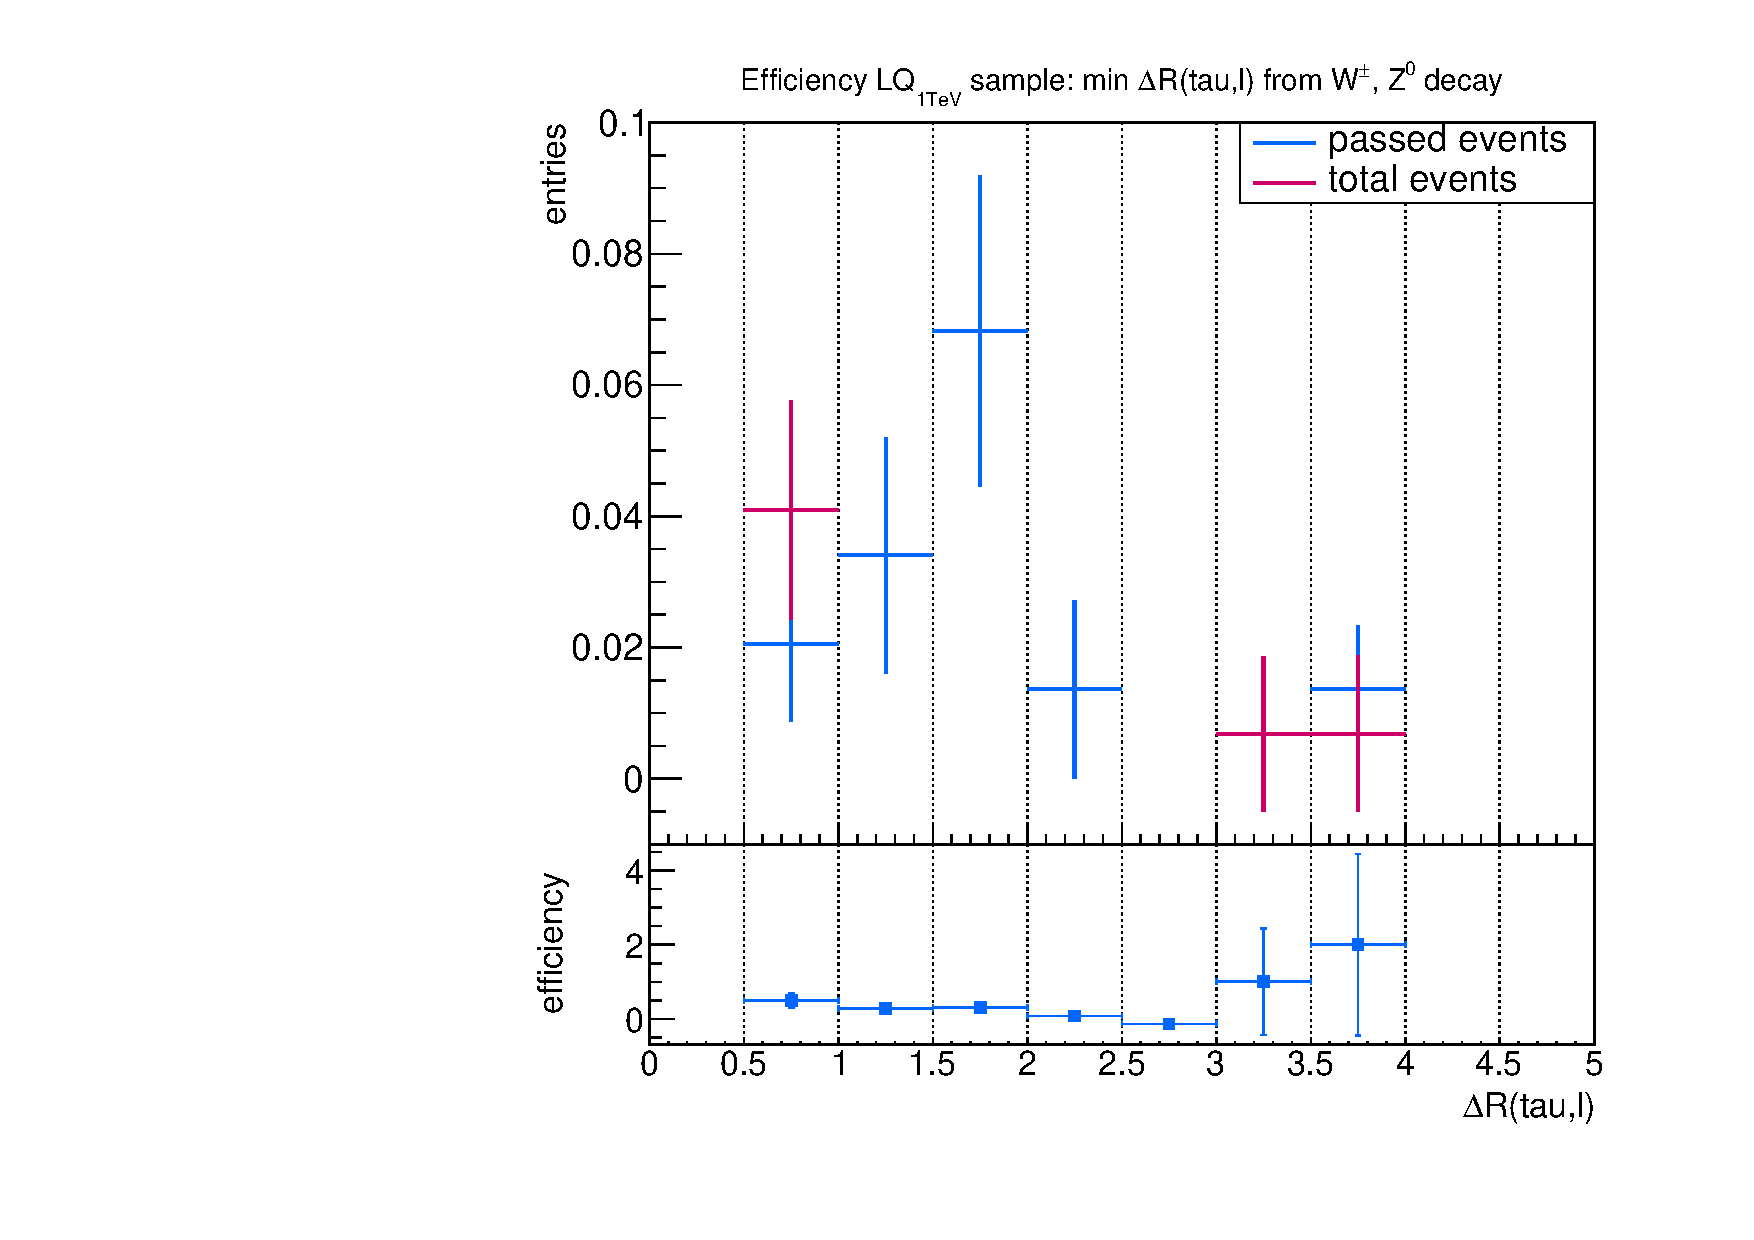
\includegraphics[width=\textwidth]{figures/plots/LQ76/Divided_pr_mindR_taulepton.pdf}
                \subcaption{Minimum separation between taus originating from $W^\pm$, $Z^0$ events and leptons for the high mass point LQ sample.}
                \label{dRprompt:signal:taulepton:minLQ76}
                \end{subfigure}
                 %
                \begin{subfigure}[t]{0.49\textwidth}
                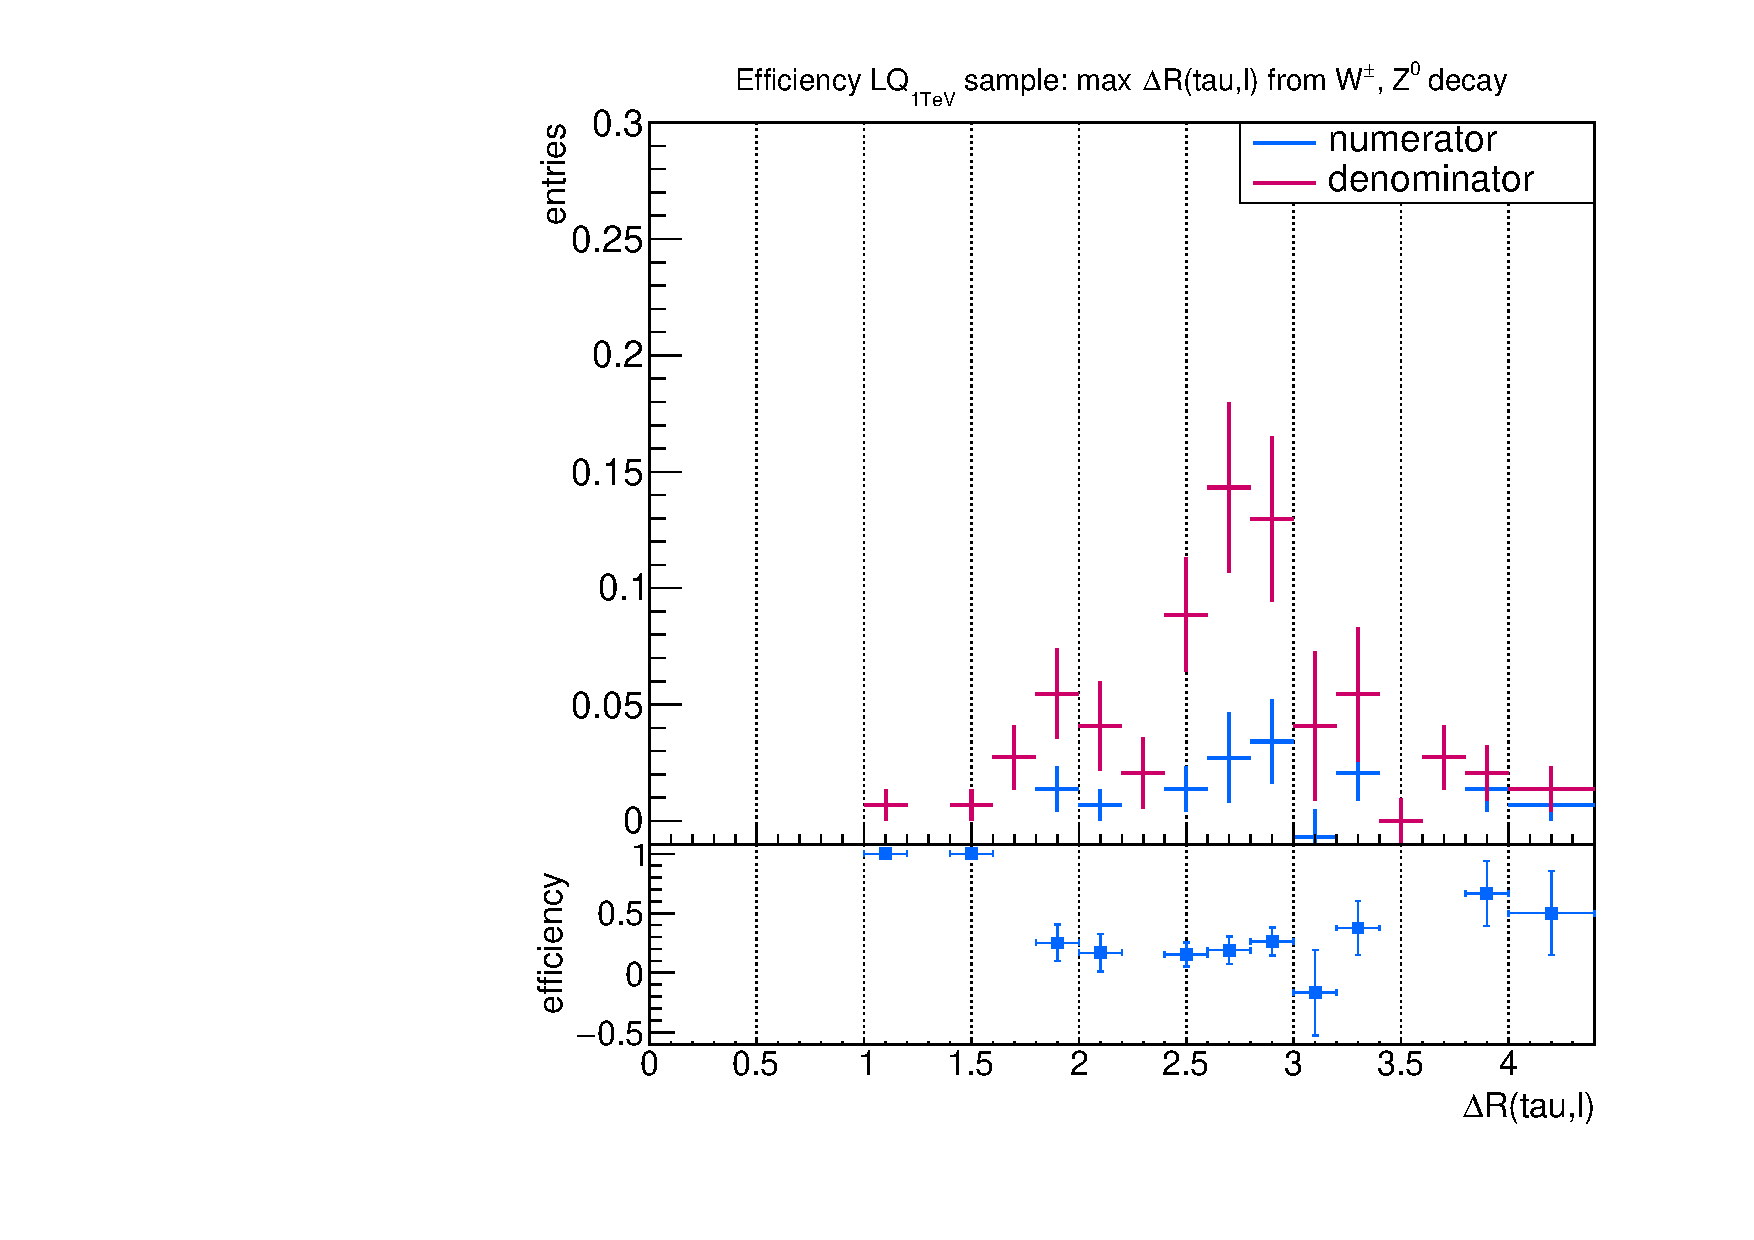
\includegraphics[width=\textwidth]{figures/plots/LQ76/Divided_maxdR_pr_taulepton.pdf}
                \subcaption{Maximum separation between taus originating from $W^\pm$, $Z^0$ events and leptons for the high mass point LQ sample.}
                \label{dRprompt:signal:taulepton:maxLQ76}
                \end{subfigure}
\caption[Efficiency of separation between taus originating from $W^\pm$, $Z^0$ and leptons.]{Efficiency of minimum and maximum separation between taus originating from $W^\pm$, $Z^0$ and leptons (electrons and muons).}
\label{dRprompt:signal:taulepton}
\end{figure}
%
%
\begin{figure}
  \centering
                \begin{subfigure}[t]{0.49\textwidth}
                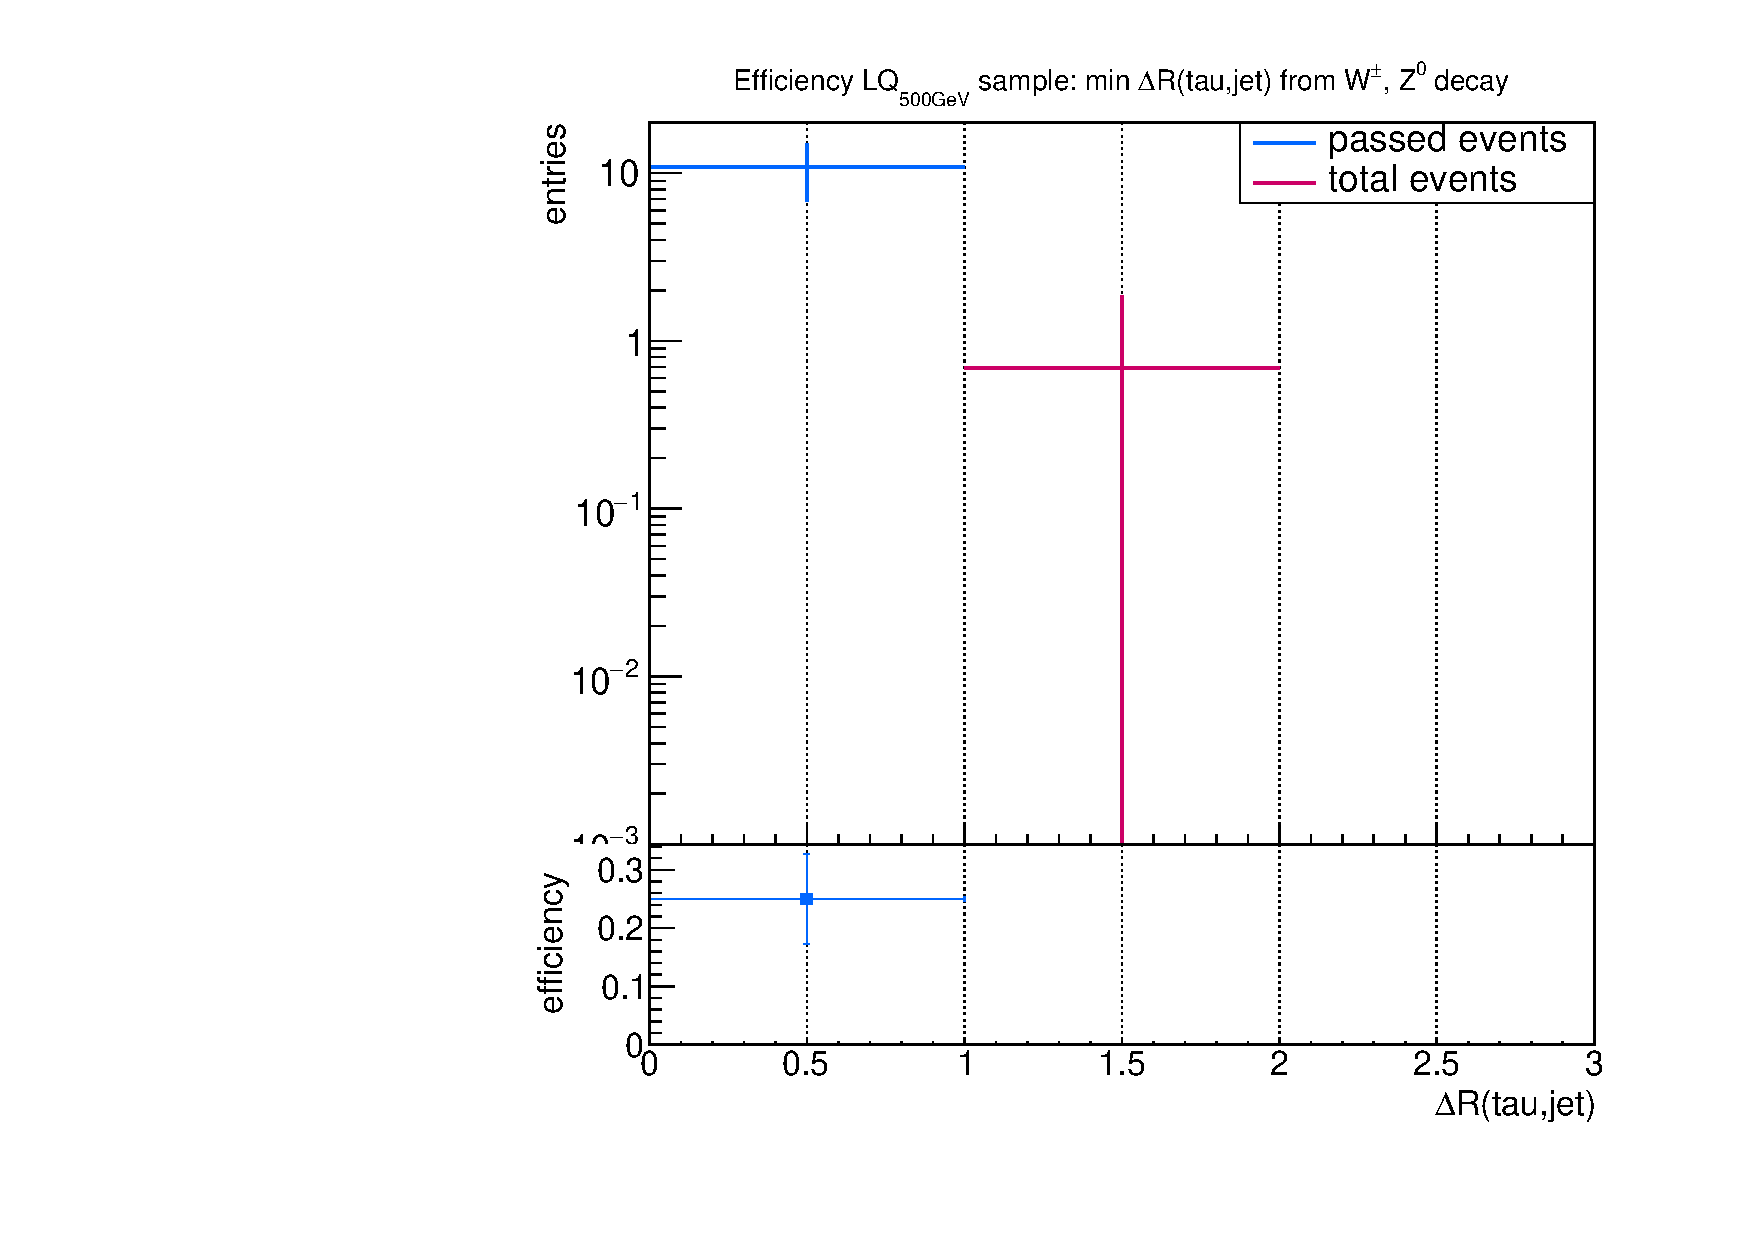
\includegraphics[width=\textwidth]{figures/plots/LQ75/Divided_pr_mindR_taujet.pdf}
                \subcaption{Minimum separation between taus originating from $W^\pm$, $Z^0$ events and jets for the low mass point LQ sample.}
                \label{dRprompt:signal:taujet:minLQ75}
                \end{subfigure}
                %
                \begin{subfigure}[t]{0.49\textwidth}
                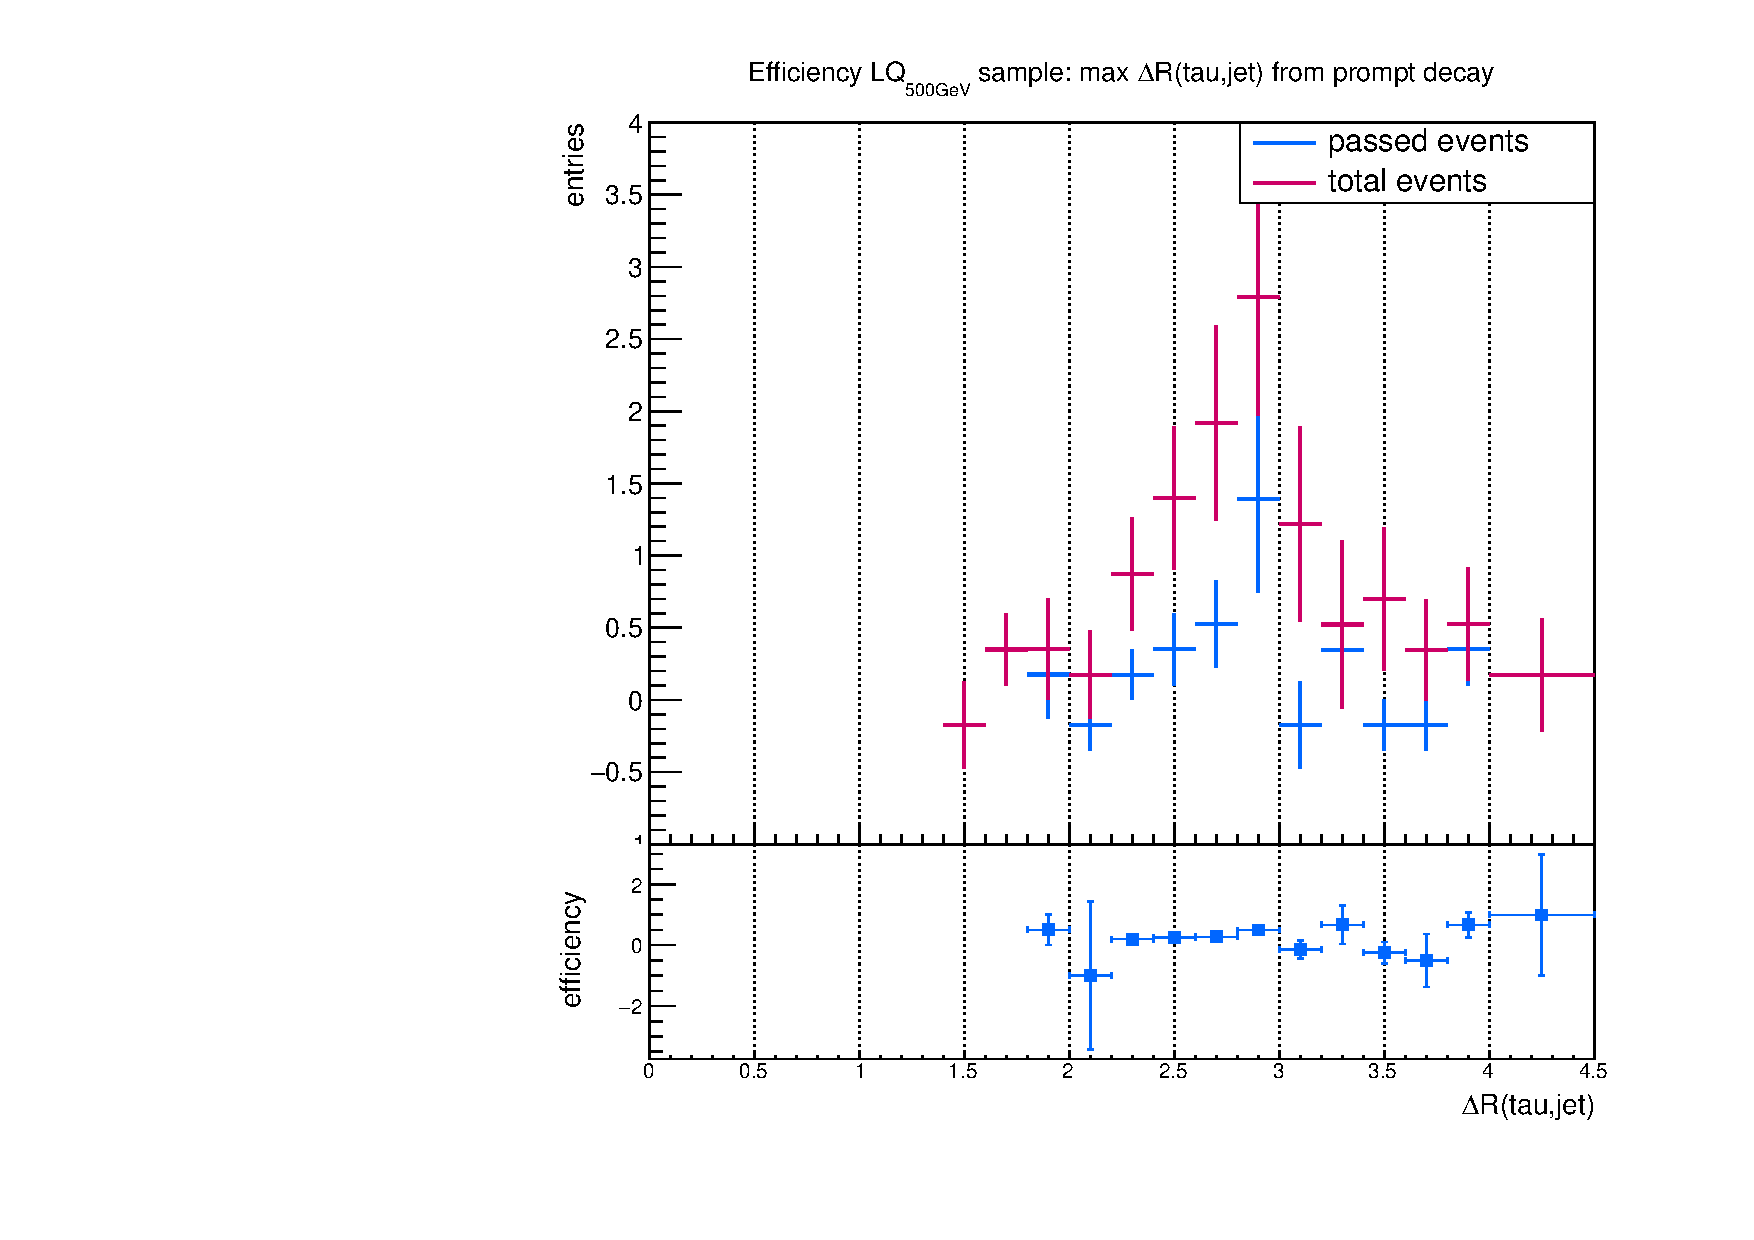
\includegraphics[width=\textwidth]{figures/plots/LQ75/Divided_maxdR_pr_taujet.pdf}
                \subcaption{Maximum separation between taus originating from $W^\pm$, $Z^0$ events and jets for the low mass point LQ sample.}
                \label{dRprompt:signal:taujet:maxLQ75}
                \end{subfigure}
                 %
                \begin{subfigure}[t]{0.49\textwidth}
                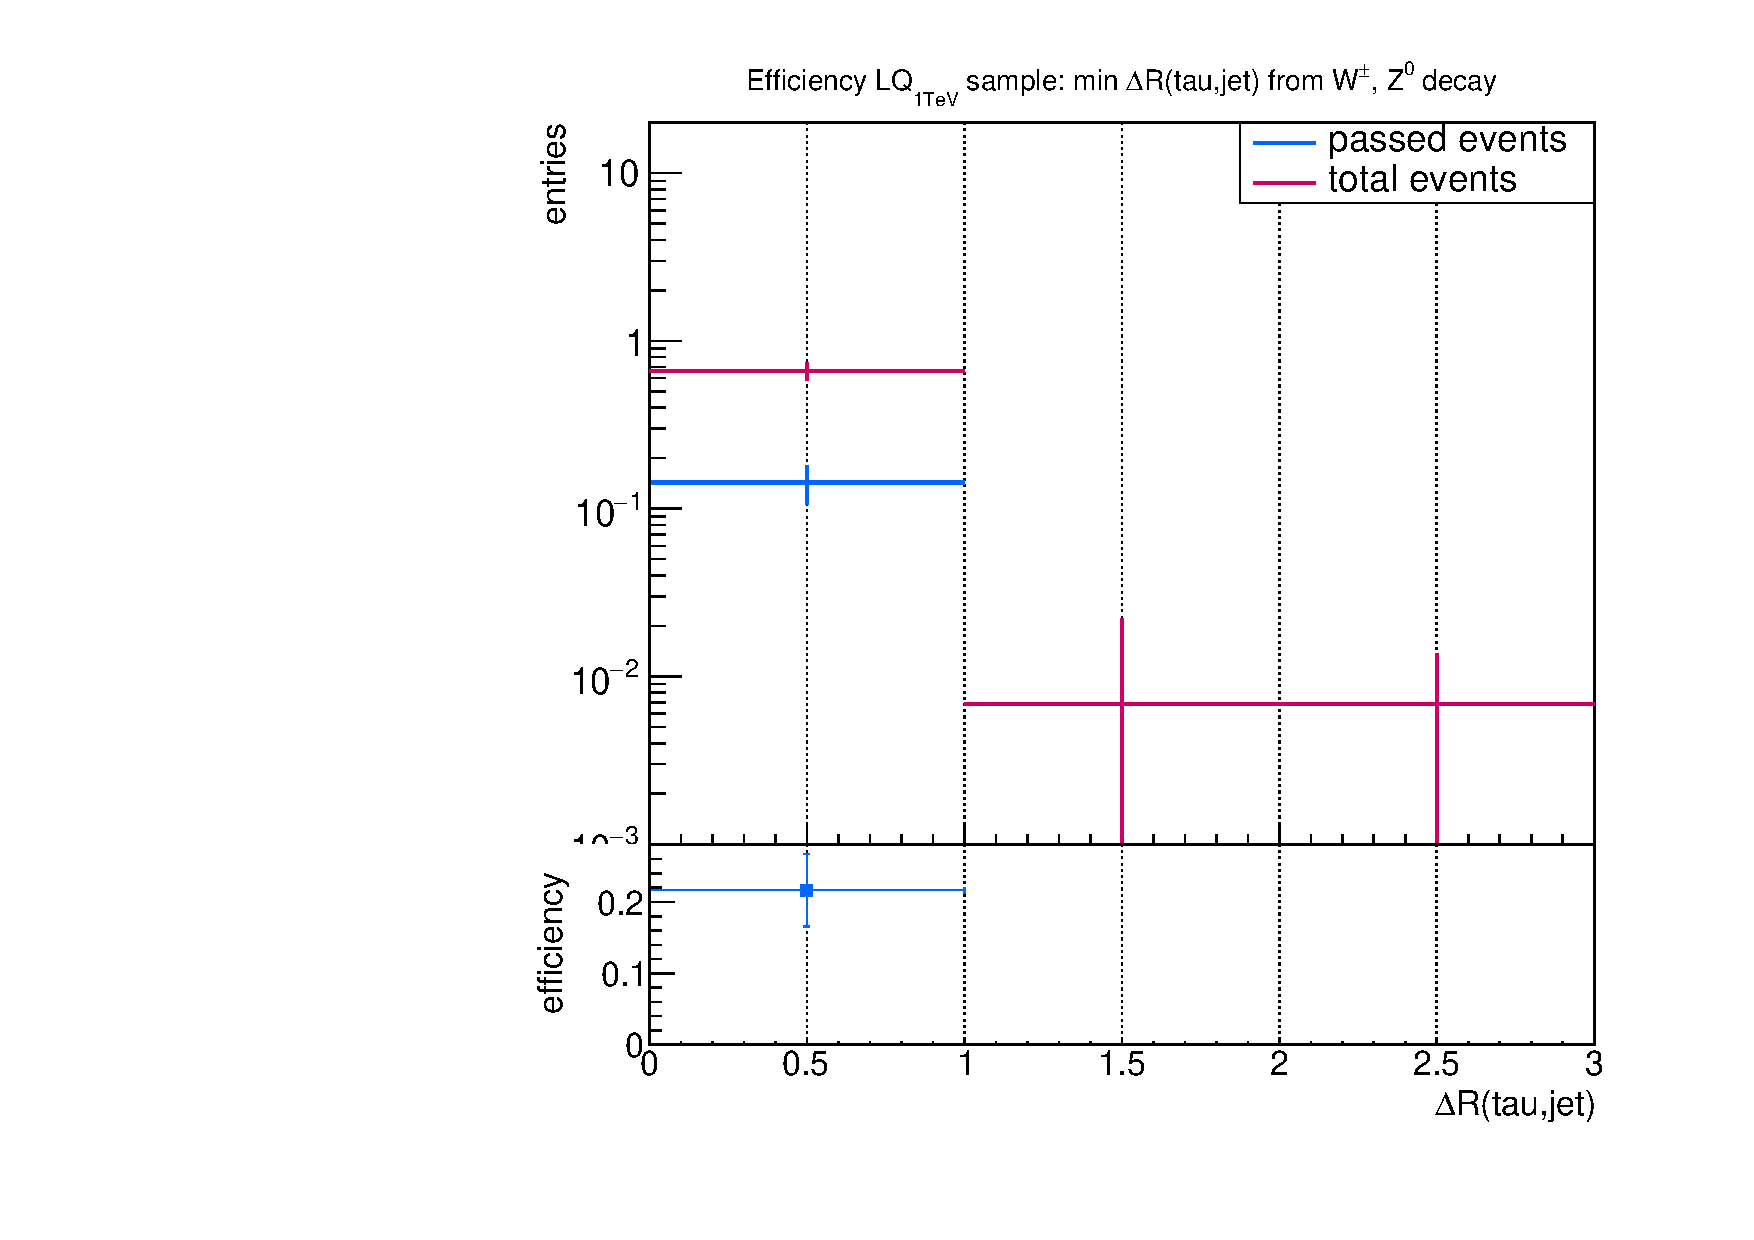
\includegraphics[width=\textwidth]{figures/plots/LQ76/Divided_pr_mindR_taujet.pdf}
                \subcaption{Minimum separation between taus originating from $W^\pm$, $Z^0$ events and jets for the high mass point LQ sample.}
                \label{dRprompt:signal:taujet:minLQ76}
                \end{subfigure}
                 %
                \begin{subfigure}[t]{0.49\textwidth}
                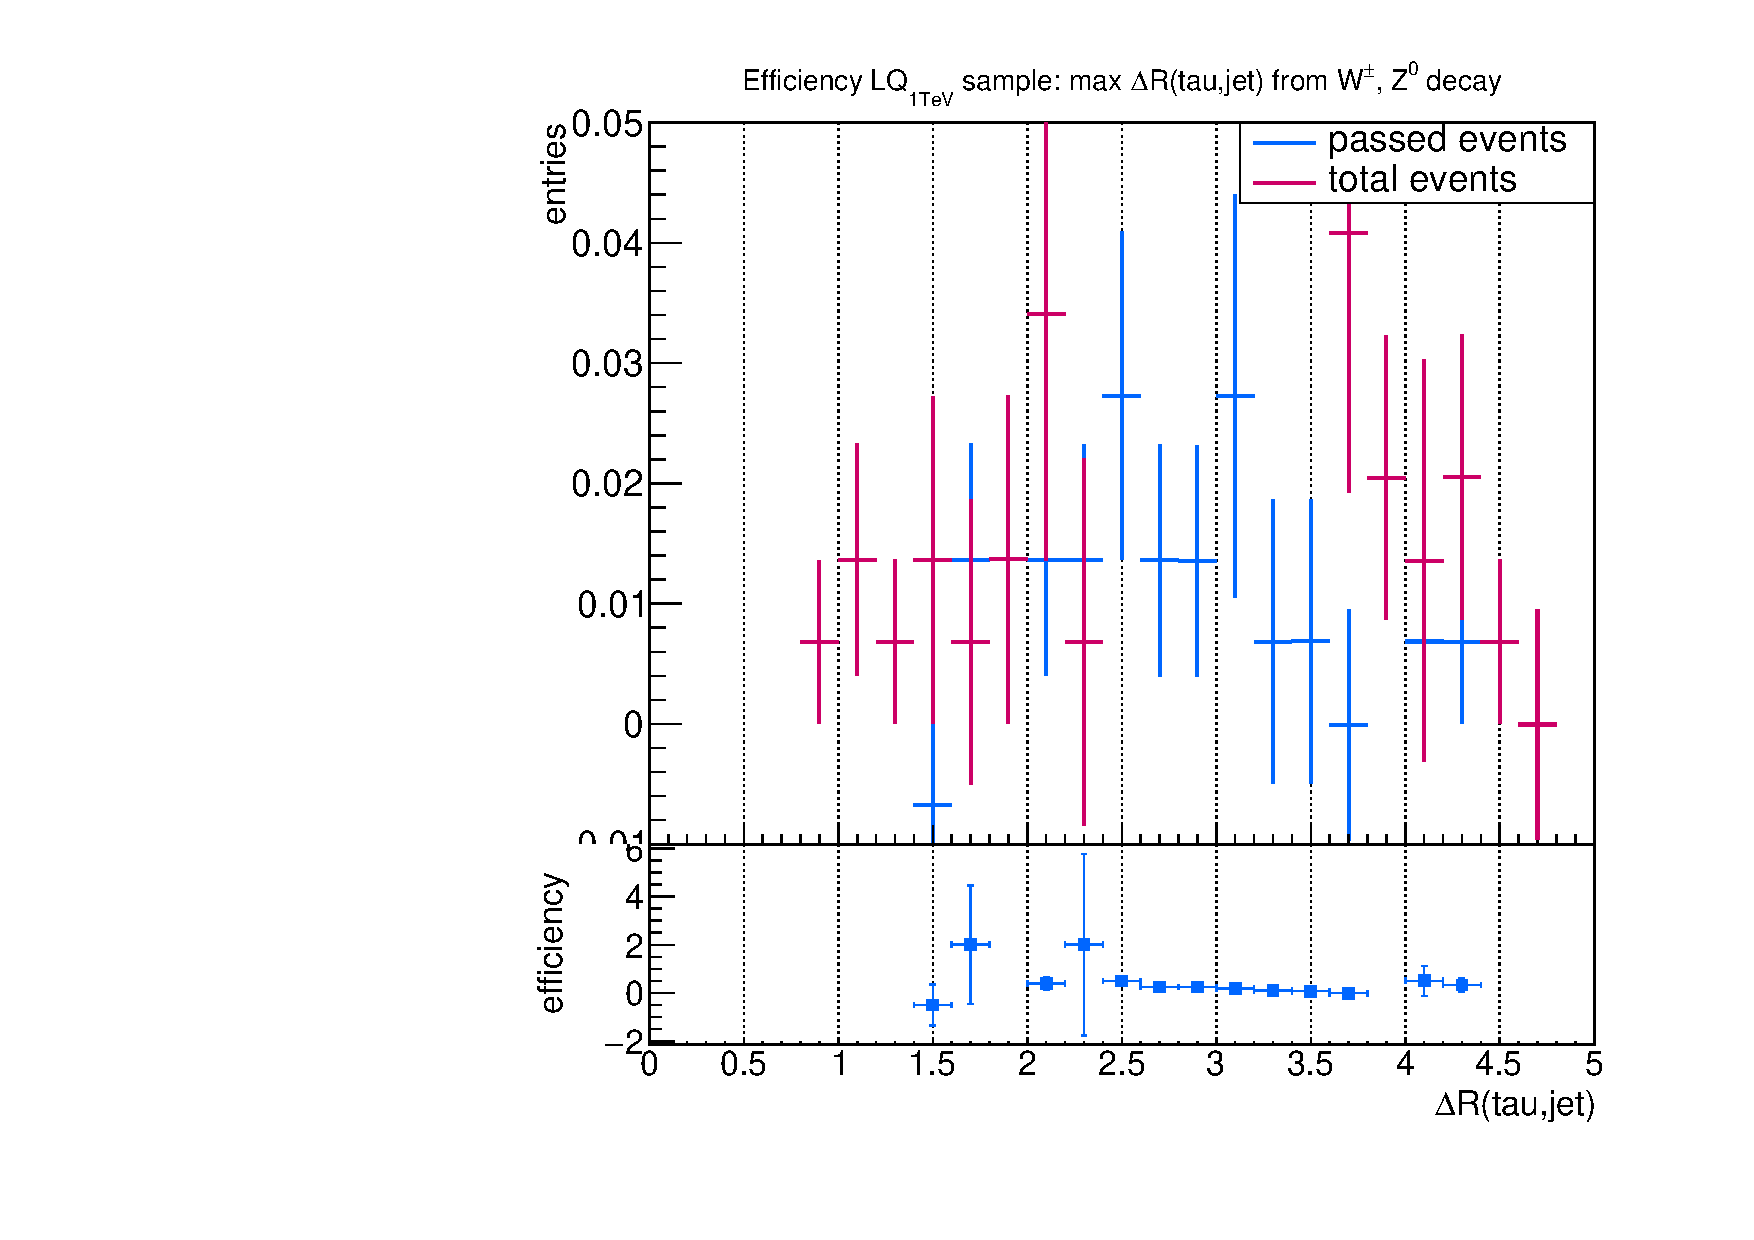
\includegraphics[width=\textwidth]{figures/plots/LQ76/Divided_maxdR_pr_taujet.pdf}
                \subcaption{Maximum separation between taus originating from $W^\pm$, $Z^0$ events and jets for the high mass point LQ sample.}
                \label{dRprompt:signal:taujet:maxLQ76}
                \end{subfigure}
\caption[Efficiency of separation between taus originating from $W^\pm$, $Z^0$ and jets.]{Efficiency of minimum and maximum separation between taus originating from $W^\pm$, $Z^0$ and jets.}
\label{dRprompt:signal:taujet}
\end{figure}
%
%
\begin{figure}
  \centering
                \begin{subfigure}[t]{0.49\textwidth}
                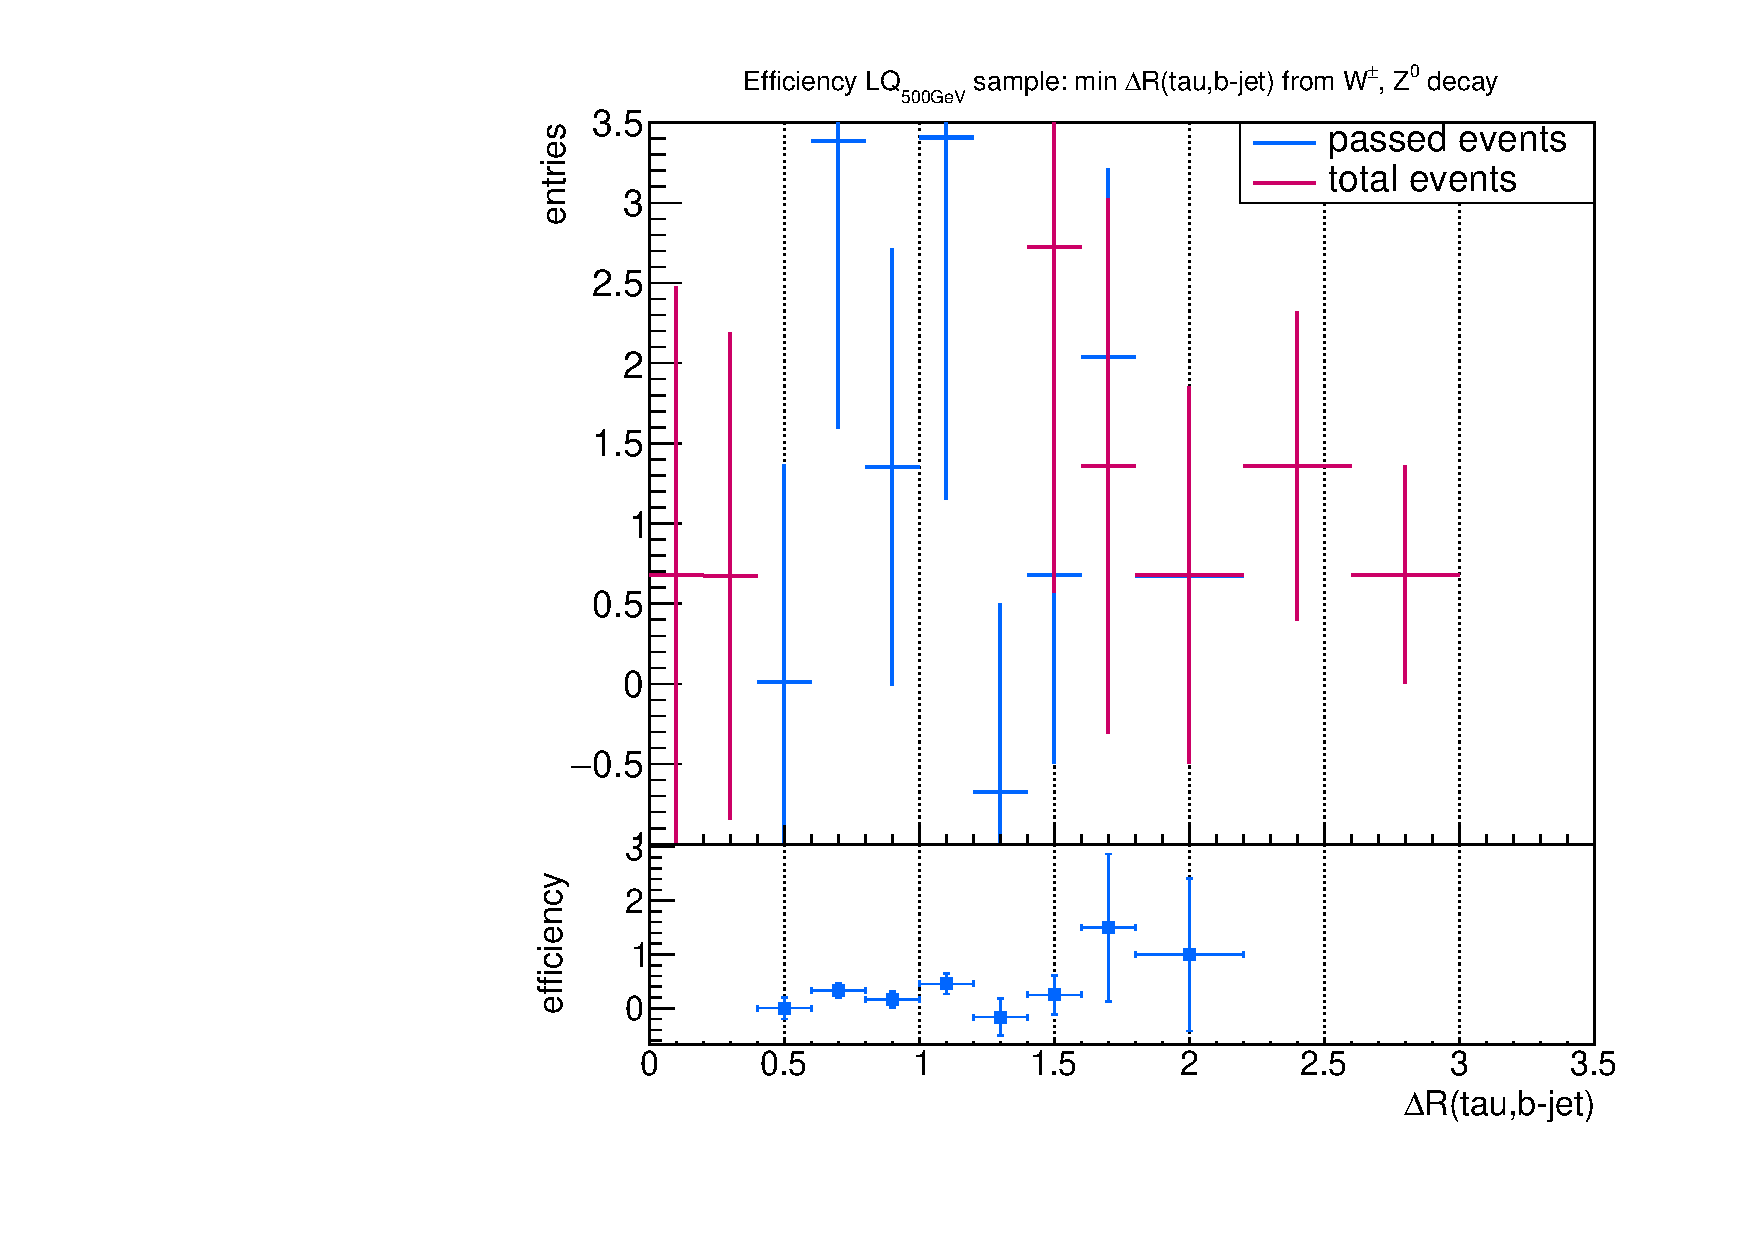
\includegraphics[width=\textwidth]{figures/plots/LQ75/Divided_mindR_pr_taubjet.pdf}
                \subcaption{Minimum separation between taus originating from $W^\pm$, $Z^0$ events and b-jets for the low mass point LQ sample.}
                \label{dRprompt:signal:taubjet:minLQ75}
                \end{subfigure}
                %
                \begin{subfigure}[t]{0.49\textwidth}
                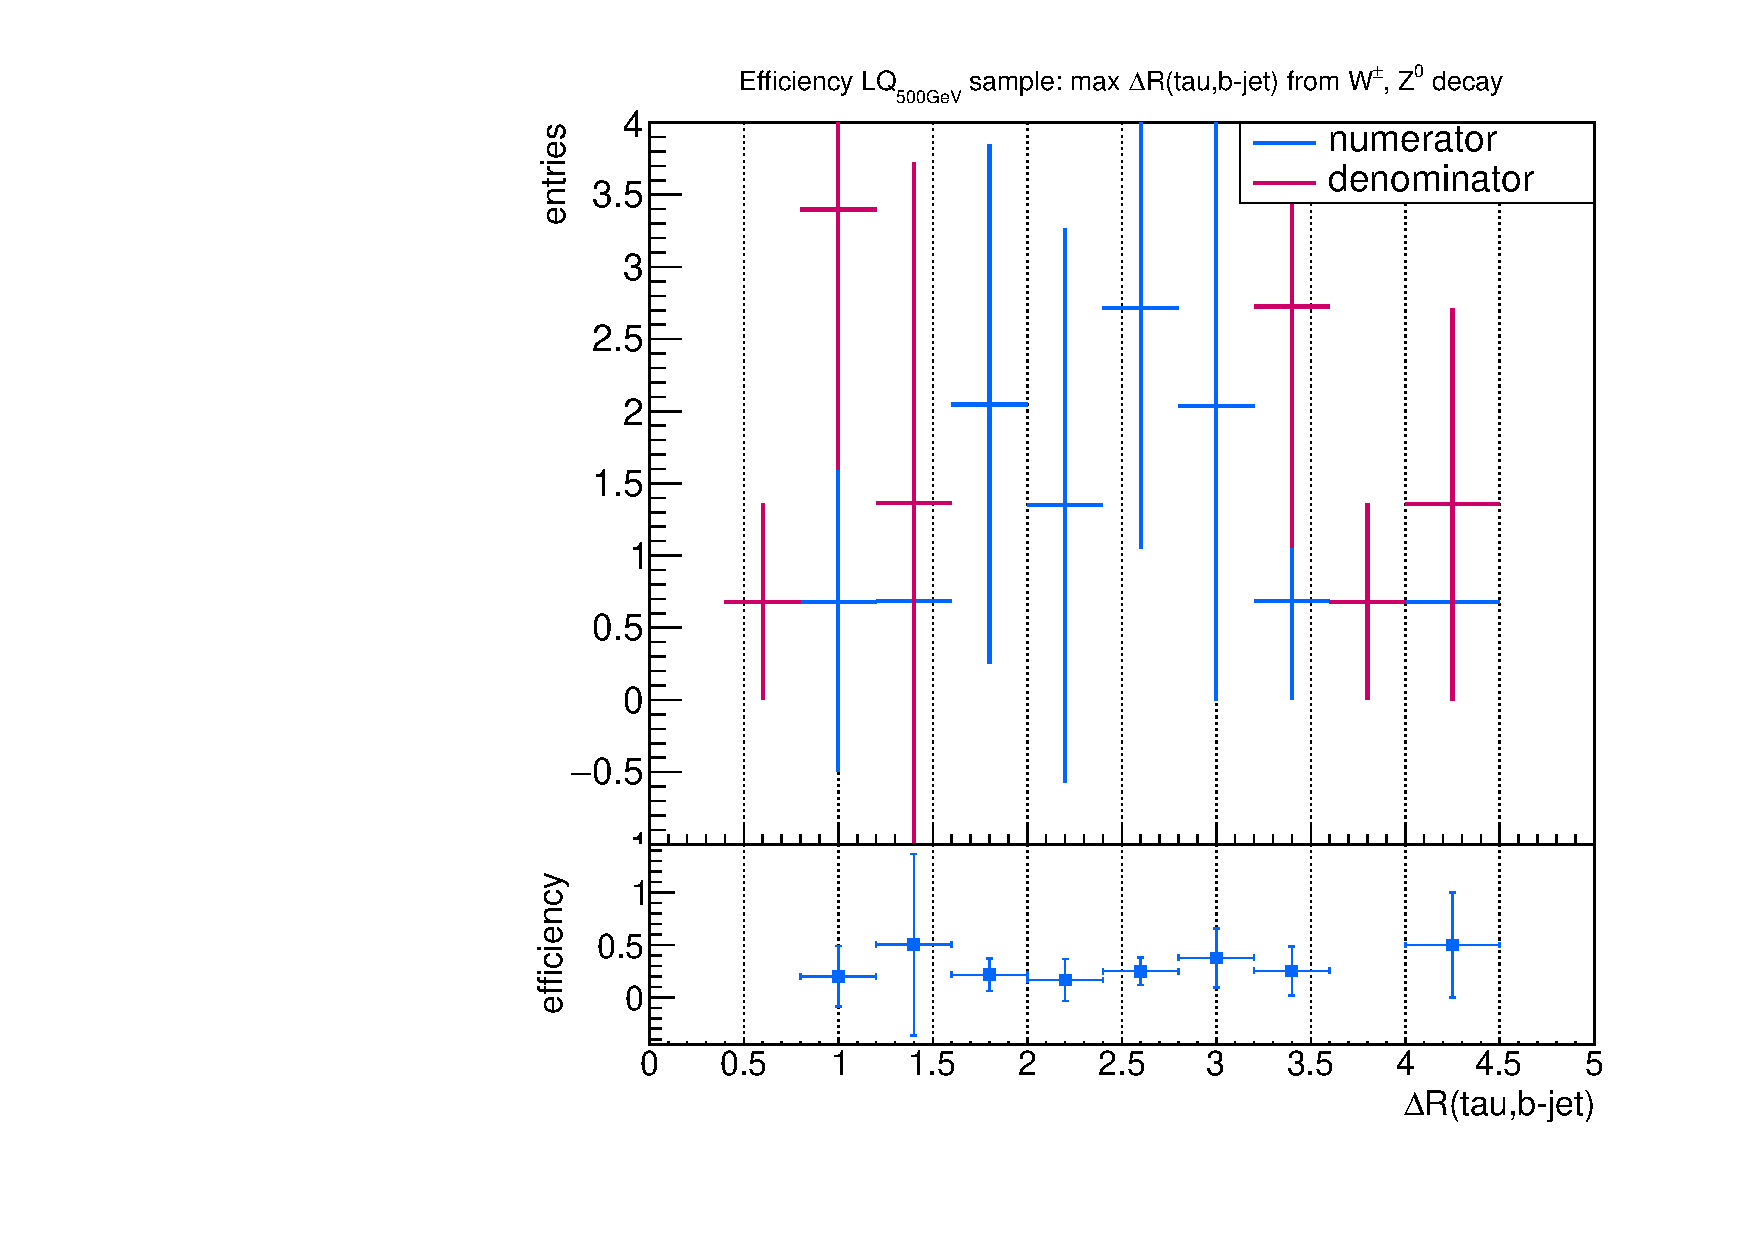
\includegraphics[width=\textwidth]{figures/plots/LQ75/Divided_maxdR_pr_taubjet.pdf}
                \subcaption{Maximum separation between taus originating from $W^\pm$, $Z^0$ events and b-jets for the low mass point LQ sample.}
                \label{dRprompt:signal:taubjet:maxLQ75}
                \end{subfigure}
                 %
                \begin{subfigure}[t]{0.49\textwidth}
                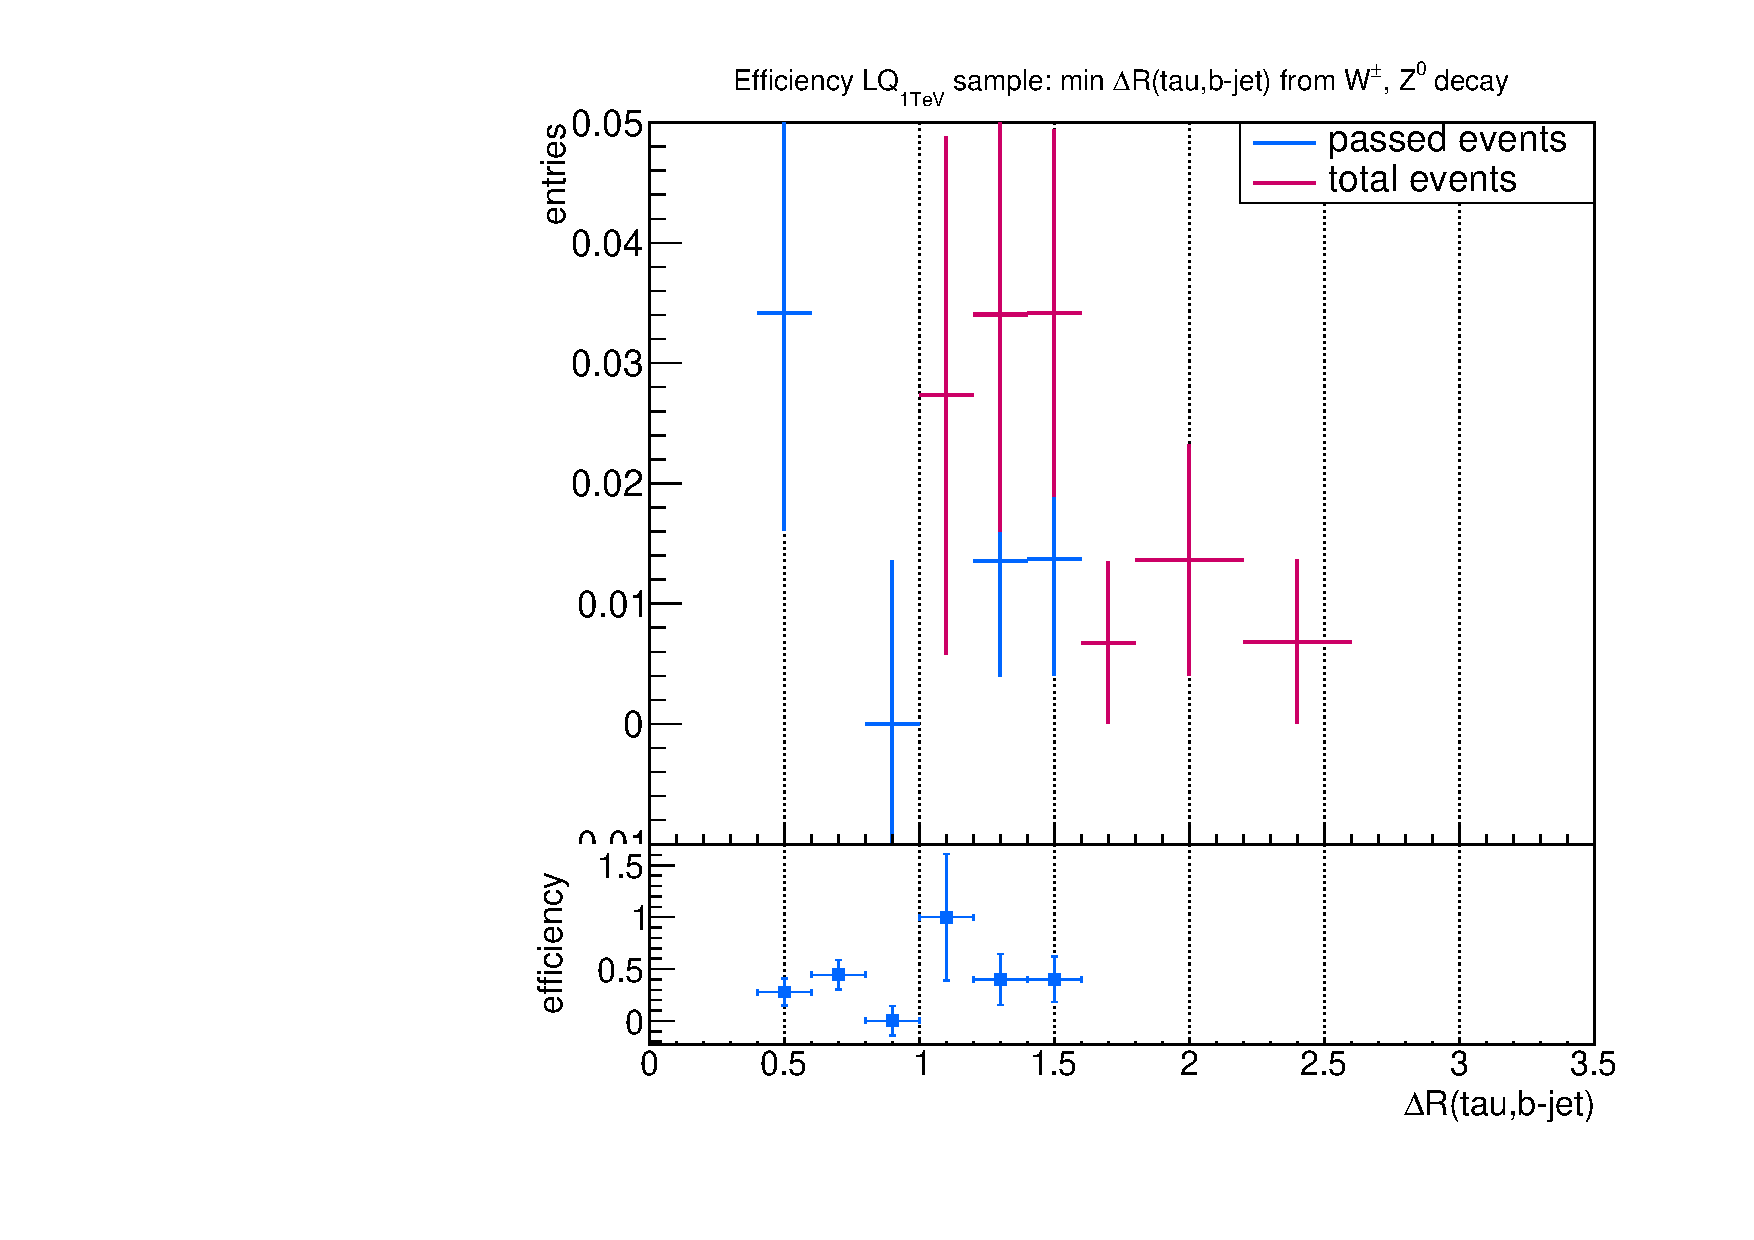
\includegraphics[width=\textwidth]{figures/plots/LQ76/Divided_mindR_pr_taubjet.pdf}
                \subcaption{Minimum separation between taus originating from $W^\pm$, $Z^0$ events and b-jets for the high mass point LQ sample.}
                \label{dRprompt:signal:taubjet:minLQ76}
                \end{subfigure}
                 %
                \begin{subfigure}[t]{0.49\textwidth}
                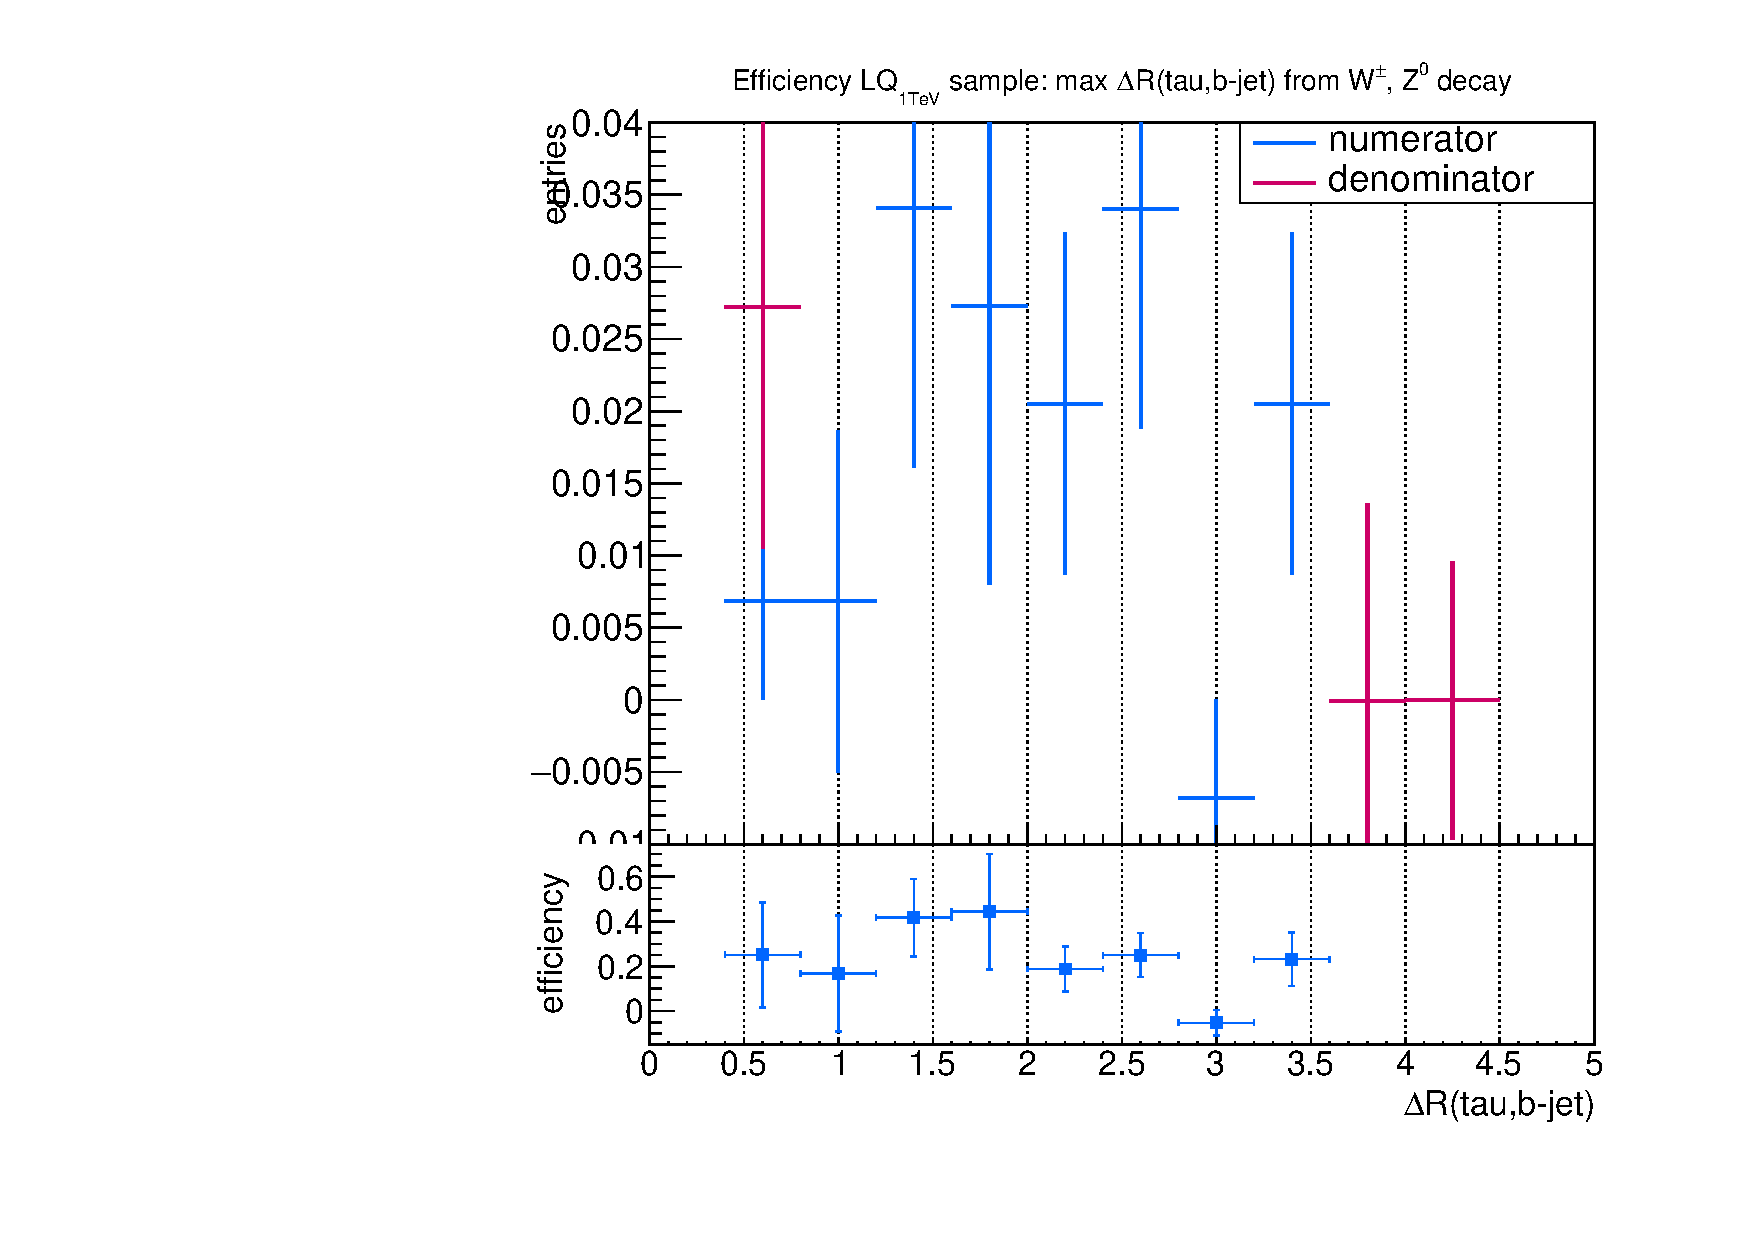
\includegraphics[width=\textwidth]{figures/plots/LQ76/Divided_maxdR_pr_taubjet.pdf}
                \subcaption{Maximum separation between taus originating from $W^\pm$, $Z^0$ events and b-jets for the high mass point LQ sample.}
                \label{dRprompt:signal:taubjet:maxLQ76}
                \end{subfigure}
\caption[Efficiency of separation between taus originating from $W^\pm$, $Z^0$ and b-jets.]{Efficiency of minimum and maximum separation between taus originating from $W^\pm$, $Z^0$ and b-jets.}
\label{dRprompt:signal:taubjet}
\end{figure}

